\documentclass[11pt,fleqn,oneside]{book}

\usepackage[english]{babel}
\usepackage[latin1]{inputenc}
\usepackage{amsmath,amsfonts,amssymb,makeidx,epsfig}
\usepackage{longtable,multicol}
\usepackage[english]{varioref}
\usepackage[gen,right]{eurosym}
\usepackage{dsfont}
\usepackage{natbib}
\usepackage{graphics}
\usepackage{color}
\usepackage{newlfont}
\usepackage{lscape}
\usepackage{subfigure}
\usepackage{pstricks,pstricks-add,pst-plot}
\usepackage{dsfont}
\usepackage{url}

\newtheorem{theorem}{Theorem}[section]
\newtheorem{proposition}{Proposition}[section]
\newtheorem{definition}{Definition}[section]
\newtheorem{corollary}{Corollary}[section]
\newtheorem{lemma}{Lemma}[section]
\newtheorem{assumption}{Assumption}[section]
\newtheorem{tempass}{Temporary Assumption}[section]
\newtheorem{remark}{Remark}[section]
\newtheorem{homework}{Homework}
\newtheorem{observation}{Observation}
\newtheorem{exercise}{Exercise}

\setlength{\oddsidemargin}{.1in}     % set left margin 1.6 inch
\setlength{\evensidemargin}{.1in}    % set right margin 1.1 inch
\setlength{\textwidth}{6.4in}        % set text width = 6 inch
\setlength{\textheight}{8.2in}       % set text length = 8.2 inch

%\def\blfootnote{\xdef\@thefnmark{}\@footnotetext}

\begin{document}
\begin{titlepage}
\newlength{\widthOne} \newlength{\widthTwo}
\centering\Large\sffamily
\settowidth{\widthOne}{\fontsize{35}{50}\selectfont U Wisconsin}
\settowidth{\widthTwo}{\fontsize{17}{20}\selectfont\bfseries
Class notes ActSci 650}
\vspace*{\fill}


\includegraphics[height=2.3cm]{Graphs/wisc.png}
%\parbox[b]{\widthOne}{
%\fontsize{35}{50}\selectfont Georgia State\\ University 
 %}
\quad\rule[-12pt]{1mm}{90pt}\quad
\parbox[b]{\widthTwo}{\fontsize{17}{20}\selectfont\bfseries 
 Class notes \\ActSci 650\\ Actuarial Maths I}\\
%Last Revised on \revised\\

\vfill			

Dr.\ Daniel Bauer 		\\%[18pt]
Department of Risk and Insurance				\\
Wisconsin School of Business					\\ 
University of Wisconsin-Madison				\\
975 University Avenue, Madison, WI 53706				\\
daniel.bauer@wisc.edu\\

\vspace{2.5cm}
{\footnotesize
Based on \cite{BOWERS} as well as the lecture notes by R\"{u}diger Kiesel (Ulm University), Ragnar Norberg (London School of Economics), Eric Ulm (Georgia State University), Shaun Wang (Georgia State University), and Hans-Joachim Zwiesler (Ulm University).
}

\vfill
{\large \textbf{Fall 2019}}
\end{titlepage}


\setcounter{secnumdepth}{3} % bis subsubsection wird nummeriert
\renewcommand{\thesubsubsection}{\alph{subsubsection})} % diese dann allerdings mit a), b)
\setcounter{tocdepth}{2}    % aber nur Eintr"age bis x.y.z (subsection) in Inhaltsverzeichnis
\addcontentsline{toc}{chapter}{\contentsname} %
\tableofcontents %
\cleardoublepage %

% Abbildungsverzeichnis
%\addcontentsline{toc}{chapter}{\listfigurename} %
%\listoffigures %
%\cleardoublepage %

% Tabellenverzeichnis
%\addcontentsline{toc}{chapter}{\listtablename} %
%\listoftables %
%\cleardoublepage %

% Abk"urzungsverzeichnis
%\include{dat/!Abk} %
%\cleardoublepage %

\mainmatter     % Hauptteil der Arbeit

\renewcommand*{\thechapter}{\arabic{chapter}} %
\renewcommand*{\thesection}{\thechapter.\arabic{section}} %

\chapter{Syllabus}

\section*{Class Information}
\begin{itemize}
\item \textbf{Credits}: 3
%\item \textbf{Course Designations:} General Business 
\item \textbf{Location:} 3070 Grainger Hall
\item \textbf{Time/Dates:}  TR 11:00 am - 12:15 pm
\item  \textbf{Canvas Course URL:}  \url{https://canvas.wisc.edu/courses/153634}
\item \textbf{Instructional Mode}: All face-to-face 
 \item  \textbf{Prerequisites:} MATH 303 and (STAT/MATH  309, STAT 311, or STAT/MATH  431); or member of Business Exchange program.  Basic familiarity with Microsoft Excel and \textbf{R} (\url{http://www.r-project.org}) is assumed.  
 \item \textbf{How this Course Meets the Credit Hour Policy Standard:} This class meets for two 75-minute class periods each week over the fall/spring semester and carries the expectation that students will work on course learning activities (reading, writing, problem sets, studying, etc.) for about 3 hours out of classroom for every class period. The syllabus includes more information about meeting times and expectations for student work. 
\end{itemize}

\subsection*{Catalog Description}

Advanced problems in the mathematical theory of life contingencies; force of mortality, laws of mortality; premiums and reserves for insurance and annuities based on a single life. 

\section*{Instructor Information}
\begin{itemize}
\item \textbf{Instructor:} Daniel Bauer, Associate Professor of Risk \& Insurance and Hickman-Larson Chair in Actuarial Science
\item \textbf{Office:} 5251 Grainger Hall
\item \textbf{Office Hours:} T 12:30pm-1:15pm, R 1:00pm-1:45pm
\item \textbf{Phone:} (608) 265-4119
\item \textbf{Email:} Daniel.Bauer@wisc.edu
\end{itemize}

\subsection*{Textbooks}

\section*{Course Learning Outcomes}

\begin{enumerate}
\item Develop survival models and life tables. 
\item Utilize survival models and life tables to calculate quantities pertaining to the future lifetime of a single life.
\item Calculate non-parametric estimates of survival models and describe and apply simple longevity models.
\item Determine quantities derived from the present value (of the future benefit) distribution of traditional life insurances, including whole life, term life, and endowment insurance.
\item Determine quantities derived from the present value (of the future payments) distribution of traditional life annuities, including whole life, term/temporary life, and guaranteed/certain and life annuities.
\item Calculate premium payments (level and non-level) for traditional life insurances and life annuities.
\end{enumerate}


\section*{Methods of Instruction}

The material will be presented in lecture form.  As a general approach, I first discuss models and methods conceptually, and I then provide and discuss a variety of example problems/programs that illustrate the concepts.  Depending on the subject, the theoretical and practical illustration may be in sequence or in parallel.

\subsection*{Attendance Policy}

Attendance is not formally taken. However, it is strongly suggested that students do not miss class as most students will have difficulties completing the assignments without attending the lectures.

\subsection*{Exam Structure and Grading Criteria}

There will be tentatively 8 weekly quizzes (18 minutes each Thursday unless noted otherwise - see tentative outline below), one mid-term examination, and one final examination.  The final exam covers the entire course with emphasis on the more recent material. Students who miss examinations should contact me immediately. Make-up examinations are only offered under extraordinary circumstances (e.g.\ sickness attested by a medical certificate or affirmation by the Dean of Students office). The lowest quiz score (missed quizzes receive a '0' score) will be dropped/disregarded. Please contact me if you miss more than one quiz; under extraordinary circumstances, special arrangements can be made.

Weekly homework will be assigned and collected irregularly. Moreover, there will be a few Excel and R assignments that should be submitted via Canvas. Late work will not be accepted.    

The grading of students' performance in this course is based on the following breakdown:
\begin{center}
\begin{tabular}{|l | l |}
\hline
Homework		& 5\%  \\
Quizzes	  		& 30\% \\
Mid-Term Exam	& 30\% \\
Final Exam 		& 35\% \\ 
\hline
\end{tabular}
\end{center}

The following grade scale applies:
\begin{center}
\begin{tabular}{ | c | c | c | c | c | c | c |}
\hline
 \textbf{ A } & \textbf{ AB} & \textbf{ B} & \textbf{ BC} & \textbf{ C} & \textbf{ D } & \textbf{ F } \\    
\hline
 93 & 89 & 80 & 75 & 65 & 55 & $<55$ \\
\hline  
\end{tabular}
\end{center}

Class attendance and participation is not graded.

Final grades may be curved slightly at the discretion of the instructor. In the event any curve is applied, the grading scale will not be adjusted to make the attainment of a letter grade more difficult.

\subsection*{Attendance Policy}
It is strongly suggested that students do not miss classes as, historically, students with multiple absences perform poorly on quizzes/examinations and have extreme difficulty in completing the course successfully. However, grades will not be subject to students' attendance or participation.

\subsection*{Suggested Textbook}

\textit{Actuarial Mathematics for Life Contingent Risks}, Second Edition, 2013, by Dickson, C.M.D., Hardy, M.R., and Waters, H.R. Cambridge: Cambridge University Press. Chapters 1-7.5.

Additionally, lecture notes and the relevant study notes will be posted on Canvas. Note that it is strongly advised that you take notes in class as there may be ideas presented in the class which \textbf{are not} included in the posted notes.

\subsection*{Calculators}

All students must have one of the SOA approved financial calculators for use in exams and homework. Society of Actuaries approved financial models are BAII Plus, and BAII Plus Professional.

\subsection*{Helpful Resources}
\begin{itemize}
\item \url{https://www.soa.org/Education/Exam-Req/edu-exam-ltam-detail.aspx}
\item \url{https://www.soa.org/globalassets/assets/files/edu/2019/fall/fall-2019-ltam-syllabus.pdf}
\end{itemize}


\section*{Detailed Outline and Reading:}

\small
\begin{center}
\begin{tabular}{|| l | l | c ||}
\hline
\hline 
\textbf{Date}     	 			& \textbf{Topic}											&	\textbf{Text Section}\\
\hline
\hline
Thursday, September 5 		& Introduction to Life Contingencies							& 1 \\
Tuesday, September 10		& Introduction to Life Contingencies	 (\textbf{no quiz})			& 1 \\
Thursday, September 12		& Basic definitions and actuarial notation						& 2.1-2.4 \\	
Tuesday, September 17 		& $T_x$, expected lifetimes (\textbf{quiz 1})  					& 2.5-2.6 \\
Thursday, September 19 		& Life tables 					      						& 3.1-3.2 \\
Tuesday, September 24     	& Fractional age assumptions (\textbf{quiz 2})  		      			& 3.3 \\
Thursday, September 26 		& Select tables and life underwriting    						& 3.4-3.9 \\
Tuesday, October 1			& Life insurance benefits (I) (\textbf{quiz 3}) 		       						& 4.1-4.4 \\
Thursday, October 3 			& Life insurance benefits (II) 								& 4.4 \\
Tuesday, October 8			& Relationships of $A_x$, $\bar{A}_x$ and $A_x^{(m)}$ (\textbf{quiz 4})	& 4.5 \\		
Thursday, October 10 		&  Variable insurance benefits, select functions					& 4.6-4.7 \\ 
Tuesday, October 15			&  REVIEW   (\textbf{no quiz})    							&  \\	
\hline
Thursday, October 17		&  \textbf{MIDTERM EXAMINATION}			       			&   \\
\hline
Tuesday, October 22			& Discussion Midterm, Survival estimators	 (I) (\textbf{no quiz})		&  \\
Thursday, October 24       		& Survival estimators (II)	 			       					& Study note \\ 			 
Tuesday, October 29	         	& Basic life annuities (\textbf{no quiz})			       			& 5.1-5.5 \\
Thursday, October 31		& M-thly annuities  										& 5.6 \\
Tuesday, November 5		& Other annuities (I)	(\textbf{quiz 5})							& 5.7-5.10 \\	
Thursday, November 7	     	& Annuity recursions  									& 5.11 \\ 		
Tuesday, November 12     		& Premium Basics (\textbf{quiz 6})              					& 6.1-6.3 \\ 					
Thursday, November 14 		& The equivalence principle (I) 								& 6.4-6.5 \\
Tuesday, November 19     		& The equivalence principle (II) (\textbf{quiz 7})     	                		& 6.5-6.6 \\	
Thursday, November 21 	     	& Percentile premiums      								& 6.8 \\
Tuesday, November 26		& Other premium considerations  (\textbf{no quiz})				& 6.9 \\
\hline				         		
Thursday, November 28		&  \textit{THANKSGIVING BREAK}							& \\
\hline
Tuesday, December 3 	         & Policy values/reserves basics (\textbf{quiz 8})				& 7.1-7.2 \\
Thursday, December 5		& Basic policy values									& 7.3, 7.5 \\
Tuesday, December 10	         & REVIEW											&  \\
\textit{Friday, December 13}	& \textbf{FINAL EXAM} (2:45 pm -4:45 pm) 					& \\
\hline
\hline
\end{tabular}	
\end{center}
\normalsize

\textbf{
Note that this course syllabus provides a general plan for the course; deviations may be necessary.
}


\chapter{Introduction}
\label{CHAPINTRO}

\section{Example: The Grumpy Old Actuary}
\label{SECINEXAM}

Mr.\ (55) is an actuary -- a grumpy old actuary: He dislikes all his heirs, so when he dies he ``will consider" his remaining savings wasted. He just celebrated his 55th birthday and decides to invest $S_0= \$100,000$ to secure his future financial situation; he picks his 70th birthday as the pay-out year. Since he has taken all actuarial exams, he knows how to calculate his expected payoff. 

His first thought is to put all his money in a savings account, where he earns an annual interest rate of $i=4.5\%$. Thus, after 15 years he would have
$$
S_{15} = S_0 \,\left(1+i\right)^{15} = 
\$100,000 \cdot 1.045^{15} = \$193,528.24.
$$
The probability to survive until the age of 70 when being 55 now is approximatively $0.75$, so the \textit{expected} amount at his disposal is
\begin{eqnarray*}
p_{\text{alive}} \,S_{15} + p_{\text{dead}} \, 0 &=& p_{\text{alive}} \, S_{15} + (1- p_{\text{alive}}) \, 0\\
&=& 0.75 \cdot \$193,528.24 + 0.25 \cdot 0\\
&=& \$145,146.18.
\end{eqnarray*}

On his way to the bank he meets his colleagues $(55)^*$ and $(55)^{**}$ who are in the same situation as him. While sitting together for a coffee, they come up with the following idea: ``How about putting all our savings of $3S_0 = \$300,000$ in a shared account and those who survive share the accumulated capital $3S_{15} = \$580,584.73$ equally." (55) excuses himself and runs to his car, where he has a calculator, to decide whether this scheme would be beneficial for him. The expected amount at his disposal is now
\begin{eqnarray*}
&& p_{\text{(55) is alive}} \,\text{pay-out} + p_{\text{(55) is dead}} \, 0 \\
&=&  p_{\text{(55) is alive}} \left(p_{\text{$(55)^*$ and $(55)^{**}$ died}} \, \frac{3S_{15}}{1} +
p_{\text{$(55)^*$ died but $(55)^{**}$ is alive}} \, \frac{3S_{15}}{2} \right.\\
&\;& \left. + p_{\text{$(55)^{**}$ died but $(55)^*$ is alive}} \,\frac{3S_{15}}{2} 
+ p_{\text{both, $(55)^*$ and $(55)^{**}$, are alive}}\, \frac{3S_{15}}{3} \right) 
\end{eqnarray*}
\begin{eqnarray*}
&=& 0.75 \left( (1-0.75)(1-0.75) \frac{3S_{15}}{1} + (1-0.75) \,0.75 \, \frac{3S_{15}}{2} \right. \\
&\;& \left. + 0.75 \, (1-0.75) \, \frac{3S_{15}}{2} + 0.75\, 0.75\,  \frac{3S_{15}}{3}   \right)\\
&=& 0.985375 \, S_{15} = \$190,504.36.
\end{eqnarray*}

But instead of returning to his colleagues, he wonders now how good he could do if he finds 4, 5 or even more persons to join the scheme. Say he finds $l_{55}$ people who are in the same situation as him and of which $l_{70}$ until the age of 70. The expected amount at his disposal will then be
$$
p_{\text{(55) is alive}} \, \frac{l_{55} S_{15}}{l_{70}} + p_{\text{(55) is dead}}\,  0 = S_{15} \, 0.75 \, \frac{l_{55}}{l_{70}} 
$$
and by the strong law of large numbers we have 
\begin{eqnarray*}
\frac{l_{70}}{l_{55}} = \frac{1}{l_{55}} \sum_{k=1}^{l_{55}} \underbrace{1_{\left\{\text{Person k is alive}\right\}}}_{\text{iid Bernoulli random variables}} &\rightarrow& E\left[1_{\left\{\text{Person k is alive}\right\}}\right]
\\
&& = Pr(\text{Person 1 is alive}) = 0.75.
\end{eqnarray*}
Therefore,
$$
S_{15} \, 0.75\,  \frac{l_{55}}{l_{70}} \rightarrow S_{15} \, 0.75 \, \frac{1}{0.75} = S_{15},
$$
and hence the expected discounted amount at his disposal is 
$$
\frac{S_{15}}{(1+i)^{15}} = S_0 = \$100,000.
$$
That is insurance, and clearly (55) should have known that.

This type of contract is called \textit{pure endowment}, and a combination of several endowment contracts is called \textit{life annuity}. In contrast, contracts that pay upon death if the insured has heirs he wants to secure are called \textit{life insurance} contacts.

In the example, $S_0$ is
\begin{itemize}
\item the amount the insured pays initially, i.e.\ the (single upfront) \textit{premium};
\item the expected discounted amount at the insured's disposal.
\end{itemize}
We will see that this is not a coincidence. However, note that this in general not the present value of the pay-out. In fact, in our example (55) either gets
$$
\frac{S_{15}}{0.75} = \$ 258,037.65 > S_{15}
$$
with a present value of 
$$
\frac{\$ 258,037.65}{(1+i)^{15}} = \$ 258,037.65 \, v^{15} = \$ 133,333.33 > S_0
$$
or nothing if he dies, i.e.\ the situation is not the same as in interest rate theory as we have non-deterministic payments (random variables). In order to formulate the framework concisely, we thus need to review basic concepts from probability. 

\section{Review of Basic Concepts From Probability}
\label{SECINPROBREV}

We consider the random variable (rv/RV) $T_0$ on some probability space $\left(\Omega, {\cal F}, Pr\right)$, which describes a person's/newborn's age at death. $T_0$ is a continuous RV since the probability of dying in a certain positive age interval up to some limiting age $\omega$ is positive.\footnote{Note that this implies $Pr(T_0=t) = 0\, \forall t$.} This probability can be derived by the cumulative distribution function
$$
F_0: [0,\infty) \rightarrow [0,1],\;F_0(t) = Pr(T_0\leq t).
$$
In particular, for the probability of dying between age $t_1$ and $t_2$ we have
$$
Pr(t_1 < T_0 \leq t_2)= Pr(T_0 \leq t_2) - Pr(T_0 \leq t_1) = F_0(t_2) - F_0(t_1).
$$
In contrast, the survival function $S_0:[0,\infty) \rightarrow [0,1]$ is defined as 
$$
S_0(t) = Pr(T_0>t) = 1 - F_0(t),
$$
and thus
$$
Pr(t_1 < T_0 \leq t_2) = F_0(t_2) - F_0(t_1) = S_0(t_1) - S_0(t_2).
$$
Moreover, since $T_0$ is (absolutely) continuous, we have a probability density function
$f_0:[0,\infty) \rightarrow [0,\infty)$ with
\begin{eqnarray}
f_0(t) = F_0'(t) &=& \frac{\partial}{\partial t} F_0(t) \nonumber \\
&=& \lim_{h\rightarrow 0} \frac{F_0(t+h) - F_0(t)}{h} \nonumber \\
&=& \frac{F_0(t + \Delta t) - F_0(t)}{\Delta t} \text{ for ``small" } \Delta t. \label{EQDENSFCT}
\end{eqnarray}
In particular, we have
$$
S_0'(t) = -F_0'(t) = -f_0(t)
$$
and
$$
Pr(t_1 < T_0 \leq t_2) = F_0(t_2) - F_0(t_1) = \int_{t_1}^{t_2} F_0'(r)\,dr = \int_{t_1}^{t_2} f_0(r)\,dr.
$$

\begin{homework}
Review the basic concepts from probability and statistics, in particular random variables, distributions, the law of large numbers, and the central limit theorem. Make sure you understand everything in today's lecture. If you have problems, please see me during my office hours.
\end{homework}


\chapter{Survival Distributions and Life Tables}
\label{CHAPSURVDIS}

\section{Basic quantities}
\label{SECBASICS}

In our example from Section \ref{SECINEXAM}, we considered 55-year old Mr.\ (55). In particular, we used that the probability for him to survive until the age of 70 is approximately 0.75 and, consequently, the probability to die between 55 and 70 is $1-0.75=0.25$. The question of how we can represent this probability in terms of our random variable $T_0$ arises. The first observation is that in general
\begin{eqnarray*}
1- Pr(55 < T_0 \leq 70) &= &Pr\left(\left\{T_0 \leq 55\right\} \cup \left\{T_0>70\right\}\right)\\
& =& Pr(T_0 \leq 55) + Pr(T_0>70) \neq 0.75,
\end{eqnarray*}
even though it is also \textbf{a} probability not to die between the age of 55 and 70, but this is not ``the probability" we are looking for. The key difference is that for Mr.\ (55), 
$$
Pr\left((55) \text{ dies before the age of }55\right) = 0,
$$
but in general
$$
Pr(T_0 \leq 55) > 0,
$$
since for (55) we know that he already survived until 55 for sure. Therefore, the probability measure for his survival is different as the fact that he already survived until 55 should be taken into account; we need to consider the conditional probability that (55) survives until or dies before 70 given that he already survived until 55:
\begin{eqnarray*}
{_{15}q_{55}} &=& Pr(T_0 \leq 70 \mid T_0 > 55) \\
&=& \frac{Pr\left(\left\{T_0 \leq 70 \right\} \cap \left\{T_0 > 55 \right\}\right)}{Pr(T_0>55)} = \frac{Pr(55 < T_0 \leq 70)}{Pr(T_0>55)} \\
&=& \frac{F_0(70) - F_0(55)}{1 - F_0(55)} = \frac{S_0(55) - S_0(70)}{S_0(55)} = 0.25
\end{eqnarray*}
\begin{eqnarray*}
\text{and } {_{15}p_{55}} &=& 1 - {_{15}q_{55}}\\
&=& \frac{Pr(T_0>55) - Pr(55 < T_0 \leq 70)}{Pr(T_0>55)}\\
&=& \frac{Pr(T_0>70)}{Pr(T_0>55)} = \frac{S_0(70)}{S_0(55)}\\
&=& \frac{Pr\left(\left\{T_0>70\right\} \cap \left\{T_0>55\right\}\right)}{Pr(T_0>55)}\\
&=& Pr(T_0>70 \mid T_0> 55) = 0.75.
\end{eqnarray*}

More generally,
$$
{_tp_x} = Pr(T_0> x+t \mid T_0>x) = \frac{S_0(x+t)}{S_0(x)}
$$
is the probability for $(x)$, i.e.\ a life aged $x$, living $t$ years and
 $$
{_tq_x}  = 1 - {_tp_x} = Pr(T_0 \leq  x+t \mid T_0>x) = \frac{S_0(x) - S_0(x+t)}{S_0(x)}
$$
is the probability for $(x)$ dying within $t$ years. Moreover, it is a convention to set
$$
{_1p_x}= {p_x}\text{ and } {_1q_x} = {q_x}.
$$
It is worth noting that aside from the random variable $T_0$, the current age is important for the definitions, too. In particular, the future lifetime for $(x)$ is 
$$
T_x = T_0 - x,
$$
but we need to keep in mind that the use of $T_x$ incorporates that $(x)$ is $x$-year old already; we have
\begin{eqnarray*}
F_x(t) &=& Pr(T_x \leq t) = Pr(T_x \leq t \mid T_x>0) = Pr(T_0-x \leq t \mid T_0-x>0) \\
&=& Pr(T_0 \leq x + t \mid T_0 > x) = {_tq_x}; \\
S_x(t) &=& Pr(T_x > t) = Pr(T_x > t \mid T_x > 0) = Pr(T_0-x > t \mid T_0-x>0) \\
&=& Pr(T_0 > x+t \mid T_0>x) = {_tp_x}.
\end{eqnarray*}
Thus, ${_tq_x}$ can be interpreted as the cdf of $T_x$ under the conditional probability measure given that $T_x > 0$, i.e.\ given that $(x)$ is alive, which is denoted by $F_x$. Similarly, $_tp_x = S_x(t)$ is the corresponding survival function. But we need to keep in mind that the use of $T_x$ automatically implies that we are considering conditional probabilities. 

%By convention, the use of the random variable $T_x$ implies $T_x>0$, i.e.\ we write
%$$
%{_tq_x} = Pr(T(x) \leq t) = Pr(T(x) \leq t \mid T(x)>0),
%$$
%and ${_tp_x}$ as the corresponding survival function:
%$$
%{_tp_x} = Pr(T(x) > t) = Pr(T(x) > t \mid T(x)>0)
%$$
%disregarding the obvious ambiguity. 

Similarly to Section \ref{SECINPROBREV}, we can now use the cdf and the survival function to determine the probability of the remaining lifetime being greater than $t$ but less or equal than $t+u$ years:
\begin{eqnarray*}
{_{t\mid u}q_x} &=& Pr(t < T_x \leq t+u) = {_{t+u}q_x} - {_tq_x} ={_{t}p_x} - {_{t+u}p_x}.
\end{eqnarray*}

Now, we can use the basic formulas to derive relationships between the quantities:
\begin{eqnarray*}
{_tp_x} = \frac{S_0(x+t)}{S_0(x)} &=& \frac{\frac{S_0(x+t)}{S_0(0)}}{\frac{S_0(x)}{S_0(0)}} = \frac{{_{t+x}p_0}}{{_xp_0}}\\
	= \frac{S_0(x+t)}{S_0(x)} &=& \frac{S_0(x+t)}{S_0(x+t-1)} \frac{S_0(x+t-1)}{S_0(x+t-2)} ... \frac{S_0(x+2)}{S_0(x+1)} \frac{S_0(x+1)}{S_0(x)}\\
	&=& {p_{x+t-1}}\, {p_{x+t-2}}... {p_{x+1}}\, {p_{x}}\\
	= \frac{S_0(x+t)}{S_0(x)} &=& \frac{S_0(x+t)}{S_0(x+u)}\frac{S_0(x+u)}{S_0(x)}\\ 
	&=& {_{t-u}p_{x+u}}\,{_up_x},\,0\leq u \leq t; 
\end{eqnarray*}
\begin{eqnarray*}
{_tq_x} = \frac{S_0(x) - S_0(x+t)}{S_0(x)} &=& 	\frac{S_0(x) -S_0(x+u) + S_0(x+u)- S_0(x+t)}{S_0(x)} \\
&=&\frac{S_0(x) -S_0(x+u) }{S_0(x)} + \frac{ S_0(x+u)- S_0(x+t)}{S_0(x)} \\
&=& {_uq_x} + {_{u \mid t-u}q_x},\,0\leq u \leq t; 
\end{eqnarray*}
\begin{eqnarray*}
{_{t \mid u}q_x} = \frac{ S_0(x+t)- S_0(x+t+u)}{S_0(x)} &=& \frac{ S_0(x+t)- S_0(x+t+u)}{S_0(x+t)}\frac{ S_0(x+t)}{S_0(x)} \\
&=&  {_uq_{x+t}}\,{_tp_x}. 
\end{eqnarray*}

\begin{observation}
\label{OBSSX}
All formulas are derivable based on the survival function $S_0(\cdot)$. This is very useful as it allows to present all information about our basic quantities in condensed form (see Section 3.3).%\ref{SECLIFETABS}).
\end{observation}
However, in actuarial exams speed matters, so usually one does not have the time to derive all of these formulas in the presented manner. Therefore, the relationships need to be memorized. It is useful and advisable to ``check" formulas by ``translating them into English". Examples:
\begin{itemize}
\item The probability to survive $t$ years is the probability to survive $u$ years and, then, to survive another $t-u$ years:
$$
{_tp_x} = {_up_x}\, {_{t-u}p_{x+u}},\,0\leq u \leq t.
$$
\item The probability that the remaining lifetime is greater than $t$ but smaller than $t+u$ years is the probability to survive for $t$ years and, then, to die in the next $u$ years:
$$
{_{t \mid u}q_x} = {_tp_x}\, {_uq_{x+t}}.
$$
\item The probability to die within $t$ years is the probability to die within the first $u$ years \underline{or} to survive and, then, die within the remaining $t-u$ years:
$$
{_tq_x} =  {_uq_x} + {_{u \mid t-u}q_x},\,0\leq u \leq t.
$$
\end{itemize}
For this, it is necessary to become acquainted with the notation! The general rules for actuarial notations are summarized in Appendix 4 of \cite{BOWERS} -- we will understand the logic in the course of this semester.

\begin{homework}
\label{HW2}
\begin{enumerate}
\item Using the notation introduced above, complete the entries below:\footnote{Exercise 3.1 from \cite{BOWERS}}\\
\begin{tabular}{c | c | c | c}
$S_0(t)$ & $F_0(t)$ & $f_0(t)$ & $\mu_t = \frac{f_0(t)}{S_0(t)}$ \\
\hline
&&& $\tan(t),\;0 \leq t \leq \frac{\pi}{2}$ \\
$e^{-t},\;t\geq 0$  & &$\quad\quad\quad\quad\quad\quad$ & \\
&$1 - \frac{1}{1+t},\;t\geq 0$   & & 
\end{tabular}
\item If $S_0(t) = \left[1 - \frac{t}{100}\right]^{1/2},$ $0\leq t \leq 100$, evaluate (a) $_{17}p_{19}$, (b) $_{15}q_{36}$, (c) $_{15|13}q_{36}$, (d) $\mu_{36} = \frac{f_0(36)}{S_0(36)}$,  and (e) $E[T_{36}]$.\footnote{Exercise 3.7 from \cite{BOWERS}}
\end{enumerate}
\end{homework}

\noindent \textbf{Solution} to Homework \ref{HW2}:
\footnotesize  
\begin{enumerate}
\item
\begin{enumerate}
\item 
\begin{eqnarray*}
\mu_t &=& \tan(t), 0 \leq t \leq \frac{\Pi}{2}\\
\int_0^t \tan(u)\,du &=& -\log\left\{\cos(x)\right\} \\
\Rightarrow S_0(t) &=& e^{-\int_0^x \tan(u)\,du} = \cos(x) \\
\Rightarrow F_0(t) &=& 1- \cos(x) \\
f_0(t) &=& \sin(t)
\end{eqnarray*}
\item
\begin{eqnarray*}
S_0(t) &=& e^{-t},\,t \geq 0 \\
F_0(t) &=& 1 - e^{-t} \\
f_0(t) &=& e^{-t} \\
\mu_t &=& 1
\end{eqnarray*}
\item
\begin{eqnarray*}
F_0(t) &=& 1 - \frac{1}{1+t},\,x \geq 0 \\
S_0(t) &=& \frac{1}{1+t} \\
f_0(t) &=& \frac{1}{(1+t)^2}  \\
\mu_t &=& \frac{1}{1+t} 
\end{eqnarray*}
\end{enumerate}


\item
First calculate survival function:
$$
S_0(19) = \sqrt{1 - \frac{19}{100}} = 0.9,\,S_0(36)=0.8,\,S_0(51)=0.7,\,S_0(64)=0.6
$$
\begin{itemize}
\item 
$$
{_{17}p_{19}} = \frac{S_0(36)}{S_0(19)} = 0.8888888
$$
\item
$$
{_{15}q_{36}} = \frac{S_0(36) - S_0(51))}{S_0(36)} = 0.125
$$
\item
$$
{_{15 \mid 13}q_{36}} = \frac{S_0(51) - S_0(64)}{S_0(36)} = 0.125
$$
\item
\begin{eqnarray*}
\mu_{36} &=& \left.-\frac{S_0'(x)}{S_0(x)}\right|_{x=36} = \left.-\frac{-\frac{1}{200 \sqrt{1 - \frac{x}{100}}}}{S_0(x)}\right|_{x=36} \\
&=& \left.\frac{1}{200\,S_0^2(x)}\right|_{x=36} = \frac{1}{S_0(36)\,S_0(36)\,200} = 0.0078125
\end{eqnarray*}
\item
\begin{eqnarray*}
f_{x}(t) &=& {_tp_x}\,\mu_{x+t} = \frac{S_0(x+t)}{S_0(x)} \frac{1}{200\,S_0^2(x+t)}\\
&=& \frac{1}{200\,S_0(x)\,S_0(x+t)} = \frac{1}{200}\frac{1}{\sqrt{1 - \frac{x}{100}}} \frac{1}{\sqrt{1 - \frac{x+t}{100}}}
\end{eqnarray*}
\begin{eqnarray*}
\Rightarrow E\left[T_{36}\right] &=& \int_0^{64} \frac{t}{200}\frac{1}{\sqrt{1 - \frac{36}{100}}} \frac{1}{\sqrt{1 - \frac{36+t}{100}}}\,dt \\
&=& \frac{1}{160} \int_0^{64} t \, \frac{1}{\sqrt{1-\frac{36+t}{100}}}\,dt \\
&\stackrel{\text{int.\ by parts}}{=}& \frac{1}{160}
\left(
\left. -t\,200\,\sqrt{1-\frac{36+t}{100}}\right|_{t=0}^{t=64} \right. \\
&\;&\;\;\;\;\;\;\;\;\;\;\;\left.+ 200\int_0^{64}\sqrt{1-\frac{36+t}{100}}\,dt 
 \right)\\
&=& 1.25 \left(\left.-\frac{3}{2} 100 \left(1 - \frac{36+t}{100}\right)^{\frac{3}{2}}\right|_{t=0}^{t=64}\right)\\
&=& 42.666666 \text{ years.}
\end{eqnarray*}
\end{itemize}
\end{enumerate}
\normalsize

\section{Curtate Lifetime and Force of Mortality}
\label{CURLIFTFORC}

\subsection*{Curtate Future Lifetime}
The curtate future lifetime $K_x$ is a discretized version of $T_x$: $K_x = \lfloor T_x \rfloor$, i.e.\
\begin{eqnarray*}
K_x = 0 & \text{ if } & T_x < 1\\
K_x = 1 & \text{ if } & 1\leq  T_x < 2\\
&...&\\
K_x = k & \text{ if } & k \leq T_x < k+1,\, k \in {\mathbb N}.
\end{eqnarray*}
Therefore, $K_x$ describes the number of whole future years lived by $(x)$ prior to death.
Thus,\footnote{Note that similar to the use of $T_x$, the use of $K_x$ implies $K_x\geq0$, i.e.\ probabilities need to be interpreted conditional on the individual being $x$ years old.} 
$$
Pr(K_x = k) = Pr(k \leq T_x < k+1) = {_kp_x} - {_{k+1}p_x} = {_{k\mid 1}q_x} = {_{k\mid}q_x}
$$
and hence the cdf is of the form
$$
F_{K_x}(y) = Pr(K_x \leq y) = \sum_{k=0}^{\lfloor y \rfloor} {_{k\mid}q_x} = {_{\lfloor y \rfloor + 1}q_x},
$$
where $\lfloor y \rfloor$ is the greatest integer which is smaller or equal than $y$ or the ``floor" of $y$. 

\subsection*{Force of Mortality}
Remember from Section \ref{SECINPROBREV}:
\begin{eqnarray*}
f_0(x) = \lim_{h \rightarrow 0} \frac{F_0(x+h) - F_0(x)}{h} &\approx& \frac{F_0(x+ \Delta x) - F_0(x)}{\Delta x} \\
&=& Pr(x < T_0 \leq x + \Delta x) \frac{1}{\Delta x}
\end{eqnarray*}
for $\Delta x$ small, and hence
$$
{_{\Delta x} q_x} = \frac{Pr(x < T_0 \leq x + \Delta x)}{Pr(x>T_0)} \approx \Delta x \frac{f_0(x)}{1-F_0(x)},
$$
i.e.\  $\Delta x \frac{f_0(x)}{1-F_0(x)}$ is approximately the instantaneous probability of $(x)$ dying within the next time interval $\Delta x$; in particular, this probability is approximately proportional to the length of the time interval $\Delta x$. Therefore, the (instantaneous) force of mortality is defined as
$$
\mu_x = \frac{f_0(x)}{1-F_0(x)} = \frac{-S_0'(x)}{S_0(x)}.
$$
\textbf{Properties:}
\begin{itemize}
\item $\mu_x \geq 0$
\item 
\begin{eqnarray*}
&& -\frac{\partial}{\partial x} \log\left\{S_0(x)\right\} = \frac{-S_0'(x)}{S_0(x)} = \mu_x \\
&\Rightarrow&\log\left\{{_tp_x}\right\} =  \log\left\{\frac{S_0(x+t)}{S_0(x)}\right\}
=   \log\left\{S_0(x+t)\right\} -   \log\left\{S_0(x)\right\} \\
&&\quad \quad \quad \quad \quad \quad \quad \quad \quad \quad \quad \quad \quad = -\int_x^{x+t} \mu_u\,du \\
&\Rightarrow& {_tp_x} = e^{-\int_x^{x+t} \mu_u\,du}\\ 
&\Rightarrow& S_0(x) = {_xp_0} = e^{-\int_0^{x} \mu_u\,du}\\ 
&\Rightarrow& \int_0^{x} \mu_u\,du \rightarrow  \infty \,(x \rightarrow \infty)
\end{eqnarray*}
\item
\begin{eqnarray*}
\frac{\partial}{\partial t} {_tq_x} &=& \frac{\partial}{\partial t} \left(\frac{S_0(x) - S_0(x+t)}{S_0(x)}\right)\\
&=& \frac{-S_0'(x+t)}{S_0(x)} = \frac{S_0(x+t)}{S_0(x)} \frac{-S_0'(x+t)}{S_0(x+t)} \\
&=& {_tp_x}\,\mu_{x+t},
\end{eqnarray*}
i.e.\ ${_tp_x}\,\mu_{x+t}$ is the density function of the future lifetime $T_x$ and, consequently,
${_tp_x}\,\mu_{x+t}\,\Delta t$ serves as an approximation of the future lifetime of $(x)$ lying in between $t$ and $t + \Delta t$ or, in other words, is close to the probability that $(x)$ dies between $t$ and $t + \Delta t$.
\end{itemize}

\begin{homework}
\label{HW3}
\begin{enumerate}
\item The graph of a piecewise linear survival function, $S_0(x)$, consists of 3 line segements with endpoints $(0,1)$, $(50,0.75)$, $(75,0.50)$, $(100,0)$.
Calculate%\footnote[2]{Similar to SOA Exam M Fall 2005 No.\ 31.} 
$$
\frac{_{20|20}q_{40}}{_{20}q_{60}}.
$$
\item For the following survival functions $S_0$, calculate the force of mortality $\mu_x$:
\begin{enumerate}
\item $S_0(x) = e^{-\lambda\,x}$.
\item $S_0(x) = \left\{\begin{array}{ll}
1 - \frac{x}{\omega}, & 0\leq x \leq \omega, \\
0 & x > \omega.
\end{array}
\right.$
\end{enumerate}
\end{enumerate}
\end{homework}

\noindent \textbf{Solution} to Homework \ref{HW2}:
\footnotesize  
\begin{enumerate}
\item We have:
\begin{eqnarray*}
\frac{_{20|20}q_{40}}{_{20}q_{60}} &=& \frac{\frac{S_0(60) - S_0(80)}{S_0(40)}}{\frac{S_0(60) - S_0(80)}{S_0(60)}} = \frac{S_0(60)}{S_0(40)}. 
\end{eqnarray*}
Now:
\begin{eqnarray*}
S_0(40) &=& 1 - 0.25 \left(\frac{40 - 0}{50 - 0}\right) = 1- \frac{1}{4} \times \frac{4}{5} = 0.8,\\
S_0(40) &=& 0.75 - 0.25 \left(\frac{60 - 50}{75 - 50}\right) = 0.75- \frac{25}{100} \times \frac{10}{25} = 0.65.
\end{eqnarray*}
Hence,
\begin{eqnarray*}
\frac{_{20|20}q_{40}}{_{20}q_{60}} &=& \frac{S_0(60)}{S_0(40)} = \frac{0.65}{0.80} = \frac{13}{16}.
\end{eqnarray*}
\item These are historically important examples:
\begin{enumerate}
\item Here we have
$$
\mu_x = \frac{-S_0'(x)}{S_0(x)} = \frac{\lambda\,e^{-\lambda x}}{e^{-\lambda x}} = \lambda.
$$
Thus, this case is frequently referred to as \textit{constant force of mortality}. Note that here $T_x$ is Exponentially distributed.
\item For $0\leq x < \omega$:
$$
\mu_x = \frac{-S_0'(x)}{S_0(x)} = \frac{\frac{1}{\omega}}{1 - \frac{x}{\omega}} = \frac{1}{\omega - x}.
$$
This mortality assumption is called \textit{De Moivre's Law}.
\end{enumerate}
\end{enumerate}
\normalsize


\section{Life Tables}
\label{SECLIFETABS}

In Section \ref{SECBASICS} we have seen that all basic quantities can be derived via the survival function $S_0(x)$. While the survival function could be given as a parametric function as in the last problem of Homework \ref{HW2}, in practice the quantities are usually derived from so-called \textit{life tables}. However, instead of $S_0(x)$, $x=0,1,...,\omega$, here $l_x = l_0\cdot S_0(x)$, $x=0,1,...,\omega$ for e.g. $l_0 = 100,000$, are denoted -- but of course, this is essentially the same:
\begin{eqnarray*}
{_tp_x}   &=& \frac{S_0(x+t)}{S_0(x)} = \frac{l_0\cdot S_0(x+t)}{l_0\cdot S_0(x)} = \frac{l_{x+t}}{l_x}; \\
{_t q_x}  &=& \frac{S_0(x) - S_0(x+t)}{S_0(x)} = \frac{l_0\cdot S_0(x) - l_0 \cdot S_0(x+t)}{l_0 \cdot S_0(x)} \\
&=& \frac{\overbrace{l_x-l_{x+t}}^{=:{_td_x}}}{l_x}, 
\end{eqnarray*}
where we write $d_x = {_1d_x}$, and
\begin{eqnarray*}
{_{t|u}q_x} &=& \frac{S_0(x+t) - S_0(x+t+u)}{S_0(x)} = \frac{l_0 \cdot S_0(x+t) - l_0 \cdot S_0(x+t+u)}{
l_0 \cdot S_0(x)}\\
&=& \frac{l_{x+t} - l_{x+t+u}}{l_x} = \frac{_ud_{x+t}}{l_x}.
\end{eqnarray*}
But  then why use $l_x$ rather than $S_0(x)$? On one hand, $S_0(x)$ lies between 0 and 1, so $S_0(x)$ and particularly $S_0(x) - S_0(x+t)$ could be really small, i.e.\ it will usually be a number with several leading zero positions after the decimal point. Multiplication by a large constant $l_0$ increases their absolute value and provides numbers in a ``nicer" range. On the other hand, the formulation within life tables allows for a nice interpretation (see below).

\begin{exercise}
\label{EXLIFETAB2}
Based on the SOA , for a thirty year old individual evaluate:
\begin{itemize}
\item the probability to survive to 60:
$$
{_{30}p_{30}} = \frac{l_{60}}{l_{30}} = \frac{8,188,074}{9,501,381} \approx 0.861777251.
$$
\item the probability to die before 40:
$$
{_{10} q_{30}} = \frac{l_{30} - l_{40}}{l_{30}} = \frac{188,215}{9,501,381} \approx 0.019809226.
$$
\item the probability to die in the 6th decade of life:
$$
{_{20|10}q_{30}} = \frac{l_{50}-l_{60}}{l_{30}} = \frac{762,827}{9,501,381} \approx 0.080285908.
$$
\end{itemize} 
\end{exercise}
Hence, from a life table all survival probabilities etc.\ can be readily derived. Properties of a ``real" life table are (cf.\ Fig.\ 3.1 in \cite{DHW}):
\begin{itemize}
\item For very young ages, $q_x$ is rather high due to infant deaths.
\item For $x \approx 12$, the $q_x$ are minimal.
\item For ages around 20, we have a mortality hump due to car accidents and suicidal tendencies (also: wars).
\item The death rates increase with the age and very rapidly for $x>55$.
\end{itemize}

%\begin{exercise}
%\label{EXLIFETAB1}
%\begin{itemize}
%\item Given $l_{40}=94,926$ and $l_{41}=94,706$, derive $d_{40}$ and $q_{40}$:
%$$
%d_{40}=l_{40} - l_{41} = 220,\,q_{40} = \frac{d_{40}}{l_40} \approx 0.00232.
%$$
%\item Given ${_{50}p_0} = (1-q_{49})(1-q_{48})...(1-q_{0}) = 0.91526$, $l_0=100,000$ and $q_{50}=0.00589$, what are $l_{51}$ and $d_{50}$:
%$$
%l_{50} = l_0\cdot {_{50}p_0}=91,526 \Rightarrow l_{51} = l_{50}(1-q_{50}) \approx 90.987 \Rightarrow d_{50} = l_{50} - l_{51} \approx 539.
%$$ 
%\end{itemize}
%\end{exercise}

\begin{homework}
\label{HW4}
\begin{enumerate}
\item Confirm that each of the following functions can serve as a force of mortality. Show the corresponding survival function. In each case $x\geq 0$.\footnote{This is Problem 3.2 in \cite{BOWERS}.}
\begin{enumerate}
\item $B\,c^x,\;B>0,\;c>1$ (Gompertz Law); 
\item $k\,x^n,\;n>0,\;k>0$ (Weibull Law);
\item $a\,(b+x)^{-1},\;a>0,\;b>0$ (Pareto Law).
\end{enumerate}
\item Consider Mr.\ (55). By using the SOA Illustrative Life Table, evaluate the probability
\begin{enumerate}
\item that (55) survives until 70;
\item that he survives until 60 but dies before 70;
\item the probability for not dying before 100;
\item the probability to die with 70.
\end{enumerate}
\end{enumerate}
\end{homework}


\noindent \textbf{Solution} to Homework \ref{HW4}:
\footnotesize  
\begin{enumerate}
\item
\begin{enumerate}
\item 
\begin{eqnarray*}
\mu_x &\geq& 0 \text{ -- OK} \\
\int_{0}^x \mu_u\,du &=& B \int_0^x c^u\,du \\
&=& \frac{B}{\log(c)} \int_0^x \log(c)\cdot c^u\,du \\
&=& \frac{B}{\log(c)} (c^x - 1) \rightarrow \infty\, (x \rightarrow \infty) \text{ -- OK} \\
\Rightarrow S_0(x) &=& \exp\left\{ - \frac{B}{\log(c)} (c^x - 1)\right\}
\end{eqnarray*}
\item
\begin{eqnarray*}
\mu_x &\geq& 0 \text{ -- OK} \\
\int_{0}^x \mu_u\,du &=& \int_0^x k\,u^n\,du \\
&=& \frac{k}{n+1} x^{n+1} \rightarrow \infty\, (x \rightarrow \infty) \text{ -- OK} \\
\Rightarrow S_0(x) &=& \exp\left\{ - \frac{k}{n+1} x^{n+1}\right\}
\end{eqnarray*}
\item
\begin{eqnarray*}
\mu_x &\geq& 0 \text{ -- OK} \\
\int_{0}^x \mu_u\,du &=& \int_0^x \frac{a}{b+u}\,du \\
&=& a\log(b+x) - a \log(b) 
\rightarrow \infty\, (x \rightarrow \infty) \text{ -- OK} \\
\Rightarrow S_0(x) &=& \left(\frac{b}{b+x}\right)^a\\
\end{eqnarray*}
\end{enumerate}
\item \textbf{Mr.\ 55}
\begin{enumerate}
\item ${_{15}p_{55}} = \frac{l_{70}}{l_{55}} \approx 0.765682378; $
\item ${_{5|10}q_{55}} = \frac{l_{60} - l_{70}}{l_{55}} \approx 0.181916941;$
\item ${_{45}p_{55}} = \frac{l_{100}}{l_{55}} \approx 0.004634839;$
\item ${_{15|}q_{55}} = \frac{d_{70}}{l_{55}} \approx 0.025407885$.
\end{enumerate}
\end{enumerate}

\normalsize


\subsubsection*{Random Survivorship Group}

As indicated above, life tables allow for a neat interpretation. To see this, consider a group of $l_0$ newborns. Then the number of survivors to age $x$ -- denoted by ${\cal L}(x)$ -- can be represented as (cf.\ our introductory example from Sec.\ \ref{SECINEXAM})
$$
{\cal L}(x) = \sum_{j=1}^{l_0} 1_{\left\{\text{newborn } j \text{ survives to age } x\right\}},
$$
and just as in Section \ref{SECINEXAM}, the random variable
$$
1_{\left\{\text{newborn } j \text{ survives to age } x\right\}} = \left\{
\begin{array}{ll}
	1, & \text{newborn } j \text{ survives to age } x \\
	0, & \text{otherwise}
\end{array}
\right.
$$
are independent, identically distributed (iid) Bernoulli trials with ``success-probability"
$$
Pr\left(\text{newborn } j \text{ survives to age } x\right) = {_xp_0} = S_0(x).
$$
Hence, ${\cal L}(x)$ is binomial distributed with parameters $l_0$ and $S_0(x)$, i.e.\
$$
{\cal L}(x) \sim Bin(l_0,S_0(x)),
$$
which yields
\begin{eqnarray*}
E\left[{\cal L}(x)\right] &=& l_0 \cdot S_0(x) = l_x\\
\text{and } Var\left[{\cal L}(x)\right] &=& l_0 \cdot S_0(x) \cdot (1-S_0(x))= \frac{l_x(l_0-l_x)}{l_0}.
\end{eqnarray*}
Therefore, $l_x$ can be interpreted as the expected number of survivors.

Similarly, we denote by $_n{\cal D}_x$ the number of deaths between ages $x$ and $x+n$ from among the initial group of $l_0$ individuals, i.e.
\begin{eqnarray*}
{_n{\cal D}_x} &=& \sum_{j=0}^{l_0} 1_{\left\{\text{newborn } j \text{ survives to age } x \text{ but not to age } x+n \right\}} \\
&=& \sum_{j=1}^{l_0} 1_{\left\{\text{newborn } j \text{ survives to age } x \right\}} - 1_{\left\{\text{newborn } j \text{ survives to age } x+n \right\}} \\
&=& {\cal L}(x) - {\cal L}(x+n)
\end{eqnarray*}
and
$$
E\left[{_n{\cal D}_x}\right] = E\left[{\cal L}(x)\right] - E\left[{\cal L}(x+n)\right]
=l_x - l_{x+n} = {_nd_x},
$$
i.e.\ ${_nd_x}$ can be interpreted as the expected number of deaths between age $x$ and $x+n$.

Hence, in a life table, usually the functions $l_x$, $q_x$, and $d_x$ are denoted, where it is worth noting that the information presented by these different functions is redundant: Given $l_x$, $x=0,1,...,\omega$, we can derive $q_x$ and $d_x$, $x=0,1,...,\omega - 1$; given $q_x$, $x=1,...,\omega-1$ and $l_0$, we can derive $l_x$, $x=0,...,\omega$ and, thus, $d_x$, $x=0,...,\omega-1$; finally, given $l_0$ and $d_x$, $x=0,1,...,\omega-1$, we can derive $l_x$, $x=0,1,...,\omega$ and, thus, $q_x$, $x=0,1,...,\omega-1$.

Of course, one does not derive a life table by observing 100,000 individuals until all died; usually, a snapshot of all $q_x$, $x=0,1,...,\omega-1$ can be found in one particular year, and then $l_0,l_1,...$ can be derived from the $q_x$ just as in the deterministic survivorship group. This is called a \textit{period life table}.

Aside from our basic quantities, a life table may contain other entries. While in some life tables commutation values for the calculation of premiums are provided, some of them also contain other characteristics.

\subsubsection*{The complete expectation of life $\stackrel{\circ}{e}$}
In Section \ref{SECBASICS}, we defined the random variable $T_x$ describing the future lifetime of $(x)$. Clearly, the expectation of life is the expected future lifetime, i.e.
$$
\stackrel{\circ}{e}_x = E[T_x].
$$
From Section \ref{CURLIFTFORC}, we know that $f_{x}(t)={_tp_x}\cdot{\mu_{x+t}}, \, 0\leq t < \omega - x$, and hence\footnote{We assume that the first two moments exist, although examples can be constructed where this is not the case; see e.g.\ \cite{BOWERS}.}
\begin{eqnarray*}
\stackrel{\circ}{e}_x &=& E[T_x] = \int_0^\infty t \cdot {_tp_x}\cdot{\mu_{x+t}}\,dt \\
&=& \int_0^\infty t \frac{S_0(x+t)}{S_0(x)} \frac{-S_0'(x+t)}{S_0(x+t)}\,dt  = \frac{-1}{S_0(x)} \int t\cdot S_0'(x+t)\,dt \\
&\stackrel{\text{Int.\ by parts}}{=}& \frac{-1}{S_0(x)} \left(\left[S_0(x+t)\cdot t\right]_{t=0}^{\infty} - \int_0^{\infty} S_0(x+t)\,dt \right)\\
&=& \int_0^\infty \frac{S_0(x+t)}{S_0(x)}\,dt = \int_0^{\infty} {_tp_x}\,dt.
\end{eqnarray*}
Similarly, we can show that
$$
E[T^2_x] = 2 \int_0^{\infty} t \cdot {_tp_x}\,dt 
$$
and, thus,
\begin{equation}
Var[T_x] =...= 2 \int_0^{\infty} t \,{_tp_x}\,dt - \stackrel{\circ}{e}^2_x. \label{EQVARTX}
\end{equation}
Aside from the mean and the variance, we can consider the median $m(x)$ or the mode of the future lifetime. We can determine $m(x)$ by solving 
%\begin{eqnarray*}
$$
0.5 = Pr(T_x>m(x)) = 1- F_{x}(m(x)) = 1 - {_{m(x)}q_x} = {_{m(x)}p_x} = \frac{S_0(x+m(x))}{S_0(x)}.
$$
%\end{eqnarray*}
However, in a life table, the basic quantities are usually only given for discrete ages, which leads to the notion of a curtate version of the expectation of life.


\begin{homework}
\label{HW5}
\begin{itemize}
\item Consider a random survivorship group consisting of two subgroups: (1) The survivors of 1,600 persons joining at birth; (2) the survivors of 540 persons joining at age 10. An excerpt from the appropriate mortality table for both subgroups follows:\footnote{This is Problem 3.15 in \cite{BOWERS}.}\\
\begin{tabular} {l r}
\hline
$x\;\;\;\;\;\;$ & $\;\;\;\;\;\;l_x$\\
\hline
0 & 40\\
10 & 39 \\ 
70 & 26\\
\hline
\end{tabular}\\
If $Y_1$ amd $Y_2$ are the numbers of survivors to age 70 out of subgroups (1) and (2), respectively, estimate a number $c$ such that $Pr(Y_1 + Y_2 > c) = 0.05$. Assume the lives are independent and ignore half-unit corrections.  
\item Consider the survival function
$$
S_0(x) = 1 - \frac{x^2}{10,000},\;0\leq x \leq 100.
$$
Calculate the mean, median, and the variance of $T_x$ (respectively its distribution). What is the average life-expectancy of a newborn, what's its median, mode, and variance?
\item If the random variable $T$ has a probability density function given by  $f_T(t) = c\,e^{-ct}$, $t\geq 0,$ where $c>0$ is a constant, calculate:  (a) $\stackrel{\circ}{e}_x = E[T]$, (b) $Var[T]$, (c) $\text{median}(T)$, and (d) the mode of the distribution of $T$.\footnote{This is Problem 3.18 in \cite{BOWERS}.}
\item Let the random variable
$$
T^*_x = \left\{\begin{array}{ll} T_x &,\,0<T_x\leq n \\ n &, n<T_x \end{array}\right.
$$
and  write $\stackrel{\circ}{e}_{x:\overline{n}|} = E[T^*_x]$. This expectation is called \textit{temporary complete life expectancy}. It is used in public health planning. Show that\footnote{This is Problem 3.16 in \cite{BOWERS}.}
\begin{enumerate}
\item $\stackrel{\circ}{e}_{x:\overline{n}|} = \int_0^n {_tp_x}\,dt.$
\item $Var[T^*_x] = 2\, \int_0^n t\,{_tp_x}\,dt - (\stackrel{\circ}{e}_{x:\overline{n}|})^2.$
\end{enumerate}
\end{itemize}
\end{homework}

\noindent \textbf{Solution} to Homework \ref{HW5}:
\footnotesize
\begin{enumerate}
\item
We have
$$
Y_1 \sim Bin(l_0,{_{70}p_0} = Bin(1600,0.65) \text{ and } Y_2 \sim Bin(l_{10},{_{60}p_{10}}) = Bin(540,\frac{2}{3}).
$$

By the central limit theorem, for large $n$ (usually $>$ 30) we can use the normal approximation:
$$
F_{Bin(n,p)}(x) = \underbrace{F_{\sum_{i=1}^n X_i}(x)}_{\text{ iid Bern.\ trials}} \approx F_{N(np,np(1-p))}(x).
$$
Thus,
$$
Y_1 \stackrel{\text{approx.}} {\sim} N(1040,364) \text{ and } Y_2 \stackrel{\text{approx.}}{\sim}N(360,120).
$$
$$
\stackrel{\text{indep.}}{\Rightarrow}Y= Y_1 + Y_2 \stackrel{\text{approx.}}{\sim} N(1040 + 360, 364+120) = N(1400,484).
$$
\begin{eqnarray*}
0.05 &=& Pr(Y > c) \\
&=& Pr(\frac{Y-\mu_Y}{\sigma_Y} > \frac{c - \mu_Y}{\sigma_Y}) \\
&=& Pr(Z >  \frac{c - \mu_Y}{\sigma_Y} ), \text{ where } Z \text{ is standard normal with cdf.} \Phi \\
&=& 1 - \Phi( \frac{c - \mu_Y}{\sigma_Y} ) \\
\Rightarrow 0.95 &=& \Phi( \frac{c - \mu_Y}{\sigma_Y} ) \\
\Rightarrow \Phi^{-1}(0.95) = z_{0.95} &=& \frac{c - \mu_Y}{\sigma_Y} \\
\Rightarrow c &=& \mu_Y + z_{0.95}\,\sigma_Y \approx 1400 + 1.65 \cdot \sqrt{484} \approx 1436.3.
\end{eqnarray*}

\item We have:
\begin{itemize}
\item Mean: 
\begin{eqnarray*}
\stackrel{\circ}{e}_x &=& \int_0^\infty {_tp_x}\,dt \\
&=& \frac{1}{S_0(x)} \int_{0}^{100-x} 1 - \frac{(x+t)^2}{10,000}\,dt \\
&=& \frac{1}{S_0(x)} \left((100-x) - \frac{1}{10,000} \left[\frac{1}{3}(x+t)^3\right]_{t=0}^{t=100-x}\right)\\
&=& \frac{1}{S_0(x)}\left(100-x- \frac{100}{3} +\frac{x^3}{30,000}\right)\\
&=&\frac{1}{S_0(x)} \left( 66.666666 - x + \frac{x^3}{30,000} \right).
\end{eqnarray*}
\item Variance:
\begin{eqnarray*}
Var(T_x) &=& 2 \int_0^{100-x} t\,{_t p _x}\,dt - \stackrel{\circ}{e}^2_x \\
&=& \frac{2}{S_0(x)} \int_0^{100-x} t -\frac{t(x-t)^2}{10,000}\,dt - \stackrel{\circ}{e}^2_x  \\
&=& \frac{2}{S_0(x)} \int_0^{100-x} t  - \frac{x^2t}{10,000} + \frac{2xt^2}{10,000} \\
&& - \frac{t^3}{10,000}\,dt - \stackrel{\circ}{e}^2_x  \\
&=& \frac{2}{S_0(x)} \left( \frac{1}{2}(100-x)^2 \right.\\
&& - \frac{x^2}{10,000} (100-x)^2 -\frac{2x}{30,000} (100-x)^3 \\
&& \left. - \frac{1}{40,000} (100-x)^4 \right)
- \stackrel{\circ}{e}^2_x. 
\end{eqnarray*}
\item Median:\footnote{An easier way to derive the result is to work with the cumulated distribution function rather than the survival function.}
\begin{eqnarray*}
0.5 &\stackrel{!}{=} & P\left(T_x > m(x)\right) \\
\Rightarrow  0.5 &=& {_{m(x)}p_x}  \\
\Rightarrow 0.5\left(1 - \frac{x^2}{10,000}\right) &=& 1 - \frac{(x+m(x))^2}{10,000} \\
\Rightarrow 0 &=& 1 - \frac{x^2}{10,000} - \frac{2\,x\,m(x)}{10,000} - \frac{m^2(x)}{10,000}
- 0.5 + \frac{x^2}{20,000} \\
\stackrel{\cdot (-20,000)}{\Rightarrow}  
0&=& 2 m^2(x) + 4\,x\,m(x) + (x^2 - 10,000) \\
\Rightarrow m(x) &=& \frac{-4x + \sqrt{16x^2 - 8(x^2-10,000)}}{4}. 
\end{eqnarray*}
\item For $x=0$:
\begin{eqnarray*}
\stackrel{\circ}{e}_x &=& 66.666666 \\
Var(T_0) &=& 5000 - 4444.444444 = 555.555556\\
\Rightarrow \sigma_{T_0} &=& \sqrt{555.555556} = 23.57\\
m(0) &=& 70.710678 \\
\max\left\{f_{0}(t)\right\} &=& \max\left\{-s'(t)\right\}\\
&=& \max\left\{\frac{2t}{10,000} | 0 \leq t \leq 100\right\} = 0.02 \text{ for } t=100, 
\end{eqnarray*}
so the mode is 100.
\end{itemize}

\item
$$
f_T(t) = c\,e^{-ct},\;t\geq 0, \, c>0
$$
Thus,  $T$ is Exponential distributed (see probability class)  and via integration by parts, the mean is
$$
\stackrel{\circ}{e}_x = E[T] = \frac{1}{c}
$$ 
and the variance is
$$
Var[T] = \frac{1}{c^2}.
$$
For the median, we have
\begin{eqnarray*}
0.5 \stackrel{!}{=} P(X>m(x)) \\
&=& 1 - F_T(m(x)) = e^{-m(x)\,c} \\
\Rightarrow \log\{0.5\} = -\log\{2\} &=& -m(x)\cdot c \\
\Rightarrow m(x) &=& \frac{\log\{2\}}{c}.
\end{eqnarray*}
Regarding the mode, we find that
\begin{eqnarray*}
&& f_T(t) = c\cdot e^{-ct} < c \text{ for } c>0,\text{but } f_T(0)=c \\
&\Rightarrow& \max\{f_T(t)\} = c \text{ for } t = 0,
\end{eqnarray*}
so the mode is $0$.

\item
\begin{itemize}
\item[a.]
\begin{eqnarray*}
\stackrel{\circ}{e}_{x:\overline{n}|} &=& E[T^*_x] = E[\min\{T_x,n\}] \\
&=& \int_0^{\infty} \min\{t,n\} f_{x}(t)\,dt \\
&=& \int_0^n \underbrace{\min\{t,n\}}_{=t} f_{x}(t)\,dt + \int_n^{\infty} \underbrace{\min\{t,n\}}_{=n} f_{x}(t)\,dt \\
&=& \int_{0}^n t\,{_tp_x}\,\mu_{x+t}\,dt + n\,\int_{n}^\infty \underbrace{{_tp_x}}_{={_np_x}\,{_{t-n}p_{x+n}}}\,\mu_{x+t}\,dt \\
&=& \int_0^n t \frac{S_0(x+t)}{S_0(x)} \frac{-S_0'(x+t)}{S_0(x+t)}\,dt + n\,{_np_x}\,\int_{n}^\infty {_{t-n}p_{x+n}}\,\mu_{x+n+(t-n)}\,dt \\
&\stackrel{u=t-n}{=}& \frac{-1}{S_0(x)}\int_0^n t S_0'(x+t)\,dt + n\,{_np_x}\,\int_{0}^\infty \underbrace{{_{u}p_{x+n}}\,\mu_{(x+n)+u}}_{=f_{x+n}(u)}\,du\\
%\end{eqnarray*}
%\begin{eqnarray*}
&=& \frac{-1}{S_0(x)}\left(\underbrace{\left[t\cdot S_0(x+t)\right]_{t=0}^{t=n}}_{=n\,S_0(x+n)} - \int_0^n S_0(x+t)\,dt \right)
+ n\,{_np_x}\\
&=& - n\,{_np_x} + \int_0^n {_tp_x}\,dt + n\,{_np_x} = \int_0^n {_tp_x}\,dt
\end{eqnarray*}
\item[b.]
\begin{eqnarray*}
Var[T^*_x] &=& E[(T^*_x)^2] - E^2[T^*_x] \\
&=& E[(T^*_x)^2] - \stackrel{\circ}{e}^2_{x:\overline{n}|}
\end{eqnarray*}
and
\begin{eqnarray*}
E[(T^*_x)^2] &=& \int_0^{\infty} \left(\min\{t,n\}\right)^2 f_{x}(t)\,dt\\
&=& \int_0^n t^2\, {_tp_x}\, \mu_{x+t}\,dt + \int_n^{\infty} n^2 \,{_tp_x}\, \mu_{x+t}\,dt\\
&=& \frac{-1}{S_0(x)} \int_0^n t^2\,S_0'(x+t)\,dt + n^2 \underbrace{\int_n^\infty {_tp_x}\, \mu_{x+t}\,dt}_{={_np_x} \text{ (see a)}} \\
&=& \frac{-1}{S_0(x)} \left(\left[t^2\cdot S_0(x+t)\right]_{t=0}^{t=n} - 2\int_0^n t\,s(x+t)\,dt \right)+ n^2 \,{_np_x}
\end{eqnarray*}
\begin{eqnarray*}
&=& - n^2 \,{_np_x} + 2\int_0^n t\,{_tp_x}\,dt + n^2 \,{_np_x}\\
&=& 2\int_0^n t\,{_tp_x}\,dt.
\end{eqnarray*}
\end{itemize}

\end{enumerate}
\normalsize

\subsubsection*{The curtate expectation of life $e_x$}
Here, we can rely on our definition of the curtate future lifetime $K_x$ and proceed similarly to above:
$$
e_x = E[K_x] = \sum_{k=0}^{\infty} k \cdot Pr(K_x=k) \sum_{k=0}^{\infty} k\cdot{_kp_x}\cdot \underbrace{{q_{x+k}}}_{=1-{p_{x+k}}} 
$$
\begin{eqnarray*}
&=&  \sum_{k=0}^{\infty} k\cdot{_kp_x} -  \sum_{k=0}^{\infty} k\cdot \underbrace{{_kp_x}\cdot{p_{x+k}}}_{={_{k+1}p_x}} \\
&=& \underbrace{\sum_{k=0}^{\infty} k\cdot{_kp_x} - \sum_{k=0}^{\infty} (k+1)\cdot  {_{k+1}p_x}}_{=0} + \sum_{k=0}^{\infty} {_{k+1}p_x}
= \sum_{k=1}^{\infty} {_kp_x}.
\end{eqnarray*}
Similarly, one can show that
$$
E[K^2_x] = \sum_{k=1}^{\infty} (2k-1)\, {_kp_x}
$$
and, thus,
$$
Var[K_x] = \sum_{k=1}^{\infty} (2k-1)\, {_kp_x} - e^2_x.
$$

Moreover, we can express the curtate expected lifetime of an $x$-year old by the corresponding value for an $x+1$ year old:
\begin{eqnarray*}
e_x &=& \sum_{k=1}^{\infty} {_kp_x} = p_x \,\sum_{k=1}^{\infty} {_{k-1}p_{x+1}}
= p_x\,{_0p_{x+1}} + p_x\,\sum_{k=2}^{\infty} {_{k-1}p_{x+1}}  \\
&=& p_x + p_x \sum_{i=1}^{\infty} {_{i}p_{x+1}} = p_x + p_x \cdot e_{x+1}
\end{eqnarray*}
or
\begin{eqnarray}
e_{x} &=& p_x\left(1+e_{x+1}\right) \label{EQRECFORM} \\ 
\Leftrightarrow e_{x+1} &=& \frac{e_x - p_x}{p_x}.\nonumber
\end{eqnarray}
Equation (\ref{EQRECFORM}) again shows the usefulness of verbal interpretations: The formula states that the expected future lifetime for an $x$-year old in whole years will be non-zero for the survivors until age $x+1$ only, and for those it will be the expected future lifetime in whole years for an $x+1$ year old individual plus the one year they already have survived. 

In a similar way, an analogous relationship can be derived for the continuous case:
$$
\stackrel{\circ}{e} = \int_0^1 {_tp_x}\,dt + p_x\cdot \stackrel{\circ}{e}_{x+1}.
$$
These type of formulas are called recursion formulas and they will prove to be a helpful tool in the course of the class.

\begin{homework}
\label{HW6}
 For $T$, the future lifetime random variable for $(0)$:
\begin{enumerate}
\item $\omega > 70$
\item ${_{40}p_0} = 0.6$
\item $E[T] = 62$
\item $E[\min\{T,t\}] = t - 0.005\cdot t^2\;,\;\;0<t<60$
\end{enumerate}
Calculate the complete expectation of life at 40.
\end{homework}

\noindent \textbf{Solution} to Homework \ref{HW6}:
\footnotesize

We have:
\begin{eqnarray*}
E[T] &=& \stackrel{\circ}{e}_0  = \int_0^{\omega} {_sp_0}\,ds = 62\\
\text{and }E[\min\{T,t\}] &=& \stackrel{\circ}{e}_{0:\overline{t}|}  = \int_0^{t} {_sp_0}\,ds = t - 0.005 \times t^2,\;t<60.\\
\end{eqnarray*}
In particular,
\begin{eqnarray*}
\stackrel{\circ}{e}_{0:\overline{40}|}  &=& \int_0^{40} {_sp_0}\,ds = 32,
\end{eqnarray*}
so that
\begin{eqnarray*}
\int_{40}^{\omega} {_sp_{40}}\,ds = \stackrel{\circ}{e}_0  -\stackrel{\circ}{e}_{0:\overline{40}|}  = 30.
\end{eqnarray*}
Thus:
\begin{eqnarray*}
\stackrel{\circ}{e}_{40} &=& \int_0^{\omega - 40}  {_sp_{40}}\,ds = \int_0^{\omega - 40} \frac{ {_sp_{40}} \,  {_{40}p_{0}}}{ {_{40}p_{0}}}\,ds \\
&=& \frac{1}{ {_{40}p_{0}}} \int_0^{\omega -40} {_{s+40}p_0}\,ds \stackrel{u=s+40}{=}  \frac{1}{ {_{40}p_{0}}} \int_{40}^{\omega} {_{u}p_0}\,ds = \frac{30}{.6} =50.
\end{eqnarray*}
\normalsize

\subsubsection*{Central Death Rate}

In demographics, the so-called \textit{central death rate}  is employed. You can think of it as the average mortality intensity. It is defined as:
$$
m_x = \frac{d_x}{\int_0^1 l_{x+t}\,dt}.
$$

\section{Fractional Ages}
\label{SECFRACAGES}
Let us again consider the complete life expectation for an $x$-year old life or, more precisely, the corresponding recursion formula:
\begin{eqnarray*}
\stackrel{\circ}{e}_{x} &=& \int_0^{\infty} {_tp_x}\,dt = \int_0^{1} {_tp_x}\,dt +\int_1^{\infty} {_tp_x}\,dt 
= \int_0^{1} {_tp_x}\,dt +p_x\,\int_1^{\infty} {_{t-1}p_{x+1}}\,dt \\
&\stackrel{u=t-1}{=}& \int_0^{1} {_tp_x}\,dt +p_x\,\int_0^{\infty} {_{u}p_{x+1}}\,du 
=  \int_0^{1} {_tp_x}\,dt +p_x\,\stackrel{\circ}{e}_{x+1}.
\end{eqnarray*}
In order to derive the life expectation recursively (remember: $\stackrel{\circ}{e}_{\omega}=0$), that is to derive $\stackrel{\circ}{e}_{x}$ for $x=\omega-1,\,\omega-2,...,1,0$, we can employ the $p_x$ as denoted in the life table. However, we also need to compute $\int_0^{1} {_tp_x}\,dt$ and, thus, we need to know how $_tp_x$ evolves within one year or, in other words, for \textit{fractional ages/years}. The common way in actuarial practice to solve this problem, but also to derive quantities like ${_{1.5}p_{55}}$ or ${_{10}q_{22.5}}$, is to use interpolation schemes, i.e.\ to \textit{make an assumption on the distribution of $S_0(x)$ between integers}. In the following, we summarize the most important of these assumptions:

\subsection*{Uniform Distribution of Deaths over the Year}
The number of deaths within the population of $x$-year olds is 
$$
d_x = l_x \cdot q_x.
$$
The current assumption is that in, say, half of the year, half of the people die; similarly, say, in a third of the year, a third of the people die, i.e.\
\begin{eqnarray*}
{_{0.5}d_x} &=& 0.5\cdot d_x \\
{_{0.333}d_x} &=& 0.333 \cdot d_x 
\end{eqnarray*}
or, in general, 
$$
{_{t}d_x} =  t\cdot d_x, \;0\ \leq t \leq 1,
$$
which implies
$$
{_tq_x} = \frac{_td_x}{l_x} = t \frac{d_x}{l_x} = t\cdot q_x, \;0\ \leq t \leq 1.
$$
Of course, we can also express this relationship in terms of the survival function:
\begin{eqnarray*}
 \frac{S_0(x) - S_0(x+t)}{S_(x)} = {_tq_x} &=& t\cdot q_x =  t\;\frac{S_0(x) - S_0(x+1)}{S_0(x)} \\
 \Rightarrow S_0(x+t) &=& S_0(x) + t \left(S_0(x+1) - S_0(x)\right), \;0\ \leq t \leq 1,
\end{eqnarray*}
so this assumption is equivalent to assuming a \textbf{linear interpolation} of the survival function bewteen integers.

Based on the survival function and the familiar relationships, we can now derive all other quantities of interest in terms of the discrete amount of quantities denoted in the life table; for example,
\begin{itemize}
\item survival probability:
$$
{_tp_x} = 1- {_tq_x} = 1 - t\cdot q_x, \;0\ \leq t \leq 1;
$$
\item force of mortality:
\begin{eqnarray*}
\mu_{x+t} &=& \frac{-S_0'(x+t)}{S_0(x+t)} = \frac{-\frac{\partial}{\partial t}{_{x+t}p_0}}{{_{x+t}p_0}} \\
&=& \frac{{_xp_0}\,\left(-\frac{\partial}{\partial t}{_tp_x}\right)}{{_xp_0}\,{_{t}p_x}} = \frac{q_x}{1-t\cdot q_x}, \;0\ \leq t \leq 1.
\end{eqnarray*}
\end{itemize} 

In order to determine probabilities for fractional starting ages, let us first consider the probability to die within the second part of some given year, i.e.\ $_{1-t}q_{x+t}$, $0\ \leq t \leq 1:$ the probability to die before age $x+1$ for some $x+t$ year old life, where $x$ is integer valued. The probability to survive for $t$ periods and to then die within the remaining $1-t$ periods plus the probability to die within the first $t$ periods clearly must equal the probability to die within the whole year, i.e.\
$$
{_tp_x} \cdot {_{1-t}q_{x+t}} + {_tq_x}
=\frac{S_0(x+t)}{S_0(x)}\frac{S_0(x+t) - S_0(x+1))}{S_0(x+t)} + \frac{S_0(x)-S_0(x+t)}{S_0(x)}
= \frac{S_0(x) - S_0(x+1)}{S_0(x)} = {q_x}
$$
and, therefore,
$$
{_{1-t}q_{x+t}} = \frac{q_x - t\cdot q_x}{_tp_x} = \frac{(1-t)\cdot q_x}{1-t\cdot q_x}.
$$
For the probability to die before age $x+t+u$ for an $(x+t)$-year old life, where $0 \leq u < 1-t$, we can rely on the same reasoning as above: In the $(1-t)$ time periods between age $x+t$ and $x+1$, a proportion of $_{1-t}q_{x+t}$ of the entire population die. Thus, in the first $u$ time periods, $\frac{u}{1-t}$ as many people will die, i.e.
$$
{_{u}q_{x+t}} = \frac{u}{1-t} {_{1-t}q_{x+t}} = \frac{u}{1-t}\frac{(1-t)\,q_x}{1-t\,q_x} = 
\frac{u\,q_x}{1-t\,q_x}.
$$
However, we could have also simply relied on the interpolation scheme for $S_0(x)$ and applied  the familiar formulas.

Finally, for the integral within the recursion for the life expectation, we have
\begin{eqnarray*}
\int_0^1 {_tp_x}\,dt &=& \int_0^1 1 - t\,q_x\,dt \\ 
&=& 1 - q_x \left[\frac{1}{2}t^2\right]_{t=0}^1 = 1 - \frac{q_x}{2}  \\
&=& \frac{1 + p_x}{2}.
\end{eqnarray*}
So, for instance, if $p_x = .98$, then $\int_0^1 {_tp_x}\,dt = .99$.

\begin{homework}
\label{HW7}
\begin{enumerate}
\item Go back to the last problem of Homework \ref{HW5}, i.e.\ the survival function is 
$$
S_0(x) = 1 - \frac{x^2}{10,000},\;0\leq x \leq 100.
$$
Can you give an 95\% confidence interval for an individual's (newborn) life expectancy? What about a confidence interval for the average life expectancy of 100 newborns?
\item You are given
$$
q_1 = 0.1, \; q_2=0.05
$$
Compute the temporary 1.5-year complete expected lifetime for $x=1$, $\stackrel{\circ}{e}_{1:\overline{1.5}|}$, under the assumption of a uniform distribution of deaths within each year of age.
\item The actuarial department for the SharpPoint Corporation models the lifetime of pencil sharpeners from purchase using the survival function
$$
S_0(x) = \left(1 - \frac{x}{\omega}\right)^{\alpha}, \text{ for }\alpha >0 \text{ and } 0 \leq x \leq \omega.
$$
A senior actuary examining mortality tables for pencil sharpeners has determined that the original value of $\alpha$ must change. You are given:
\begin{enumerate}
\item The new complete expectation of life at purchase is half what it was previously.
\item The new force of mortality for pencil sharpeners is 2.25 times the previous force of mortality for all durations.
\item $\omega$ remains the same.
\end{enumerate}
Calculate the original value of $\alpha$.
\item Use the SOA Illustrative Life Table and an assumption of uniform distribution of deaths in each year of age to find the median of the future lifetime of a person (a) Age 0 and (b) Age 50. 
\end{enumerate}
\end{homework} 

\noindent \textbf{Solution} to Homework \ref{HW7}:
\footnotesize 
\begin{enumerate}
\item The main message here is \textbf{``One Life is not Normal, but many lives are approximatively Normal!"}

Consider the density function for $T_0$ plotted in Figure \ref{FIGHW4}:
$$
f_{0}(t) = \frac{-S_0'(t)}{S_0(0)} = \frac{2t}{10,000}.
$$
\begin{figure}
\begin{center}
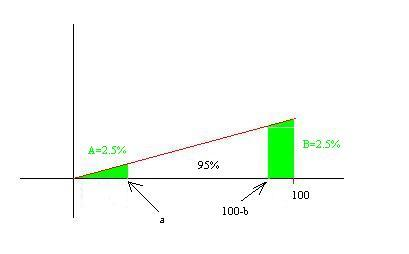
\includegraphics[width=8cm]{Graphs/Graph_HW4.jpg}
\end{center}
\caption{Density of $T_0$ \label{FIGHW4}}
\end{figure}
In order to determine a 95\% confidence interval, we can e.g.\ truncate 2.5\% on the left and the right side, respectively, as indicated in Fig.\ \ref{FIGHW4}. We have:
\begin{eqnarray*}
0.025 = A &=& \frac{1}{2}\,a \, f_{0}(a) \\
\Rightarrow 0.025 &=& \frac{1}{2} a\frac{2a}{10,000}\\
\Rightarrow a^2 &=& 250 \\
\Rightarrow a &\approx& 15.8113883\\
\end{eqnarray*}
and
\begin{eqnarray*}
0.025 = B &=&\underbrace{\frac{1}{2} b \, \left(f_{0}(100) - f_{0}(100-b)\right)}_{\text{upper part}} + \underbrace{b\,f_{0}(100-b)}_{\text{bottom part}} \\
\Rightarrow 0.025 &=& \frac{1}{2} b f_{0}(100) + \frac{1}{2} b f_{0}(100-b) \\
\Rightarrow 0.025 &=& \frac{1}{2} b \frac{2\cdot 100}{10,000}m + \frac{1}{2}\frac{2\cdot (100-b)}{10,000} \\
&=& \frac{2\cdot b}{100} - \frac{b^2}{10,000}\\
\stackrel{\text{quad. form.}}{\Rightarrow} b &=& \frac{-\frac{2}{100}+\sqrt{\frac{4}{100} - \frac{1}{100,000}}}{\frac{-2}{10,000}}\\
&=& 1.25791171. 
\end{eqnarray*}
Therefore, $[a,100-b] = [15.8113883,98.74208829]$ is a 95\% confidence interval \textbf{for one life}.

For 100 lives with lifetimes $T^i_0$, $1\leq i \leq 100$, use the Central Limit Theorem:
\begin{eqnarray*}
\lim_{n\rightarrow \infty} P\left( \frac{\sum_{i=1}^n T^i_0 - n \stackrel{\circ}{e}_{0} }{\sigma_{T_0} \sqrt{n}} \leq z\right) &=& \Phi(z)\\
\text{or }
\lim_{n\rightarrow \infty} P\left( \frac{\sum_{i=1}^n T^i_0}{n} \leq \stackrel{\circ}{e}_{0} 
+ z \, \frac{\sigma_{T_0}}{\sqrt{n}} \right) &=& \Phi(z),
\end{eqnarray*}
so a 95\% (asymptotic) confidence interval is given by
$$
\left[\stackrel{\circ}{e}_{0} - \underbrace{1.960}_{=z_{0.975}} \, \frac{\sigma_{T_0}}{\sqrt{100}},\stackrel{\circ}{e}_{0} + \underbrace{1.960}_{=z_{0.975}} \, \frac{\sigma_{T_0}}{\sqrt{100}} \right] \approx [62.046956,71.286386].
$$

\item We have
\begin{eqnarray*}
\stackrel{\circ}{e}_{1:\overline{1.5}|} &=& \int_0^{1.5} {_tp_1}\,dt = \int_0^{1} {_tp_1}\,dt + \int_1^{1.5} {_tp_1}\,dt =  \int_0^{1} 1- t\cdot {q_1}\,dt + {p_1}\,\int_1^{1.5} {_{t-1}p_2}\,dt \\
&\stackrel{s=t-1}{=}&  1- {q_1}\, \int_0^{1} t\,dt + {p_1}\,\int_0^{0.5} {_{s}p_2}\,ds  = 1 - {q_1}\, \left[0.5\cdot t^2\right]_{t=0}^1 + {p_1}\, \int_0^{0.5} 1 - s\cdot {q_2}\,ds\\
&=& 1 -  0.5\cdot q_1 + {p_1}\,\left(\left[s - {q_2}\cdot 0.5\cdot s^2\right]_{s=0}^{0.5}\right) =
0.95 + 0.9\,\left(0.5 - 0.05\cdot 0.5 \cdot 0.5^2\right) = 1.394375.
\end{eqnarray*}
\item We have
\begin{eqnarray*}
\stackrel{\circ}{e}_0 &=& \int_0^{\omega} {_tp_0}\,dt = \int_0^{\omega} S_0(t)\,dt = \int_0^{\omega} (1-t/\omega)^{\alpha}\,dt \\
&=& \left[-\frac{\omega}{\alpha+1} \left(1 - t/\omega\right)^{\alpha+1}\right]_{t=0}^{\omega} = \frac{\omega}{\alpha+1}.
\end{eqnarray*}
Let us now denote the previous quantities by ``$\cdot_P$" and the new quantities by ``$\cdot_N$". Then, the first point yields
$$
\frac{\omega}{\alpha_N + 1} = 1/2 \cdot \frac{\omega}{\alpha_P + 1} \;\; \Rightarrow \;\; \alpha_N = 2\cdot \alpha_P + 1.
$$
Moreover, since the force of mortality is
$$
\mu_x = \frac{-S_0'(x)}{S_0(x)} = \frac{\alpha/\omega\cdot (1-x/\omega)^{\alpha-1}}{(1-x/\omega)^\alpha} = \frac{\alpha}{\omega - x},
$$
by b.\ we obtain
$$
\frac{\alpha_N}{\omega- x} = 2.25\cdot \frac{\alpha_P}{\omega- x} \;\; \Rightarrow \;\; \alpha_N = 2.25 \cdot \alpha_P.
$$
Thus,
$$
2.25 \cdot \alpha_P = 2\cdot \alpha_P + 1 \;\; \Rightarrow \;\; 0.25\cdot \alpha_P = 1 \;\; \Rightarrow \;\; \alpha_P = 4. 
$$

\item
We need to solve:
$$
{_{m(x)}p_x} = 0.5.
$$
1st Observation:
$$
t \mapsto {_tp_x} \text{ is a decreasing function}.
$$
2nd Observation:
$$
{_tp_x} \text{ are available for discrete }t.
$$
Let $[m(x)]$ be the greatest integer smaller or equal to $m(x)$. Then, due to the 1st observation, we have
$$
{_{[m(x)]}p_x}  \geq \underbrace{{_{m(x)}p_x}}_{=0.5}  > {_{[m(x)]+1}p_x},
$$
i.e.\ we can determine $[m(x)]$ by looking for the ages where ${_{[m(x)]}p_x} $ is greater or equal, but  ${_{[m(x)]+1}p_x} $ is smaller than 0.5. Thus, we obtain
$$
[m(0)] = 77 \text{ and } [m(50)] = 29.
$$
Now:
\begin{eqnarray*}
0.5 &\stackrel{!}{=}& {_{m(x)}p_x} = {_{[m(x)]}p_x}\cdot {_{m(x)-[m(x)]}p_{x+[m(x)]}}\\
&\stackrel{\text{unif.\ dist.}}{=}&   {_{[m(x)]}p_x} \left( 1- (m(x)-[m(x)])\cdot{q_{x+[m(x)]}}\right)\\
\Rightarrow m(x) &=& \frac{1 -\frac{0.5}{_{[m(x)]}p_x}}{q_{x+[m(x)]}} + [m(x)]\\
\Rightarrow m(0) &\approx& 77.59\\
\text{and }  m(50) &\approx& 29.15.
\end{eqnarray*}
\end{enumerate}

\normalsize

\subsection*{Constant Force of Mortality over the Year}

Alternatively, we may assume that the force of mortality remains constant over the year:
\begin{eqnarray*}
&& p_x = e^{-\int_0^1 \mu_{x+t}\,dt} = e^{-\mu_x},\\
&\text{where }& \mu_{x+t} = \mu_{x},\;0 \leq t < 1\\
&\Rightarrow& \mu_{x+t} = \mu_x = -\log\left\{p_x\right\},\;0 \leq t < 1 \\
&\text{and, hence, }& {_tp_x} = e^{-\int_0^t \mu_{x+t}\,dt} = e^{-\mu_x\,t} = p_x^t.
\end{eqnarray*}
This, on the other hand, implies:
\begin{eqnarray*}
&& \frac{S_0(x+t)}{S_0(x)} = \left(\frac{S_0(x+1)}{S_0(x)}\right)^t \\
&\Rightarrow& S_0(x+t) = S_0(x)\left(\frac{S_0(x+1)}{S_0(x)}\right)^t,\;0\leq t < 1,
\end{eqnarray*}
so we are looking at an \textbf{exponential interpolation} scheme.

Clearly, all other quantities can now again be derived on the basis of $s(x+t)$ (see Homework \ref{HW5}). In particular, for the integral we obtain
\begin{eqnarray*}
\int_0^1 {_tp_x}\,dt &=& \int_0^1 p_x^t\,dt = \left[\frac{p_x^t}{\log\left\{p_x\right\}}\right]_{t=0}^{1} \\
&=& \frac{p_x^t - 1}{\log\left\{p_x\right\}}
\end{eqnarray*}
So, for instance, if $p_x = .98$, then $\int_0^1 {_tp_x}\,dt = .989966$.

\subsection*{Balducci Assumption}
The Balducci assumption supposes a \textbf{hyperbolic interpolation} scheme on $s(x)$, i.e.\
$$
\frac{1}{S_0(x+t)} = \frac{1}{S_0(x)} + t\left(\frac{1}{S_0(x+1)} -\frac{1}{S_0(x)} \right).
$$ 
This yields
$$
{_tp_x} = \frac{S_0(x+t)}{S_0(x)} = \left(1 + t(\frac{1}{p_x} - 1)\right)^{-1} = \frac{p_x}{p_x + t(1-p_x)},
$$
and similarly, we can make use of this interpolation scheme to derive all other quantities of interest.

For the integral, in this case, we have
\begin{eqnarray*}
\int_0^1 {_tp_x}\,dt &=& \int_0^1 \frac{p_x}{p_x + t(1-p_x)}\,dt = p_x \cdot \left[\frac{\log\left\{p_x + t(1-p_x)\right\}}{1-p_x}\right]_{t=0}^{1} \\
&=& \frac{p_x}{p_x - 1} \log\{p_x\}.
\end{eqnarray*}
So, for instance, if $p_x = .98$, then $\int_0^1 {_tp_x}\,dt = .989933$.

\begin{homework}
\label{HW8}
\begin{enumerate}
\item For the assumption of a constant force of mortality and the hyperbolic assumption, determine $_tq_x$, $\mu_{x+t}$, $_{1-t}q_{x+t}$, $_{u}q_{x+t}$, $_tp_x$, and ${_tp_x}\,\mu_{x+t}$ for $0\leq t <1$ and $0 \leq u \leq 1-t$.
\item If $q_{70}=0.04$ and $q_{71}=0.05$, calculate the probability that that (70) will die between ages $70\frac{1}{2}$ and $71\frac{1}{2}$ under\footnote{This is Problem 3.30 in \cite{BOWERS}.} 
\begin{enumerate}
\item The assumption that deaths are uniformly distributed within each year of age.
\item The hyperbolic assumption for each year of age. 
\end{enumerate} 
\item What is the order of $\int_0^1 {_tp_x}\,dt$ for the different schemes? Why is it ``implied by the different interpolation schemes"? Give a short explanation. 
\end{enumerate}
\end{homework}

\noindent \textbf{Solution} to Homework \ref{HW8}:
\footnotesize 
\begin{enumerate}
\item
\begin{itemize}
\item \textit{Constant Force of Mortality:}

We know from above for $0\leq t \leq 1$
\begin{eqnarray*}
\mu(x+t) &=& \log\{p_x\} \\
\text{and } {_tp_x}&=& {p_x}^t \\
\Rightarrow {_tq_x} &=& 1 - {_tp_x} = 1 - {p_x}^t.
\end{eqnarray*}
Therefore, we have
\begin{eqnarray*}
{_tp_x}\,\mu(x+t) &=& -{p_x}^t \, \log\{p_x\} \\ 
\text{and } {_{y}p_{x+t}} & =& \exp\left\{\int_{x+t}^{x+t+y}-\mu(s)\,ds\right\}\\
&=& \exp\left\{\log\{p_x\}\,\int_{x+t}^{x+t+y}\,ds\right\} = \exp\left\{\log\{p_x\}\,y\right\}\\
&=& {p_x}^{y},
\end{eqnarray*}
where $0\leq y \leq 1-t$. Thus,
$$
{_yq_{x+t}} = 1 - {p_x}^y,
$$
and for $y=1-t$, we have
$$
{_{1-t}q_{x+t}} = 1 - {p_x}^{1-t}.
$$

\item \textit{Balducci Assumption:}

From above we know
\begin{eqnarray*}
{_tp_x} &=& \frac{p_x}{{p_x} + t(1-{p_x})} = \frac{p_x}{1-{q_x} + t \,{q_x}}\\
&=& \frac{p_x}{1- (1-t)\,{q_x}}\\
\Rightarrow {_tq_x} &=& 1 - {_tp_x} = 1 -  \frac{p_x}{1- (1-t)\,{q_x}}\\
&=&  \frac{1- (1-t)\,{q_x} - {p_x}}{1- (1-t)\,{q_x}} = \frac{1- {q_x} + t\,{q_x} - 1 + {q_x}}{1- (1-t)\,{q_x}} \\
&=&  \frac{t\,{q_x}}{1- (1-t)\,{q_x}}.
\end{eqnarray*}
And thus,
\begin{eqnarray*}
\mu(x+t) = \frac{-s'(x+t)}{s(x+t)} &=& \frac{-\frac{\partial}{\partial t} {_{x+t}p_0}}{{_{x+t}p_0}}
=  \frac{-\frac{\partial}{\partial t} \left({_xp_0}\cdot{_{t}p_x}\right)}{{_xp_0}\cdot{_{t}p_x}} \\
&=&   \frac{-{_xp_0}\frac{\partial}{\partial t} \left({_{t}p_x}\right)}{{_xp_0}\cdot{_{t}p_x}} 
=   \frac{-\frac{\partial}{\partial t} \left({_{t}p_x}\right)}{{_{t}p_x}}
\end{eqnarray*}
\begin{eqnarray*}
&=& \frac{-\frac{\partial}{\partial t} \left(\frac{p_x}{1- (1-t)\,{q_x}}\right)}{\frac{p_x}{1- (1-t)\,{q_x}}}
= \frac{-\frac{\partial}{\partial t} \left(\frac{1}{1- (1-t)\,{q_x}}\right)}{\frac{1}{1- (1-t)\,{q_x}}}\\
&=& \frac{\frac{q_x}{\left(1- (1-t)\,{q_x}\right)^2}}{\frac{1}{1- (1-t)\,{q_x}}}
= \frac{{q_x}}{1- (1-t)\,{q_x}},
\end{eqnarray*}
and, hence,
$$
{_tp_x}\, \mu(x+t) = \frac{{q_x}\cdot{p_x}}{\left(1- (1-t)\,{q_x}\right)^2}.
$$
 Moreover, for  $0\leq y \leq 1-t$
 \begin{eqnarray*}
 {_yq_{x+t}} &=& \frac{S_0(x+t) - S_0(x+t+y)}{S_0(x+t)} \\
 %&=& \frac{\frac{1}{\frac{1}{s(x)} + t\left(\frac{1}{s(x+1)} - \frac{1}{s(x)}\right)} - \frac{1}{\frac{1}{s(x)} + (t+y)\left(\frac{1}{s(x+1)} - \frac{1}{s(x)}\right)}}{\frac{1}{\frac{1}{s(x)} + t\left(\frac{1}{s(x+1)} - \frac{1}{s(x)}\right)}}
 &=& \frac{{_{x+t}p_0} - {_{x+t+y}p_0}}{{_{x+t}p_0}} = \frac{{_{x}p_0}\left({_{t}p_x} - {_{t+y}p_x}\right)}{{_{x}p_0}\cdot{_{t}p_x}} \\
 &=& \frac{\frac{p_x}{1- (1-t)\,{q_x}} - \frac{p_x}{1- (1-t-y)\,{q_x}}}{\frac{p_x}{1- (1-t)\,{q_x}} }
 = 1 - \frac{1- (1-t)\,{q_x}}{1- (1-t-y)\,{q_x}}\\
 &=& \frac{1- (1-t-y)\,{q_x} -1+ (1-t)\,{q_x}}{1- (1-t-y)\,{q_x}}
 = \frac{y\,{q_x}}{1- (1-y-t)\,{q_x}}
 \end{eqnarray*}
 and for $y=1-t$:
$$
 {_{1-t}q_{x+t}} = \frac{(1-t)\,{q_x}}{1- (1-1 + t-t)\,{q_x}} = (1-t)\,{q_x}.
 $$
\end{itemize}

\item Note that this is not the probability that (70.5) will die between 70.5 and 71.5, but that (70) will die between 70.5 and 71.5.

The first probability is
\begin{eqnarray*}
{q_{70.5}} &=& 1 - {p_{70.5}}\\
&=& 1 - {_{0.5}p_{70.5}}\cdot{_{0.5}p_{71}} \\
&=& 1 - ( 1 - {_{0.5}q_{70.5}})(1 - {_{0.5}\cdot q_{71}}),
\end{eqnarray*}
and, therefore:
\begin{itemize}
\item Unif.\ Dis.:
\begin{eqnarray*}
{q_{70.5}} &=& 1 - ( 1 - \frac{0.5\,{q_{70}}}{1 - 0.5 \, q_{70}})(1 - {0.5}\,{q_{71}})\\
&=& 0.04489,
\end{eqnarray*}
\item Balducci:
\begin{eqnarray*}
{q_{70.5}} &=& (1 - 0.5\,q_{70}) \frac{1- q_{71}}{1 - 0.5 q_{71}}\\
&=& 0.045128.
\end{eqnarray*}
\end{itemize}
\item Comparison: From the examples above, we see that there are only slight differences in the value of the integral between the different cases. However, the order of the different schemes  actually is implied by the different interpolation methods as can be seen from Figure \ref{FIGFRACAGE}.
\begin{figure}
\begin{center}
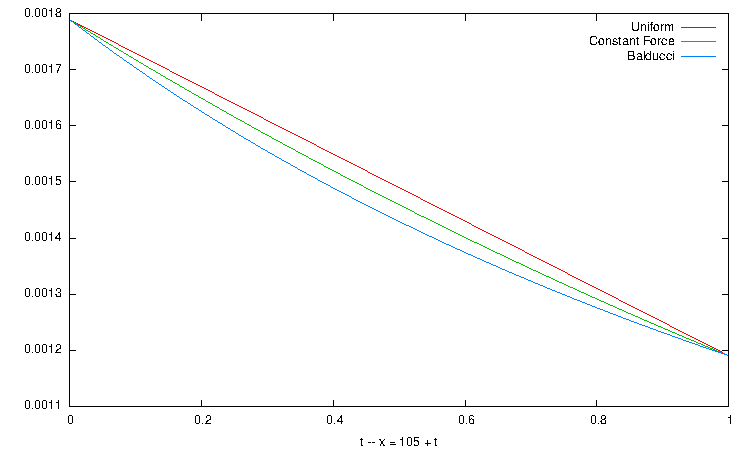
\includegraphics[width=8cm]{Graphs/Graph_Interpolatiomethods.pdf}
\end{center}
\caption{Assumptions for fractional ages \label{FIGFRACAGE}}
\end{figure}
We see that for the survival function $s$, we have the following order: 
$$
 \text{Unif.\ Dis. } > \text{ Const.\ Force } > \text{ Balducci}.
$$
Since integration preserves the order, we will have the same order for $\int_0^1 {_tp_x}\,dt$.
\end{enumerate}
\normalsize

\section{Analytic Mortality Laws}
\label{SECANALML}
While their use in actuarial practice for modeling (human) life contingencies is limited, \textit{Analytic Mortality Laws}, i.e.\ analytic survival or mortality functions, still have their justification. For example, they provide simple approximations or they can be used when modeling the decay of other phenomena. 

A survival function $S_0$ has the properties $S_0(0)=1$ and $\lim_{x\rightarrow \infty} S_0(x) = 0$. Thus, the simplest approach when imposing some limiting age $\omega$, implying $S_0(\omega)=0$, is to simply connect the points $(0,1)$ and $(\omega,0)$ by a straight line. This is the \textit{De Moivre Mortality Law}:
$$
S_0(x) = 1 - \frac{x}{\omega},\;0 \leq x \leq \omega.
$$
The force of mortality in this case is given by
$$
\mu_x= \frac{-S_0'(x)}{S_0(x)} = \frac{\frac{1}{\omega}}{1 - \frac{x}{\omega}} = \frac{1}{\omega - x},\;0 \leq x < \omega.
$$
The \textit{generalized De Moivre Law} corresponds to a survival function of the form
$$
S_0(x) = \left(1 - \frac{x}{\omega}\right)^{\alpha},\;0\leq x \leq \omega,\;\alpha>0.
$$
Here,
$$
\mu_x = \frac{\alpha/\omega\,(1-x/\omega)^{\alpha-1}}{(1-x/\omega)^{\alpha}} = \frac{\alpha}{\omega - x},\;0\leq x \leq \omega.
$$

A slightly more advanced approach is to impose a structure on the force of mortality, where the properties in Section \ref{CURLIFTFORC} must be satisfied. The simplest example in this category is a constant force of mortality $\mu$, which corresponds to an Exponentially distributed lifetime $T_x$, i.e.\
$$
S_0(x) = e^{-\mu\,x}.
$$
However, here the force of mortality does not increase with the age; therefore, its application for modeling human mortality is problematic.

\cite{GOMPERTZ} proposed to use an exponential function:
$$
\mu_x = B\cdot c^x,\,B>0,\,c>1,\,x\geq 0
$$
implying a survival function of the form (cf. Homework \ref{HW4})
$$
S_0(x) = \exp\left\{ - \frac{B}{\log(c)} (c^x - 1)\right\}. 
$$
This mortality law is called the \textit{Gompertz Mortality Law}.

\cite{MAKEHAM} proposed to add an age-independent term into the Gompertz form due to external causes of death:
$$
\mu_x = A + B\cdot c^x,\,B>0,\,A\geq -B,\,c>1,\,x\geq 0.
$$
Then, for the survival function, we have:
\begin{eqnarray*}
S_0(x) &=& {_xp_0} = \exp\left\{-\int_0^x \mu_t\,dt\right\}\\
&=& \exp\left\{-\int_0^x A\,dt\right\}\,\exp\left\{-\int_0^x B\cdot c^t\,dt\right\}\\
&\stackrel{\text{Homew.\ \ref{HW4}}}{=} & \exp\{-A x\}\,\exp\left\{ - \frac{B}{\log(c)} (c^x - 1)\right\} \\
&=& \exp\left\{ - Ax - \frac{B}{\log(c)} (c^x - 1)\right\}
\end{eqnarray*}
This mortality law is called the \textit{Gompertz-Makeham} or \textit{Makeham Mortality Law}.

Another approach frequently used in lifetime analysis is the so called \textit{Weibull} law:
$$
\mu_x = kx^n,\,k>0,\,n>0.
$$
By Homework \ref{HW4},  
$$
S_0(x) = \exp\left\{ - \frac{k}{n+1} x^{n+1}\right\}.
$$

Homework \ref{HW9} provides a simple example of the application of such a mortality law for modeling the decay of buildings taken from the MLC Exam Spring 2007 (Problem 21).

\begin{homework}
\label{HW9}
\begin{enumerate}
\item You are given the following information about a new model for buildings with limiting age $\omega$.
\begin{enumerate}
\item The expected number of buildings surviving at age $x$ will be
$$
l_x = \left(\omega - x\right)^{\alpha},\,x<\omega.
$$ 
\item The new model predicts a $33\frac{1}{3}\%$ higher complete life expectancy (over the previous De Moivre model with the same $\omega$) for buildings aged 30.
\item The complete life expectancy for buildings aged 60 under the new model is 20 years.
\end{enumerate}
Calculate the complete life expectancy under the previous De Moivre model for buildings aged 70.
\end{enumerate}
\end{homework}

\textbf{Solution} to Homework \ref{HW9}:

\footnotesize
\begin{enumerate}
\item First:
$$
0.20 = {_2p_x} = p_x\,p_{x+1} = e^{-\mu_x}\,e^{-\mu_{x+1}} = e^{-\mu_x}\,e^{-2\,\mu_x} = e^{-3\,\mu_x} 
$$
so that
$$
\mu_x = - \frac{\log\{0.20\}}{3} = 0.53648.
$$
Now:
\begin{eqnarray*}
{_{0.25|1.5}q_x} &=& {_{0.25}p_x} - {_{1.75}p_x} = e^{-0.25\,\mu_x} - e^{-\mu_x}\,e^{-0.75\,\mu_{x+1}} \\
&=& e^{-0.25\,\mu_x} - e^{-\mu_x}\,e^{-0.75\,2\,\mu_x} =  e^{-0.25\,\mu_x} - e^{-2.5\,\mu_x} = 0.61295.\\
\Rightarrow {_{1.5}q_{x+0.25}} &=& \frac{{_{0.25|1.5}q_x}}{_{0.25}p_x} = \frac{0.61295}{e^{-0.25\,\mu_x}}= 0.70093.
\end{eqnarray*}
\item We have:
\begin{eqnarray*}
\stackrel{\circ}{e}^{\text{NEW}}_x &=& \int_0^{\infty} {_tp_x}\,dt 
= \int_0^{\infty} \frac{l_{x+t}}{l_x} \,dt\\
&=& \frac{1}{(\omega - x)^{\alpha}} \int_0^{\omega - x} (\omega - x - t)^{\alpha}\,dt
= \frac{1}{(\omega - x)^{\alpha}} \left[\frac{-1}{\alpha + 1} (\omega - x - t)^{\alpha+1}\right]_{t=0}^{t=\omega - x}\\
&=& \frac{\omega - x}{\alpha + 1}
\end{eqnarray*}
and 
\begin{eqnarray*}
\stackrel{\circ}{e}^{\text{OLD}}_x  &=& \int_0^{\infty} {_tp_x}\,dt 
= \int_0^{\infty} \frac{S_0(x+t)}{S_0(x)} \,dt\\ 
&=& \frac{1}{1 - \frac{x}{\omega}} \int_0^{\omega - x} 1 - \frac{x+t}{\omega}\,dt
= \frac{1}{1 - \frac{x}{\omega}} \left(\left[t\right]_{t=0}^{t=\omega - x} - \left[\frac{1}{2\omega}(x+t)^2\right]_{t=0}^{t=\omega - x}\right)\\
&=& \frac{\omega^2 - 2\omega x + x^2}{2(\omega - x)}
= \frac{\omega - x}{2}.
\end{eqnarray*}
From condition (ii), we obtain
\begin{eqnarray*}
\underbrace{\frac{\omega - 30}{\alpha + 1}}_{=\stackrel{\circ}{e}^{\text{NEW}}_{30}} \stackrel{!}{=} \underbrace{\frac{4}{3} \frac{\omega - 30}{2}}_{=\stackrel{\circ}{e}^{\text{OLD}}_{30}}
\Rightarrow \underbrace{\frac{\omega - 30}{\alpha + 1}}_{=\stackrel{\circ}{e}^{\text{NEW}}_{30}} \stackrel{!}{=} \underbrace{\frac{\omega - 30}{1.5}}_{=\stackrel{\circ}{e}^{\text{OLD}}_{30}}
\Rightarrow \alpha = 0.5,
\end{eqnarray*}
and from (iii)
$$
\frac{\omega - 60}{1.5} = 20 \Rightarrow \omega = 90.
$$
Thus,
$$
\stackrel{\circ}{e}^{\text{OLD}}_{70} = \frac{90-70}{2} = 10.
$$
\end{enumerate}
\normalsize

\section{Select and Ultimate Tables}
\label{SECSELULTTABS}
 
 In actuarial practice, tables are compiled for different cohorts, i.e.\ different parts of the population which are assumed to have a similar risk of dying. For example, usually males and females or smokers and non-smokers are distinguished. However, gender or smoking habits are not the only information that should be taken into account in the calculation of an insurance policy; the duration of the contract is another important risk factor.
 
Consider two persons, $(55)$ and $(55)^*$, who both are 55-year old male non-smokers holding an insurance contract. However, while $(55)$ underwrote his contract thirty years ago at the age of 25, $(55)^*$ just recently concluded his contract, and for both of them it was necessary to pass a mandatory health examination in order to be eligible for the purchase. For the death probability at age 55 for $(55)$, $q_{55}^{(55)}$, the health examination some thirty years ago does not present any additional information. The recent health examination of $(55)^*$, on the other hand, certainly does: We know for sure that $(55)^*$ does not have diabetes, cancer, or another disease since he ``passed" the health examination, but we cannot make the same inference about $(55)$. Thus, the death probability for $(55)^*$ at 55, $q_{55}^{(55)^*}$, will be lower:
$$
{q_{55}^{(55)^*}} < {q_{55}^{(55)}}.
$$
In contrast, for the death probability at age 85, i.e.\ thirty years later, the mandatory health examination usually does  not present a considerable information gain, since both health examinations took place a long time ago. Therefore, here it is adequate to assume:
$$
{q_{85}^{(55)^*}} = {q_{85}^{(55)}} = {q_{85}}.
$$
The latter death probability can hence be drawn from a life table ``as we are used to", whereas in the prior probabilities, selection effects have to be taken into account:
\begin{eqnarray*}
{q_{55}^{(55)^*}} = q_{[55]} &\neq& q_{55} = q_{[25]+30} =   {q_{55}^{(55)}},\\
{q_{85}^{(55)^*}} = q_{[55]+30} &=& q_{85} = q_{[25]+60} =   {q_{85}^{(55)}}.
\end{eqnarray*}
Here, the bracketed $[55]$ and $[25]$ denote the age at selection. Now, $q_{[x]+i}$, $i=0,1,2,...$ are drawn from so-called \textit{select tables}, whereas $q_{[x]+i} = q_{x+i}$ for $i=30,31,...$ are drawn from an \textit{ultimate table}. In this example, we have a selection period of $30$ years, but in general it may be more or less. For a selection period of $r$ years, we have:
\begin{itemize}
\item $i \geq r$
\begin{eqnarray*}
q_{[x]+i} &=& q_{x+i};\\
p_{[x]+i} &=& p_{x+i};\\
l_{[x]+i} &=& l_{x+i}.
\end{eqnarray*}
\item $i < r$:

Here, our usual formulas still hold, but we have to consider the different cohorts:
\begin{eqnarray*}
l_{[x]} \cdot \underbrace{(1-q_{[x]})}_{p_{[x]}} &=& l_{[x]+1}; \\
l_{[x]+1} \cdot \underbrace{(1-q_{[x]+1})}_{p_{[x]+1}} &=& l_{[x]+1};\\
&...&\\
l_{[x]+r-1} \cdot \underbrace{(1-q_{[x]+r-1})}_{p_{[x]+r-1}} &=& l_{[x]+r} = l_{x+r};\\
l_{x+r} \cdot \underbrace{(1-q_{x+r})}_{p_{x+r}} &=& l_{x+r+1}; \\
&...&
\end{eqnarray*}
and 
$$
{_tp_{[x]+i}} = \frac{l_{[x]+i+t}}{l_{[x]+i}}.
$$
\end{itemize}

\begin{figure}
\begin{center}
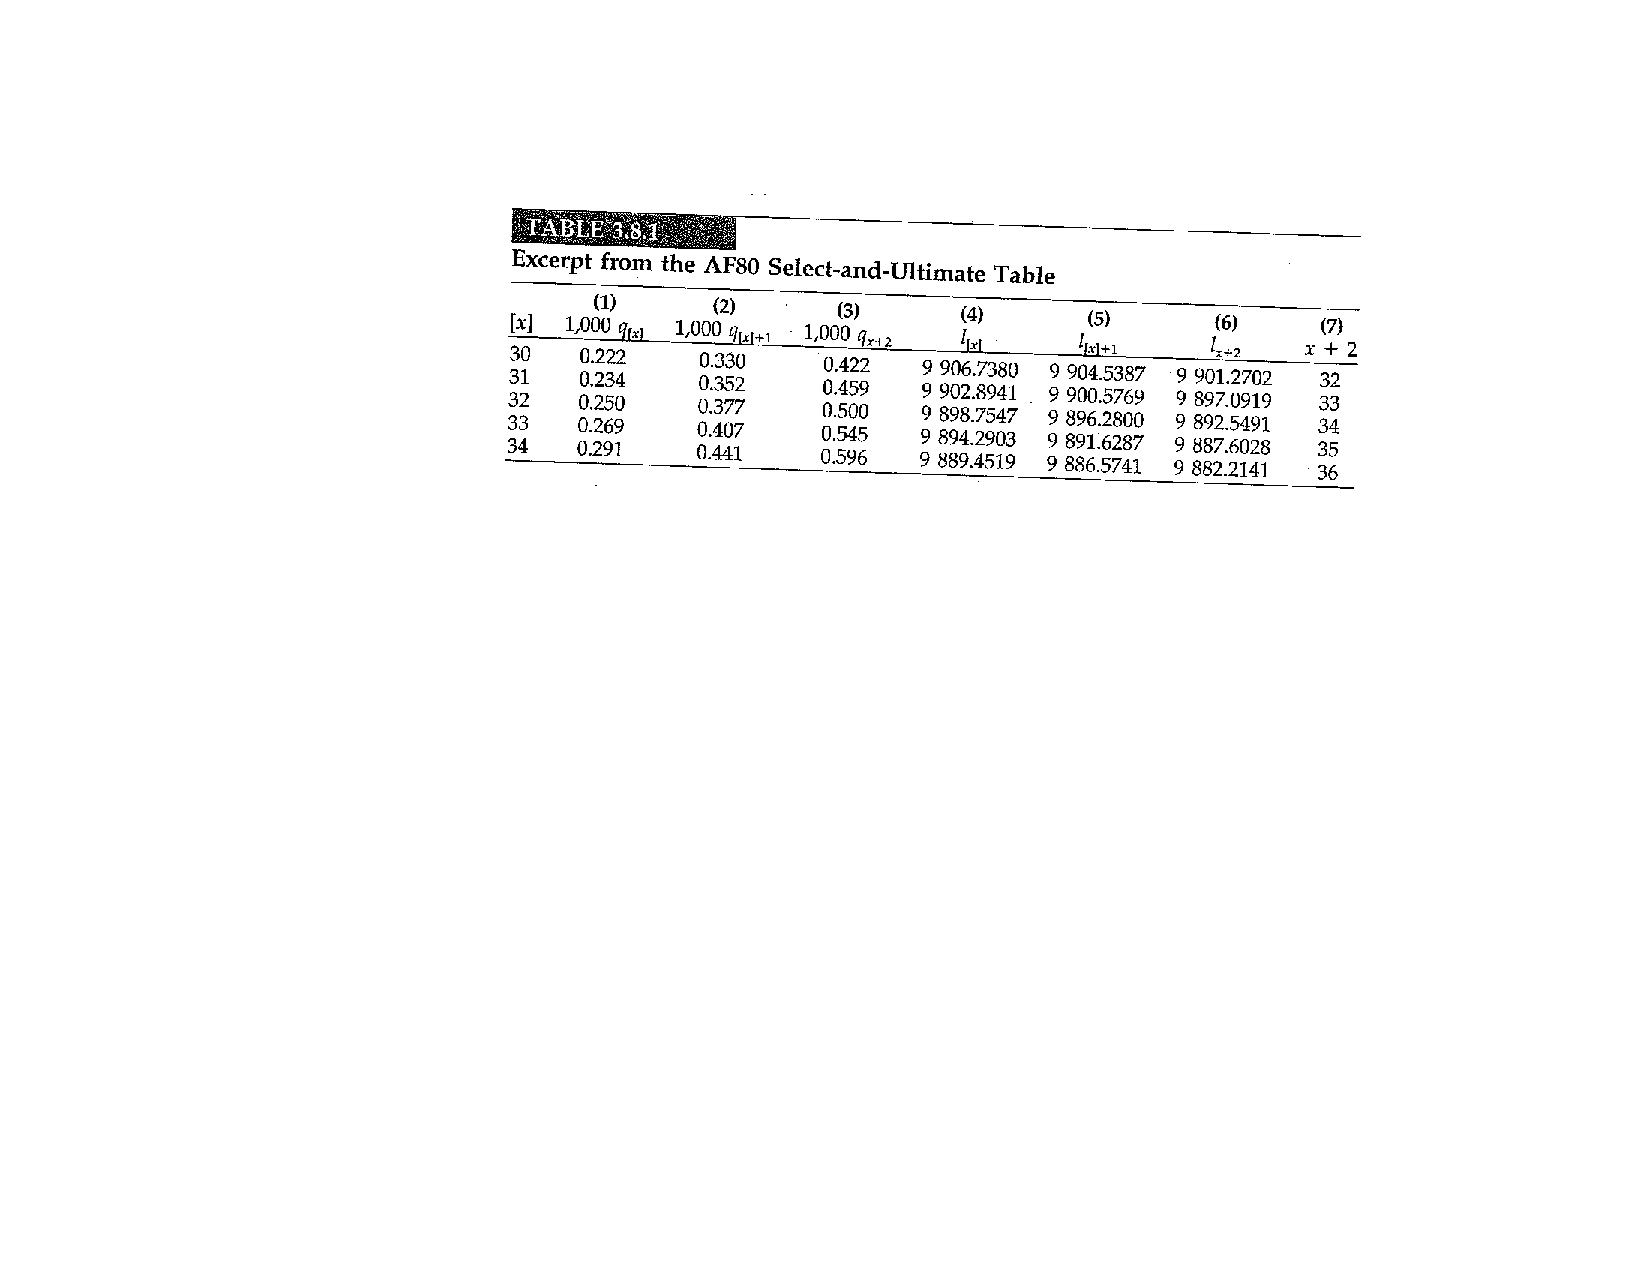
\includegraphics{Graphs/Select.pdf}
\end{center}
\caption{Select-and-Ultimate table from \cite{BOWERS} \label{FIGSELUL}}
\end{figure}

As an example, in Figure \ref{FIGSELUL} a Select-and-Ultimate table is displayed with a selection period $r=2$. The first $r$ columns ((1), (2) and (4), (5), respectively) are the selection part, whereas the $r+1st$ column ((3) and (6), respectively) present the ultimate part. The evolution of each cohort can be followed by first going to the right, e.g.
$$
l_{[30]} \rightarrow l_{[30]+1} \rightarrow l_{[30]+2} = l_{32}
$$
and then down as usual
\begin{eqnarray*}
&& l_{32}\\
&\rightarrow& l_{33} \\
&&...
\end{eqnarray*}

\begin{exercise}
Based on this table, calculate
\begin{eqnarray*}
{_5p_{[30]}} &=& \frac{l_{[30]+5}}{l_{[30]}} = \frac{l_{35}}{l_{[30]}} \\
&=& \frac{9,887.6028}{9,906.7380} = .99807.
\end{eqnarray*}
\begin{eqnarray*}
{_3q_{[31]+1}} &=& \frac{l_{[31]+1} - l_{[31]+1+3}}{l_{[31]+1}} =\frac{l_{[31]+1} - l_{35}}{l_{[31]+1}}\\
&=& \frac{9,900.5769 - 9,887.6028}{9,900.5769} = .00131.
\end{eqnarray*}
\end{exercise}

\chapter{Life Insurance}
\label{CHAPLIFEINSURANCE}

In our introductory example from Section \ref{SECINEXAM}, we introduced a first life insurance contract, namely a \textit{pure endowment contract} delivering a fixed payment upon survival until a certain point in time. We pointed out that the contract's payoff is a random variable depending on the survival of Mr.\ (55) until the age of 70,  but we also found that the interest rate is important, too, as we are considering future payments.

In reality, interest rates evolve stochastically. However, certain financial instruments are available, so-called zero-coupon or discount bonds, which provide the present value of a dollar paid at some future point in time $t$, i.e.\ they define a \textbf{discount function} of future payments
$$
v_{\cdot}: \left[0,\infty \right) \longrightarrow [0,1],\;t \mapsto v_t.
$$
Hence, the present value of a future \textbf{benefit} at time $t$, $b_t$, is
$$
z_t = v_t \cdot b_t.
$$
In order to simplify notation, here we assume constant \textit{rate of interest} $i$ or, equivalently, a constant \textit{force of interest} $\delta$. Clearly, we have
\begin{eqnarray*}
e^{\delta} = 1 + i &\Rightarrow& i = e^{\delta} - 1,\\
&\Rightarrow& \delta = \log\left\{1+i \right\},
\end{eqnarray*}
and for the discount function we have
$$
v_t = e^{-\delta \cdot t} = \left(\frac{1}{1+i}\right)^t = v^t,
$$
where
\begin{eqnarray*}
v = v_1 = \frac{1}{1+i} = e^{\delta} &\Rightarrow& i = \frac{1}{v} - 1\\
&\Rightarrow&  \delta = - \log\left\{v\right\}.
\end{eqnarray*}

Hence, the present value of every dollar of Mr.\ (55)'s 15-year endowment contract is 
$$
v_{15} = v^{15}, 
$$
but only if he is alive on his 70th birthday! Thus, the present value is contingent on his \textbf{remaining lifetime}, $T_{55}$:
\begin{itemize}
\item If $T_{55} \leq 15$, i.e.\ if his future lifetime is less than 15 years, he will die before 70, and the discounted payoff will be
$$
z_{15} = v^{15}\cdot 0 = 0.
$$
\item If $T_{55}>15$, i.e.\ if his future lifetime exceeds 15 years, he will be alive at 70, and the discounted payoff will be
$$
z_{15} = v^{15} \cdot 1 = v^{15}.
$$
\end{itemize}
Thus, the present value is a random variable ($\rightarrow$ the \textit{present value random variable}) contingent on his survival:
$$
Z = \left\{
\begin{array}{c l}
0 & ,\text{ if }_{55} \leq 15 \\
v^{15} &, \text{ if }T_{55} > 15
\end{array}
\right. .
$$
or, for a general $n$-year pure endowment contract paying one dollar at the end of $n$ years if and only if the $x$-year old insured survives at least $n$ years from the time of policy issue:
$$
Z = \left\{
\begin{array}{c l}
0 & ,\text{ if }T_x \leq n \\
v^{n} &, \text{ if }T_x > n
\end{array}
\right.
$$

For Mr.\ (55), we further found that the expected discounted amount at his disposal, i.e.\ per dollar
\begin{eqnarray*}
E[Z] &=& E\left[v^{15}\, 1_{\left\{T_{55} > 15\right\}} + 0\, 1_{\left\{T_{55} \leq 15 \right\}}\right] = v^{15}\,E\left[1_{\left\{T_{55} > 15\right\}} \right] \\
&=& v^{15}\, Pr\left(T_{55} > 15 \right) 
= v^{15}\,{_{15}p_{55}},
\end{eqnarray*}
coincides with the amount he pays initially, i.e.\ the (single upfront) premium in a scheme with infinitely many insureds. We will come back to this observation later in the course. 

In general, for an $n$-year pure endowment we have for the \textbf{expected present value of future benefits} (the \textbf{actuarial present value}):
\begin{eqnarray}
A_{x:\stackrel{1}{\overline{n\,}|}} &=& E[Z] 
=  E\left[v^{n}\, 1_{\left\{T_x > n\right\}} + 0\, 1_{\left\{T_x \leq n \right\}}\right] \nonumber \\
&=& v^{n}\,E\left[1_{\left\{T_x > n\right\}} \right]  
= v^{n}\, Pr\left(T_x > n \right)  
= v^{n}\,{_{n}p_{x}}. \label{EQAXNONE}
\end{eqnarray}
For the second moment we have:
\begin{eqnarray*}
{^2A_{x:\stackrel{1}{\overline{n\,}|}}} &=& E\left[Z^2\right] 
=  E\left[v^{2n}\, 1_{\left\{T_x > n\right\}} + 0\, 1_{\left\{T_x \leq n \right\}}\right] \\
&=& v^{2n}\,E\left[1_{\left\{T_x > n\right\}} \right] 
= v^{2n}\, Pr\left(T_x > n \right) 
= \left(v^2\right)^{n}\,{_{n}p_{x}}.
\end{eqnarray*}
In particular, both equations are of a similar form, only the discount factor is squared:
$$
v^2 = \left(e^{-\delta}\right)^2 = e^{-(2\delta)}.
$$
Hence, the formulas coincide for a modified interest rate with a discount factor invoked by a doubled force of interest. Moreover, for the $j$-th moment we also have
$$
{^jA_{x:\stackrel{1}{\overline{n\,}|}}} = E\left[Z^j\right] = \left(v^j\right)^{n}\,{_{n}p_{x}} = e^{-(j \delta)\,n}
\,{_{n}p_{x}},
$$
i.e.\ the formulas for the $j$-th moment coincide with (\ref{EQAXNONE}) when the force of interest is multiplied by $j$. This property is called the \textbf{rule of moments}, and it holds generally for insurance contracts paying \$1. In particular, this yields that for the variance of $Z$, we have:
$$
Var(Z) = {^2A_{x:\stackrel{1}{\overline{n\,}|}}} - \left(A_{x:\stackrel{1}{\overline{n\,}|}}\right)^2.
$$

\section{Insurances Payable at the Moment of Death}
\label{SECINSTIMEOFDEATH}

Clearly, there are other life insurance contracts catering to different needs than to the wish of old Mr.\ (55) to secure his financial security in the retirement period. For example, let us consider an $x$-year old hard-working woman who wants to secure the financial situation of her lazy husband in case she dies, i.e.\ she wants a payoff of 
$$
b_t = 1
$$
paid upon her death. Such a contract is called a (level) \textbf{whole life insurance}, and for the discounted payoff we have
$$
Z = b_{T_x} \, v_{T_x} = 1\,v^{T_x} = v^{T_x}
$$
and hence
\begin{eqnarray*}
\bar{A}_x &=& E[Z]
= \int_0^{\infty} v^t f_{x}(t)\,dt \\
&\stackrel{\text{Sec.\ \ref{CURLIFTFORC}}}{=}& \int_0^{\infty} v^t\,{_tp_x} \, \mu_{x+t}\,dt
\end{eqnarray*}
and similarly
\begin{eqnarray*}
{^j\bar{A}_x} &=& E\left[Z^j\right]
= \int_0^{\infty} \left(v^j\right)^t f_{x}(t)\,dt 
= \int_0^{\infty} e^{-(j\cdot \delta)\,t}\,{_tp_x} \, \mu_{x+t}\,dt,
\end{eqnarray*}
i.e.\ the rule of moments is also satisfied here since $b_t=1$. 

Say our insured does not want a life-long protection, but a contract which pays in case of death for a limited time of $n$ years only, i.e.
\begin{eqnarray*}
b_{T_x} = 1 &\text{ if }& T_x \leq n, \\
b_{T_x} = 0 &\text{ if }& T_x > n.
\end{eqnarray*}
Such a contract is called a \textbf{$n$-year term life insurance}, and we have 
$$
Z = 1\cdot v^{T_x} \cdot 1_{\left\{T_x\leq n\right\}} + 0\cdot v^{T_x}\cdot  1_{\left\{T_x > n\right\}} = v^{T_x} \, 1_{\left\{T_x\leq n\right\}}$$
and, thus, the actuarial present value is 
\begin{eqnarray*}
{\bar{A}_{\stackrel{1}{x}:\overline{n}|}} &=& E[Z] = \int_0^n v^t\, f_{x}(t)\,dt + \int_n^{\infty} 0\,v^t\,f_{x}(t)\,dt\\
&=& \int_0^n v^t \,{_tp_x}\,{\mu_{x+t}}\,dt.
\end{eqnarray*}
Moreover, similarly to above, by the rule of moments 
\begin{eqnarray*}
{^j\bar{A}_{\stackrel{1}{x}:\overline{n}|}} &=& E[Z^j]\\
&=& \int_0^n \left(v^j\right)^t \,{_tp_x}\,{\mu_{x+t}}\,dt \\
&=& \int_0^n e^{-(j\,\delta)\cdot t} \,{_tp_x}\,{\mu_{x+t}}\,dt,
\end{eqnarray*}
which yields for the variance:
$$
Var(Z) = {^2\bar{A}_{\stackrel{1}{x}:\overline{n}|}} - \left({\bar{A}_{\stackrel{1}{x}:\overline{n}|}}\right)^2.
$$

\begin{homework}
\label{HW10}
\begin{enumerate}
\item
Let $x=20$, $\delta=0.05$ and the density function of $T_{20}$ is given by:
$$
f_{20}(t)=\left\{
\begin{array}{c l}
\frac{1}{80} &,\,0 \leq t \leq 80\\
0&,\,\text{elsewhere}
\end{array}
\right.
$$
\begin{enumerate}
\item Determine the expected value and the variance of the present value random variable $Z$ of a whole life policy on $(20)$.
\item Suppose now $n=1000$ individuals buy insurance with $d=\$100,000$ (whole life) policies each. Find the approximate value, such that in 90\% of all cases the discounted payoff for the insurer will be lower than this value.
\end{enumerate}
\item Assume a constant force of mortality $\mu_x = \mu,$ $x\geq 0$, and the force of interest is $\delta$. Calculate $\bar{A}_x$.
\item For a special whole life insurance, you are given:
\begin{enumerate}
\item $b_t = e^{-t},$ $t>0$;
\item $\mu$ is constant;
\item $\delta = 0.06$;
\item $Z=e^{-T}v^{T},$ where $T$ is the future lifetime random variable;
\item $E[Z]=0.03636$.
\end{enumerate}
Calculate $Var[Z]$.
\item For a special whole life insurance on $(x)$, you are given:
\begin{enumerate}
\item $Z$ is the present value random variable for this insurance.
\item Death benefits are paid at the moment of death.
\item $\mu_x(t) = 0.02,$ $t \geq 0$.
\item $\delta =0.06$.
\item $b_t = e^{0.03\,t},$ $t \geq 0$.
\end{enumerate}
Calculate $Var[Z]$.
\end{enumerate}
\end{homework}



\noindent \textbf{Solution} to Homework \ref{HW10}:
\footnotesize
\begin{enumerate}
\item Note that this is a DeMoivre Law with $\omega = 100$.
\begin{itemize}
\item 
\begin{eqnarray*}
\bar{A}_{20} = E[Z] &=& \int_0^{80} v^t\,f(t)\,dt = \int_0^{80} e^{-0.05\,t} \frac{1}{80}\,dt\\
&=& \frac{1}{80\cdot 0.05} \left(1-e^{-0.05\,80}\right) \approx 0.24542109.
\end{eqnarray*}
\item 
\begin{eqnarray*}
{^2\bar{A}_{20}} &=& \int_0^{80} e^{-2\,0.05\,t}\frac{1}{80} = \frac{1}{811}\left(1-e^{-8}\right)\\
\Rightarrow Var(Z) &=& {^2\bar{A}_{20}} - \left( \bar{A}_{20}\right)^2 = 0.064726556.
\end{eqnarray*}
\item Suppose now $n=1000$ individuals buy insurance with $d=\$100,000$ policies each. Find the approximate value, such that in 90\% of all cases the discounted payoff for the insurer will be lower than this value:
Here, it is worth noting that the Central Limit Theorem operates on the independent lives (individuals), but not on the money within each policy.

Expected Present Value:
$$
E\left[Z_1 + Z_2 +...+ Z_{1000}\right] = \underbrace{1000}_{=n} \cdot \underbrace{100,000}_{=d} \cdot \bar{A}_x = 24,254,109.
$$
Variance:
$$
Var\left[Z_1 + Z_2 +...+ Z_{1000}\right] = \underbrace{1000}_{=n} \cdot \underbrace{100,000^2}_{=d^2} \cdot Var(Z) = 6.472696 \cdot 10^{11}.
$$
Standard Deviation:
$$
\sigma = \sqrt{Var(Z)}= 804,528.16.
$$
For derivation of 90th percentile, use CLT (normal approximation):
$$
Pr\left(Z_1 + Z_2+...+Z_{1000} < \xi \right) \approx \Phi\left(\frac{\xi - E\left[Z_1 + Z_2 +...+ Z_{1000}\right] }{\sigma }\right)
$$
and hence the 90th percentile is approximately
$$
\xi^{0.9} = E\left[Z_1 + Z_2 +...+ Z_{1000}\right] + \underbrace{z_{0.9}}_{=1.282} \cdot \sigma = 
\$ 25,572,514.10.
$$
\end{itemize}

\item
\begin{eqnarray*}
\mu_{x+t} &=& \mu,\,{_tp_x} = e^{-\int_0^t \mu\,dt} = e^{-\mu\,t},\\
{\bar{A}_x} &=& \int_0^{\infty} e^{-\delta\,t} \, e^{-\mu\,t} \mu\,dt \\
&=& \mu \int_0^{\infty} e^{-(\mu + \delta)\,t}\,dt \\
&=& \frac{\mu}{\mu + \delta}.
\end{eqnarray*}

\item 
For the survival probability, we have
$$
{_tp_x} = e^{-\int_0^t \mu_{x+t}\,dt} = e^{-\mu \int_0^t\,dt} = e^{-\mu\,t}
$$
and thus:
\begin{eqnarray*}
0.03636 &=& E[Z]
= \int_0^{\infty} e^{-\delta\, t}\,b_t\,{_tp_x}\,\mu_{x+t}\,dt\\
&=& \int_0^{\infty} e^{-0.06\,t}\,e^{-t}\,e^{-\mu\,t}\mu\,dt
= \mu \int_0^\infty e^{-(1+0.06 + \mu)\,t}\,dt = \mu \frac{1}{1.06 + \mu}\\
\Rightarrow \mu &=& \frac{1.06 \cdot 0.03636}{1 - 0.03636} \approx 0.04.
\end{eqnarray*}
Thus,
\begin{eqnarray*}
E[Z^2] &=& \int_0^\infty \left(b_t\,v^{t}\right)\,{_tp_x}\,\mu_{x+t}\,dt\\
&=& 0.04 \int_0^{\infty} e^{-0.12\,t}\,e^{-2t} e^{-0.04\,t}\,dt = 0.04 \int_0^{\infty} e^{-2.16\,t}\,dt = \frac{0.04}{2.16}\\
\Rightarrow Var[Z] &=& E[Z^2] - \left(E[Z]\right)^2 = 0.1851852 - 0.03636^2 = 0.01719647.
\end{eqnarray*}

\item
\begin{eqnarray*}
z_t &=& v^t\,b_t = e^{-0.06\,t}\,e^{0.03\,t} = e^{-0.03\,t},\,\mu_{x+t}=0.02,\,t \geq 0\\
\Rightarrow {_tp_x} &=& e^{-\int_0^t\mu_{x+s}\,ds} = e^{-t\,0.02}
\end{eqnarray*}
\begin{eqnarray*}
\bar{A}_x &=& \int_0^{\infty} z_t \,{_tp_x}\,\mu_{x+t}\,dt\\
&=& 0.02 \int_0^{\infty} e^{-0.05\,t}\,dt = \frac{0.02}{0.05} = 0.4\\
{^2\bar{A}_x} &=& \int_0^{\infty} (z_t)^2 \,{_tp_x}\,\mu_{x+t}\,dt\\
&=& 0.02 \int_0^{\infty} e^{-0.08\,t}\,dt = \frac{0.02}{0.08} = 0.25\\
\Rightarrow Var[Z] &=& {^2\bar{A}_x} - \left(\bar{A}_x \right)^2 = 0.25 - 0.16 = 0.09.
\end{eqnarray*}
\end{enumerate}
\normalsize



A contract with a protection component as within a term-life contract and a savings component as within a pure endowment policy is a so-called \textbf{$n$-year endowment insurance} paying $b_{T_x}=1$ if the insured dies within the next $n$ years, or $b_n=1$ if the insured survives the next $n$ years. Thus,
$$
Z = \left\{
\begin{array}{c l}
v^{T_x} &,\,T_x\leq n\\
v^n        &,\,T_x > n
\end{array}
\right.
$$
and
\begin{eqnarray*}
{\bar{A}_{x:\overline{n}|}} &=& \int_0^n v^t f_{x}(t)\,dt + v^n \, Pr\left(T_x>t\right)\\
&=& {\bar{A}_{\stackrel{1}{x}:\overline{n}|}} + {A_{x:\stackrel{1}{\overline{n\,}|}}}.
\end{eqnarray*}
Furthermore, by the rule of moments
\begin{eqnarray*}
{^j\bar{A}_{x:\overline{n}|}} = E[Z^j] &=& \int_0^n e^{-(j \cdot \delta)\,t} f_{x}(t)\,dt +e^{-(j \cdot \delta)\,n}\, Pr\left(T_x>t\right)\\
&=& {^j\bar{A}_{\stackrel{1}{x}:\overline{n}|}}} + {^j A_{x:\stackrel{1}{\overline{n\,}|}}.
\end{eqnarray*}
and hence
\begin{eqnarray*}
Var(Z) &=& {^2\bar{A}_{x:\overline{n}|}} - \left({\bar{A}_{x:\overline{n}|}} \right)^2 \\
&=& \underbrace{{^2\bar{A}_{\stackrel{1}{x}:\overline{n}|}} - \left({\bar{A}_{\stackrel{1}{x}:\overline{n}|}}\right)^2}_{I} +  \underbrace{{^2A_{x:\stackrel{1}{\overline{n\,}|}}} - \left(A_{x:\stackrel{1}{\overline{n\,}|}}\right)^2}_{II} \\
&\;& \;\;\; + 2\,\left( \underbrace{-\,  {\bar{A}_{\stackrel{1}{x}:\overline{n}|}}\,{A_{x:\stackrel{1}{\overline{n\,}|}}}}_{III} \right),
\end{eqnarray*}
where $I$ is the variance of the term-life insurance part, $II$ is the variance of the pure endowment part, and $III$ is the covariance between the two components.


So far, we have got to know four different types of insurance contracts: whole life, term life, pure endowment, and endowment policies. Their relationship is illustrated in Figure \ref{FIGINSCONCLASS}.
\begin{figure}
\begin{center}
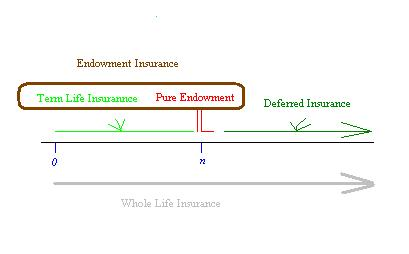
\includegraphics{Graphs/Graph_4_1_Deferred.jpg}
\end{center}
\caption{Different Insurance Contracts \label{FIGINSCONCLASS}}
\end{figure}
However, aside from these four types of policies, another type of insurance contract is displayed there which ``makes the picture complete" -- the so-called \textbf{$n$-year deferred insurance}. The corresponding present value random variable is of the following form:
$$
Z = \left\{\begin{array}{c l}
0 &,\, T_x \leq n \\
v^{T_x} &,\, T_x > n
\end{array}
\right. .
$$ 
Therefore, we have\
$$
{_{n|}\bar{A}_x} = E[Z] = \int_n^{\infty} v^t\,{_tp_x}\,{\mu_{x+t}}\,dt,
$$
and of course the rule of moments holds due to the level benefits, so that the second moment ${^2_{n|}\bar{A}_x}$ and, consequently, the variance can be determined in the ``usual" way. 

\section{Insurances Payable at the End of the Year of Death}
\label{SECPAYATENDOFYEAR}

So far, we have looked at insurances payable at the moment of death. Our approach was to define the present value random variable based on the future lifetime $T_x$. In general, in order to derive the expected present value -- the actuarial present value -- it was necessary to know or derive the distribution of $T_x$.

However, in practical applications, the only information available on the distribution of $T_x$ is given in the form of a discrete life table. Without an assumption on how the survival function evolves in between the discrete data given, i.e.\ an assumption about fractional ages, it is only possible to determine the distribution of a discretized version of the future lifetime: the curtate future lifetime $K_x$. Hence, in this section, we study insurances payable at the end of the year of death, and we rely on $K_x$ rather than $T_x$ to define the present value random variable. 

Let us, for example, consider a whole life insurance paying a benefit $b_{k+1}$ at $k+1$ upon death in year $[k,k+1)$, i.e.\ $T_x \in [k,k+1)$. Then, the present value of the payoff is :
%(see Figure \ref{FIGWHOLELIFEEND}).
$$
z_{k+1} = v_{k+1}\,b_{k+1}
$$
and the present value random variable is
\begin{eqnarray*}
Z &=& z_{k+1} \text{ if }k\leq T_x < k+1,\,k=0,1,2,...\\
&=& v_{k+1}\,b_{k+1} \text{ if }k = K_x,\,k=0,1,2,...\\
&=& v_{K_x+1}\,b_{K_x+1}.
\end{eqnarray*}
The (discrete!) distribution of $K_x$ is given by (cf.\ Sec.\ \ref{CURLIFTFORC})
$$
Pr\left(K_x=k\right) = {_{k|}q_x} = {_kp_x}\,{q_{x+k}}
$$
and, thus, for the actuarial present value we have in general
\begin{eqnarray*}
E[Z] &=& \sum_{k=0}^{\infty} v_{k+1}\,b_{k+1}\,Pr(K_x=k)
= \sum_{k=0}^{\infty} v_{k+1}\,b_{k+1}\,{_kp_x}\,{q_{x+k}},
\end{eqnarray*}
\begin{eqnarray*}
 E[Z^2] &=&  \sum_{k=0}^{\infty} \left(v_{k+1}\,b_{k+1}\right)^2\,Pr(K_x=k)
=  \sum_{k=0}^{\infty} v_{k+1}^2\,b_{k+1}^2\,\,{_kp_x}\,{q_{x+k}},
\end{eqnarray*}
and, clearly,
$$
Var[Z] = E[Z^2] - \left(E[Z]\right)^2.
$$

Based on these general formulas, we can now again consider level whole life, term-life, or deferred insurances. For a level whole life, we set $b_{k+1}=1,\,k=0,1,2,...$, and hence,\footnote{Again, we suppose a constant rate of interest $i$ in what follows.}
\begin{eqnarray*}
{A_x} &=& E[Z] = \sum_{k=0}^{\infty} \underbrace{v^{k+1}}_{= e^{-\delta\,(k+1)}}\,{_kp_x}\,{q_{x+k}},\\
{^2A_x} &=& E[Z^2] = \sum_{k=0}^{\infty} \underbrace{\left(v^{k+1}\right)^2}_{= e^{-2\,\delta\,(k+1)}}\,{_kp_x}\,{q_{x+k}},
\end{eqnarray*}
and the latter equation shows that, also here, the rule of moments is satisfied (for level benefits). In particular, we see that the same symbol is used for the actuarial present value without the bar -- i.e.\ the bar indicates that the insurance is payable at the moment of death rather than at the end of the year of death (without bar). Similarly to the previous section, we can now specify the other types of insurance in an analogous manner. For example, we have:
\begin{eqnarray*}
&\circ& {A_{\stackrel{1}{x}:\overline{n}|}} = \sum_{k=0}^{n-1} v^{k+1} {_kp_x}\,{q_{x+k}},\\
&\circ& {_{n|}A_x} = \sum_{k=n}^{\infty} v^{k+1} {_kp_x}\,{q_{x+k}},\\
&\circ& {A_{[x]+i}} = \sum_{k=0}^{\infty} v^{k+1} {_kp_{[x]+i}}\,{q_{[x]+i+k}}.\\
\end{eqnarray*}
The symbol for an $n$-year pure endowment policy, ${A_{x:\stackrel{1}{\overline{n}|}}}$, was introduced without a bar. The reason lies in the different payoff structure: A possible payment takes place only at time $n$ rather than at the time of death or at the end of the year of death. Hence, the formula remains valid:
\begin{eqnarray*}
Z &=& v^n,\,\text{ if } T_x>n 
= v^n,\,\text{ if } K_x \geq n\\
\Rightarrow {A_{x:\stackrel{1}{\overline{n}|}}} &=& v^n\,Pr\left(T_x>n\right) = v^n\,Pr\left(K_x\geq n\right)
= v^n\,{_np_x}.
\end{eqnarray*}
An $n$-year endowment policy payable at the end of the year of death thus has the actuarial present value:
$$
{A_{x:\overline{n}|}}={A_{\stackrel{1}{x}:\overline{n}|}} + {A_{x:\stackrel{1}{\overline{n}|}}}.
$$

\begin{homework}
\label{HW11}
\begin{enumerate}
\item Let $f_{20}(t) = \frac{1}{80}$, $0\leq t \leq 80$ (cf.\ first problem in Homework \ref{HW10}). Determine $\bar{A}_{\stackrel{1}{20}:\overline{10}|}$ and  $_{10|}\bar{A}_{20}$.
\item Assume mortality is described by $l_x = 100-x$ for $0\leq x \leq 100$ and that the force of interest is $\delta =0.05$.\footnote{This is Problem 4.6 in \cite{BOWERS}.}  
\begin{enumerate}
\item Calculate $\bar{A}_{\stackrel{1}{40}:\overline{25}|}$.
\item Determine the present actuarial value for a 25-year term insurance with benefit amount for death at time $t$, $b_t = e^{0.05\,t}$, for a person age 40 at policy issue.  
\end{enumerate} 
\item Assuming De Moivre's survival function with $\omega = 100$ and $i=0.10$, calculate\footnote{This is Problem 4.7 in \cite{BOWERS}.}  
\begin{enumerate}
\item Calculate $\bar{A}_{\stackrel{1}{30}:\overline{10}|}$.
\item The variance of the present value, at policy issue, of the benefit of the insurance in (a).
\end{enumerate} 
\item For a whole life insurance of $\$1,000$ on ($x$) with benefits payable at the moment of death, 
$$
\delta_t = \left\{\begin{array}{c l}
0.05 & ,\,0<t\leq10\\
0.06 & ,\,10<t
\end{array}\right.
$$
and
$$
\mu_{x+t} = \left\{\begin{array}{c l}
0.07 & ,\,0<t\leq10\\
0.08 & ,\,10<t
\end{array}\right.
$$
Calculate $E[Z]$.
\item The present value $Z$ of a so-called \textbf{$m$-year deferred $n$-year term insurance} on $(x)$ is 
$$
Z= \left\{\begin{array}{c l}
v^t & ,\,m< T_x \leq n+m\\
0 & ,\,\text{elsewhere}
\end{array}\right.
$$
and its actuarial present value is denoted by ${_{m|n}\bar{A}_x}$. What is the formula for this insurance? What about its variance? Can you think of any relationships to term or deferred policies?
\item Let $x=40$, $\delta=0.05$, and $\mu_{40+t}=\frac{1}{40}$. $Z$ denotes the present value random variable of a 5-year deferred insurance. Compute the actuarial present value and the variance of $Z$.
\item Let $x=30$, $\delta=0.06$, and $S_0(x)=1 - \frac{x}{100}$, $0\leq x \leq 100$. 
\begin{enumerate}
\item Find ${\bar{A}_{\stackrel{1}{30}:\overline{7}|}}$ and the variance of the corresponding present value random variable.
\item Find an approximate value $z$ such that the payoff for 1,000 independent insured lives with \$100,000 policies each will be lower than $z$ with a probability of 97.5\%.
\end{enumerate}
\item Let $\mu_{60+t} = \frac{1}{40}$, $t \geq 0$ and $\delta = 6\%$. 
\begin{enumerate}
\item Calculate the actuarial present value and the variance for a whole life policy on $(60)$ with benefits payable at the end of the year of death.
\item Calculate the actuarial present value and the variance for a 20-year endowment policy with benefits payable at the end of the year of death. 
\end{enumerate} 
\end{enumerate}
\end{homework}



\noindent \textbf{Solution} to Homework \ref{HW11}:
\footnotesize
\begin{enumerate} 
\item We have:
\begin{eqnarray*}
{\bar{A}_{\stackrel{1}{20}:\overline{10}|}} &=& \int_0^{10} v^t\, f_{20}(t)\,dt = \int_0^{10} e^{-t\,0.05} \frac{1}{80}\,dt\\
&=& \frac{1}{80 \cdot 0.05} \left(1 - e^{-10\cdot 0.05}\right) = 0.098367335,
\end{eqnarray*}
and for a 10-year deferred insurance we have 
\begin{eqnarray*}
{_{10|}\bar{A}_{20}} &=& \int_{10}^{\infty} v^t\,f_{20}(t)\,dt = \int_{10}^{80} e^{-t\,0.05} \frac{1}{80}\,dt\\
&=& \frac{1}{80 \cdot 0.05} \left(e^{-0.05\cdot 10} - e^{-0.05\cdot 80}\right) = .147053755 \\
&=& \bar{A}_{20} - {\bar{A}_{\stackrel{1}{20}:\overline{10}|}},
\end{eqnarray*}
which does not seem surprising regarding Figure \ref{FIGINSCONCLASS}. However, again this relationship does \underline{not} hold for the variances (but of course the rule of moments holds)!
\item
(a):
\begin{eqnarray*}
l_x &=& 100 -x \text{ (DeMoivre)},\,\,\mu_x = \frac{-S_0'(x)}{S_0(x)} = \frac{-l'_x}{l_x} = \frac{1}{l_x}, \\
{\bar{A}_{\stackrel{1}{40}: \overline{25}|}} &=&
\int_0^{25} e^{-0.05\,t}\,\frac{l_{40+t}}{l_{40}}\, \underbrace{\mu_{40+t}}_{= \frac{1}{l_{40+t}}}\,dt,\\
&=& \frac{1}{l_{40}} \int_0^{25} e^{-0.05\,t}\,dt = \frac{1}{60\cdot 0.05} (1- e^{-0.05 \cdot 25}) =0.23783173.
\end{eqnarray*}
(b):
\begin{eqnarray*}
E[Z] &=& \int_0^{25} e^{-0.05\,t}\,e^{0.05\,t}\,\frac{l_{40+t}}{l_{40}}\, \underbrace{\mu_{40+t}}_{= \frac{1}{l_{40+t}}}\,dt \\
&=& \frac{1}{l_{40}} \int_0^{25}\,dt = \frac{25}{60} = \frac{5}{12}.
\end{eqnarray*}
\item (a):  
$$
i = 0.1 \Rightarrow  \delta = \log(1.1) = 0.09531.
$$
\begin{eqnarray*}
{\bar{A}_{\stackrel{1}{30}:\overline{10}|}} &=& \int_0^{10} e^{-0.09531\,t}\,\frac{S_0(x+t)}{S_0(x)}\,\frac{-S_0'(x+t)}{S_0(x+t)}\,dt\\
&=& \int_0^{10} \,e^{-0.0531\,t}\,\frac{1}{100-30}\,dt = \frac{1}{70 \cdot 0.09531} \left(1 - e^{-0.9531}\right)\\
&=&0.0920988.
\end{eqnarray*}
(b): 
\begin{eqnarray*}
{^2\bar{A}_{\stackrel{1}{30}:\overline{10}|}} &=& \int_0^{10} e^{-2\,0.09531\,t}\,\frac{S_0(x+t)}{S_0(x)}\,\frac{-S_0'(x+t)}{S_0(x+t)}\,dt\\
&=& \int_0^{10} \,e^{-2\,0.09531\,t}\,\frac{1}{100-30}\,dt = \frac{1}{70 \cdot 2 \cdot 0.09531} \left(1 - e^{-10 \cdot 2 \cdot 0.09531}\right)\\
&=&0.66380\\
\Rightarrow Var[Z] &=& {^2\bar{A}_{\stackrel{1}{30}:\overline{10}|}}  - \left({\bar{A}_{\stackrel{1}{30}:\overline{10}|}} \right)^2 = 0.0553.
\end{eqnarray*} 
\item For the discount function and the survival probability, we have:
\begin{eqnarray*}
v_t &=& e^{-\int_0^t \delta_s\,ds} = \left\{
\begin{array}{cl}
e^{-0.05\,t},&0\leq t < 10\\
e^{-0.05\,10}\,e^{-0.06\,(t-10)},& t\geq 10
\end{array}
\right. \\
{_tp_x} &=& e^{-\int_0^t \mu_{x+s}\,ds} = \left\{
\begin{array}{cl}
e^{-0.07\,t},&0\leq t < 10\\
e^{-0.07\,10}\,e^{-0.08\,(t-10)},& t\geq 10
\end{array}
\right.\\
\Rightarrow {_tp_x}\,\mu_{x+t} &=& e^{-\int_0^t \mu_{x+s}\,ds} \mu_{x+s} = \left\{
\begin{array}{cl}
0.07\,e^{-0.07\,t},&0\leq t < 10\\
0.08\,e^{-0.07\,10}\,e^{-0.08\,(t-10)},& t\geq 10
\end{array}
\right.\\
\Rightarrow
E[Z]/1000 &=& \int_0^\infty b_t\,v_t\,{_tp_x}\,\mu_{x+t}\,dt\\
&=& \int_0^{10} e^{-0.05\,t}\,e^{-0.07\,t}\,0.07\,dt \\&&
+ \int_{10}^{\infty} e^{-0.05\,10} e^{-0.06\,(t-10)}\,e^{-0.07\,10} \,e^{-0.08\,(t-10)}\,0.08\,dt\\
&=& 0.07\,\frac{1 - e^{-1.2}}{0.12} + 0.08\,e^{-1.2}\, \int_{10}^\infty e^{-0.14 \,(t-10)} \,dt \\
&=& .40763671 + .172110978 = .519747688
\end{eqnarray*}
\begin{eqnarray*}
\Rightarrow E[Z] &=& 519.747688.
\end{eqnarray*}
\item \begin{eqnarray*}
{_{m|n}\bar{A}_x} &=& \int_m^{m+n} v^t\,{_tp_x}\,\mu_{x+t}\,dt\\
{\bar{A}_x} &=& {\bar{A}_{\stackrel{1}{x}:\overline{m}|}}  + {_{m|n}\bar{A}_x} +  {_{m+n|}\bar{A}_x}  
\end{eqnarray*}
The variance can be calculated as usual via the rule of moments.
\item
\begin{eqnarray*}
{_tp_x} &=& e^{-\int_0^t \mu_{x+s}\,ds} = e^{-0.025\,t}\\
\Rightarrow f_{T} (t) &=& {_tp_x}\,\mu_{x+t} = 0.025\,e^{-0.025\,t}\\
\Rightarrow {_{5|}\bar{A}_{40}} &=& \int_5^\infty v^t \, f_T(t)\,dt\\
&=& 0.025 \int_5^\infty e^{-0.075\,t}\,dt = 0.229096426\\
 {^2_{5|}\bar{A}_{40}} &=& \int_5^\infty v^{2t} \, f_T(t)\,dt\\
&=& 0.025 \int_5^\infty e^{-0.125\,t}\,dt = 0.107052286\\
\Rightarrow Var(Z) &=&  {^2_{5|}\bar{A}_{40}} - ({_{5|}\bar{A}_{40}})^2 = .054567113.
\end{eqnarray*}

\item
\begin{eqnarray*}
\mu_{x+t} &=& \frac{1}{100 - (x+t)}\\
\Rightarrow {\bar{A}_{\stackrel{1}{30}:\overline{7}|}} &=& \int_0^7 v^t \, {_tp_{30}}\,\mu_{30+t}\,dt\\
&=& \int_0^7 v^t \frac{S_0(30+t)}{S_0(30)} \frac{1}{100\,S_0(30+t)}\,dt\\
&=& \frac{1}{100\,S_0(30)} \int_0^7 e^{-0.06\,t}\,dt = 0.081655519\\
\Rightarrow {^2\bar{A}_{\stackrel{1}{30}:\overline{7}|}} &=& \int_0^7 v^{2t} \, {_tp_{30}}\,\mu_{30+t}\,dt\\
&=& \int_0^7 v^{2t} \frac{S_0(30+t)}{S_0(30)} \frac{1}{100\,S_0(30+t)}\,dt\\
&=& \frac{1}{100\,S_0(30)} \int_0^7 e^{-0.12\,t}\,dt = 0.067653509\\
Var(z) &=& 0.067653509 - 0.081655519^2 = .06098589\\
\sigma &=& 0.246953205.
\end{eqnarray*}

For 1,000 lives with \$100,000 policies each:
\begin{eqnarray*}
\text{Mean }\mu &=& n\cdot d \cdot {\bar{A}_{\stackrel{1}{30}:\overline{7}|}} = 8,165,551.90\\
\text{Variance } \sigma^2 &=& n\cdot d^2 \cdot Var(z) = 6.0985885\cdot 10^{11}\\
\Rightarrow \sigma &=& 780,934.6003\\
\stackrel{\text{CLT}}{\Rightarrow} \xi^{0.9} &=& \mu + 1.96\cdot \sigma = \$ 9,696,183.72
\end{eqnarray*}
is the approximative 97.5th percentile by the normal approximation (1.96 is the 97.5th percentile of the Normal distribution).
\item For the actuarial present value and the variance for a 20-year endowment policy, we have:
\begin{eqnarray*}
v &=& e^{-\delta} = .941764534\\
{_tp_x} &=& e^{-\frac{t}{40}}\\
q_{x+t} &=& 1 - p_{x+t} = 1 - e^{-\frac{1}{40}} = .02469088\\
\Rightarrow {A_{60}} &=& \sum_{k=0}^{\infty} v^{k+1}\,e^{-\frac{k}{40}}\,0.02469088 = 0.02469088\left[v\sum_{k=0}^{\infty} \left(v\,e^{-\frac{1}{40}}\right)^k\right] \\
&=& 0.02469088\, v\,\frac{1 }{1 -  \left(v\,e^{-\frac{1}{40}}\right)}  = 0.285355836 \\
\text{and } {A_{60:\overline{20}|}} &=& \sum_{k=0}^{19} v^{k+1}\,e^{-\frac{k}{40}}\,0.02469088 + v^{20}e^{-\frac{20}{40}}\\
&=& 0.02469088\left[v\sum_{k=0}^{19} \left(v\,e^{-\frac{1}{40}}\right)^k\right] + 0.182683524\\
&=& 0.02469088\, v\,\frac{1 -  \left(v\,e^{-\frac{1}{40}}\right)^{20}}{1 -  \left(v\,e^{-\frac{1}{40}}\right)} +
 0.182683524 = 0.415902067.
 \end{eqnarray*}
 Similarly:
 \begin{eqnarray*}
 Var(Z^{\text{whole}})&=&   {^2A_{60}} - \left( A_{60} \right)^2\\
 &=&  0.02469088\, \tilde{v}\,\frac{1 }{1 -  \left(\tilde{v}\,e^{-\frac{1}{40}}\right)}  - (0.285355836)^2\\
 &=& 0.080812514\\ 
 \text{and }Var(Z^{\text{end}})&=&   {^2A_{60:\overline{20}|}} - \left( {A_{60:\overline{20}|}} \right)^2\\
 &=&   0.02469088\, \tilde{v}\,\frac{1 -  \left(\tilde{v}\,e^{-\frac{1}{40}}\right)^{20}}{1 -  \left(\tilde{v}\,e^{-\frac{1}{40}}\right)}  + \tilde{v}^{20}e^{-\frac{20}{40}} - (0.415902067)^2\\
 &=& 0.035341403.
\end{eqnarray*}

\end{enumerate}
\normalsize



Similar to the curtate expectation of lifetime, we can now derive recursion relationships, which present important tools in practical applications:
\begin{eqnarray}
A_x &=&  \sum_{k=0}^{\infty} v^{k+1} {_kp_x}\,{q_{x+k}} = v\,{_0p_x}\,{q_x} +  \sum_{k=1}^{\infty} v^{k+1} {_kp_x}\,{q_{x+k}}\nonumber \\
&=& v\,{q_x} +  v\,p_x\,\sum_{k=1}^{\infty} v^{k-1+1} {_{k-1}p_{x+1}}\,{q_{x+1+(k-1)}} \nonumber\\
&\stackrel{l=k-1}{=} & v\,{q_x} +  v\,p_x\,\sum_{l=0}^{\infty} v^{l+1} {_{l}p_{x+1}}\,{q_{x+1+l}} \nonumber\\
&=& v\,{q_x} +  v\,p_x\,{A_{x+1}} = v\cdot {q_x} + v\cdot p_x\cdot {A_{x+1}}. \label{EQRECRELFORAX}
\end{eqnarray}
Analogously, recursion relationships for the other types of insurance policies can be determined:
\begin{eqnarray*}
 {A_{\stackrel{1}{x}:\overline{n}|}}  &=& v\cdot {q_x} + v\cdot p_x\cdot {A_{\stackrel{1}{x+1}:\overline{n-1}|}},\\
 {A_{x:\stackrel{1}{\overline{n}|}}} &=& v\cdot p_x \cdot  {A_{x+1:\stackrel{1}{\overline{n-1}|}}}, \\
 {A_{x:\overline{n}|}} &=& v\cdot q_x + v\cdot p_x \cdot {A_{x+1:\overline{n-1}|}},\\
 {_{n|}A_x}  &=& v\cdot p_x \cdot {_{n-1|}A_{x+1}},\\
 A_{[x]+i} &=& v\cdot {q_{[x]+i}} + v\cdot p_{[x]+i}\cdot {A_{[x]+i+1}}.
\end{eqnarray*}

Based on the recursion relationship for $A_x$, we can now ``fill up" an entire life table. Given the ``fundamentals" or ``basis for actuarial calculation" $i$ and $q_x$, $x=0,1,2,...$, with $A_{\omega} = v\cdot q_{\omega} = v$, we can now derive $A_{\omega-1},\,A_{\omega-2},\,...,\, A_2,\,A_1,\,A_0$ based on (\ref{EQRECRELFORAX}).  

\noindent \textbf{Example:} 
\begin{eqnarray*}
A_{36} &=& .1347002 \\
i &=& 0.06 \, \Rightarrow v = \frac{1}{1.06} = .943396226\\
q_{35} &=& 0.0020136 \, \Rightarrow p_{35} = .9979864 \\
\Rightarrow A_{35} &=& v\,q_{35} + v\,p_{35}\,A_{36}\\
&=&.943396226\cdot 0.0020136 + .943396226\cdot .9979864\cdot .1347002\\
&=& .1287194.
\end{eqnarray*}
Since the same recursion holds for the second moment by the rule of moments, the same can be done for $^2A_{36}$ so that the ``ingredients" for determining the actuarial present value as well as the variance are readily available. 

Similarly, we could ``fill up" columns for other insurances, but in fact this is not necessary since the presented information already suffices to determine the expected present values and the variances. For a pure endowment policy, we have
$$
{A_{x:\stackrel{1}{\overline{n}|}}} = v^n \, {_np_x} = \left(\frac{1}{1+i}\right)^n \frac{l_{x+n}}{l_x}
$$
which can be readily derived if the basis for actuarial calculation are available. Moreover, we have:
\begin{eqnarray*}
A_x &=& \sum_{k=0}^\infty v^{k+1}\,{_kp_x}\,q_{x+k}\\
&=& \underbrace{\sum_{k=0}^{n-1}v^{k+1}\,{_kp_x}\,q_{x+k}}_{={A_{\stackrel{1}{x}:\overline{n}|}}} \,+\, \sum_{k=n}^\infty v^{k+1}\,{_kp_x}\,q_{x+k} \\
&=& {A_{\stackrel{1}{x}:\overline{n}|}} + \underbrace{{v^n}\,{_np_x}}_{= A_{x:\stackrel{1}{\overline{n}|}}}\,\sum_{k=n}^\infty v^{k-n+1}\,{_{k-n}p_{x+n}}\,q_{x+n+k-n} 
\stackrel{l=k-n}{=} {A_{\stackrel{1}{x}:\overline{n}|}} + {A_{x:\stackrel{1}{\overline{n}|}}}
\underbrace{\sum_{l=0}^\infty v^{l+1}\,{_lp_{x+n}}\,q_{x+n+l}}_{=A_{x+n}}
\end{eqnarray*}
\begin{eqnarray*}
\Rightarrow  {A_{\stackrel{1}{x}:\overline{n}|}} &=& A_x\,-\, {A_{x:\stackrel{1}{\overline{n}|}}}\,
A_{x+n}\\
\Rightarrow
{A_{x:\overline{n}|}} &=& {A_{\stackrel{1}{x}:\overline{n}|}} + {A_{x:\stackrel{1}{\overline{n}|}}} = A_x + (1-A_{x+n})\cdot {A_{x:\stackrel{1}{\overline{n}|}}} \\
\text{and }{_{n|}A_x} &=& A_x - {A_{\stackrel{1}{x}:\overline{n}|}} = {A_{x:\stackrel{1}{\overline{n}|}}} \cdot A_{x+n}.
\end{eqnarray*}
Thus, given a life table, $i$, and the additional $A_x$ column, we can derive the actuarial present values for term-life, deferred life, and endowment insurances. Again, by the rule of moments, the same steps can be taken out for the second moment,\footnote{Note that ${^2A_{x:\stackrel{1}{\overline{n}|}}} = v^{2n} \, {_np_x}$.} so that we can also derive the second moments and thus the variances for these insurances when given the $^2A_x$-column.

In the foregoing section, we considered benefits payable at the moment of death. In particular, we derived the actuarial present values and variances of several types of policies under a specified mortality law, such as the De Moivre mortality law. Since in actuarial practice, life tables rather than analytic mortality laws are employed, it is of interest how to derive these values from life tables. However, as payments can occur at any point in time, i.e.\ the time of death can take every value greater or equal to zero, but information about the survival function is only available discretely (life table), assumptions about an interpolation schemes or, in other words, assumptions about fractional ages need to be made.

Let us for example consider a whole life insurance with benefits payable at the moment of death:
\begin{eqnarray*}
{\bar{A}_x} &=& \int_0^\infty v^t\,{_tp_x}\,{\mu_{x+t}}\,dt\\
&=& \int_0^1 v^t\,{_tp_x}\,{\mu_{x+t}}\,dt + \int_1^\infty v^t\,{_tp_x}\,{\mu_{x+t}}\,dt\\
&=& \int_0^1 v^t\,{_tp_x}\,{\mu_{x+t}}\,dt + v\,{p_x}\int_1^\infty v^{t-1}\,{_{t-1}p_{x+1}}\,{\mu_{x+1+t-1}}\,dt\\
&\stackrel{u=t-1}{=}& \int_0^1 v^t\,{_tp_x}\,{\mu_{x+t}}\,dt + v\,{p_x}\underbrace{\int_0^\infty v^{u}\,{_{u}p_{x+1}}\,{\mu_{x+1+u}}\,dt}_{={\bar{A}_{x+1}}}.
\end{eqnarray*}
Under the assumption of a uniform distribution of deaths over the year, we obtain
$$
{_tp_x}\,{\mu_{x+t}} = (1 - t\cdot q_x)\cdot \frac{q_x}{1-t\,q_x} = q_x,\;0\leq t < 1,
$$
and therefore,
\begin{eqnarray*}
{\bar{A}_x} &=& q_x\, \int_0^1 v^t\,dt + v\,{p_x}\,{\bar{A}_{x+1}} = q_x\,\frac{1}{\log\{v\}}\,(v-1) + v\,{p_x}\,{\bar{A}_{x+1}}\\
&=& \frac{i}{\delta} v \, q_x +  v\,{p_x}\,{\bar{A}_{x+1}}.
\end{eqnarray*}
However, from this we obtain:
\begin{eqnarray*}
{\bar{A}_x} &=& \frac{i}{\delta} v \, q_x +  v\,{p_x}\,{\bar{A}_{x+1}}
   = \frac{i}{\delta} v \, q_x +  v\,{p_x}\,\left({\frac{i}{\delta} v \, q_{x+1} +  v\,{p_{x+1}}\,{\bar{A}_{x+2}}}\right)\\
   &=& \frac{i}{\delta} v \, q_x +  v\,{p_x}\,\left(\frac{i}{\delta} v \, q_{x+1} +  v\,{p_{x+1}}\,\left({\frac{i}{\delta} v \, q_{x+2} +  v\,{p_{x+2}}\,{\bar{A}_{x+3}}}\right)\right)\\
&=&...\\
&=&\frac{i}{\delta}\left(vq_x + v^2\,{p_x}\,{q_{x+1}} + v^3\,{_2p_x}\,{q_{x+2}} + ...\right)\\
&=& \frac{i}{\delta} \sum_{k=0}^\infty v^{k+1}\,{_kp_x}\,q_{x+k} \\
&=& \frac{i}{\delta} \,A_x.
\end{eqnarray*}
Clearly, the rule of moments holds again in this case, but clearly the interest rate $i$ in the latter formula needs to be adjusted. Moreover, a similar argument works for ${\bar{A}}_{\stackrel{1}{x}:\overline{n}|}$. Here, we have:
$$
{\bar{A}}_{\stackrel{1}{x}:\overline{n}|} = \frac{i}{\delta} \, {A}_{\stackrel{1}{x}:\overline{n}|}.
$$ 

\begin{homework}
\label{HW12}
\begin{enumerate}
\item If $A_x = 0.25$, $A_{x+20} = 0.40$, and $A_{x:\overline{20}|}=0.55$, calculate (a) $A_{x:\stackrel{1}{\overline{20}|}}$ and (b) $A_{\stackrel{1}{x}:\overline{20}|}$.\footnote{This is Problem 4.16 in \cite{BOWERS}.}  
\item For a special 3-year term insurance on $(x)$ you are given: 
\begin{enumerate}
\item Z is the present-value random variable for this insurance.
\item $q_{x+k} = 0.02(k+1),$ $k=0,1,2$.
\item The following benefits are payable at the end of the year of death:
\begin{center}
\begin{tabular}{|c|c|}
\hline
$k$ & $b_{k+1}$ \\
\hline
0 & 300 \\
1 & 350 \\
2 & 400 \\
\hline
\end{tabular}
\end{center}
\item $i=0.06$.
\end{enumerate}
Calculate $Var(z)$.
\item The actuarial present value of an \textbf{$m$-year deferred $n$-year term insurance} payable at the end of the year of death is denoted by  ${_{m|n}A_x}$. What is the formula for this insurance? What about its variance? 
\item \label{HW12a} From the SOA illustrative life table, derive
\begin{enumerate}
\item ${A_{35:\stackrel{1}{\overline{30}|}}}$,
${A_{\stackrel{1}{35}:\overline{30}|}}$,
${A_{35:\overline{30}|}}$, 
${_{30|}A_{35}}$ as well as the variances for these insurances.
\item ${\bar{A}_{35}}$,
${\bar{A}_{\stackrel{1}{35}:\overline{30}|}}$, 
${\bar{A}_{35:\overline{30}|}}$, 
${_{30|}\bar{A}_{35}}$ as well as the variances for these insurances under the assumption of a uniform distribution of deaths over each year of age.
\end{enumerate}
\item \label{MTHLYINS} Consider a timescale measured in intervals of length $\frac{1}{m}$ where the unit is a year. Let a whole life insurance for a unit amount be payable at the end of the $m$-thly interval in which death occurs. Let $k$ be the number of complete insurance years lived prior to death and let $j$ be the number of complete $m$-ths of a year lived in the year of death.\footnote{This is Problem 4.19 in \cite{BOWERS}.}  
\begin{enumerate}
\item What is the present-value random variable for this insurance?
\item Set up a recursion relationship for the actuarial present value, $A_x^{(m)}$, for this insurance.
\item Show algebraically that, under the assumption of a uniform distribution of deaths over the insurance year of age,
$$
A_x^{(m)} = \frac{i}{i^{(m)}}\,A_x.
$$
\end{enumerate}
\item Show, under the assumption of a constant force of mortality between integer-valued ages, that
$$
\bar{A}_x = \sum_{k=0}^{\infty} v^{k+1}\,{_kp_x}\,\mu_{x+k}\,\frac{i+q_{x+k}}{\delta + \mu_{x+k}},
$$
where $\mu_{x+k} = - \log\{p_{x+k}\}$.\footnote{This is Problem 4.20 in \cite{BOWERS}.} 
\item Using Part \ref{HW12a} and Part \ref{MTHLYINS}, derive ${A^{(12)}_{35}}$,
${A^{(12)}_{\stackrel{1}{35}:\overline{30}|}}$, 
${A^{(12)}_{35:\overline{30}|}}$ as well as the variances for these insurances under the assumption of a uniform distribution of deaths over each year of age.
\end{enumerate}
\end{homework}
%\newpage
\noindent \textbf{Solution} to Homework \ref{HW12}:
\footnotesize
\begin{enumerate}
\item We have
\begin{eqnarray*}
A_x &=&  \sum_{k=0}^{\infty} v^{k+1} {_kp_x}\,{q_{x+k}} \\
&=&  \sum_{k=0}^{20-1} v^{k+1} {_kp_x}\,{q_{x+k}} +  \sum_{k=20}^{\infty} v^{k+1} {_kp_x}\,{q_{x+k}} \\
&=&  {A_{\stackrel{1}{x}:\overline{20}|}} + v^{20}\,{_{20}p_x}  \sum_{k=20}^{\infty} v^{k-20+1} {_{k-20}p_{x+20}}\,{q_{x+20+k-20}}\\
&\stackrel{l=k-20}{=} &  {A_{\stackrel{1}{x}:\overline{20}|}} + v^{20}\,{_{20}p_x}  \sum_{l=0}^{\infty} v^{l+1} {_{l}p_{x+20}}\,{q_{x+20+l}}\\
&=&   {A_{\stackrel{1}{x}:\overline{20}|}} + {A_{x:\stackrel{1}{\overline{20}|}}}  \,A_{x+20}\\
 {A_{x:\overline{n}|}} &=& {A_{\stackrel{1}{x}:\overline{20}|}}  +  {A_{x:\stackrel{1}{\overline{20}|}}}  
 \end{eqnarray*}
\begin{eqnarray*}
 \Rightarrow {A_{\stackrel{1}{x}:\overline{20}|}} &=& {A_{x:\overline{20}|}}  - {A_{x:\stackrel{1}{\overline{20}|}}} \\
\Rightarrow 
A_x &=& {A_{x:\overline{20}|}}  - {A_{x:\stackrel{1}{\overline{20}|}}} + {A_{x:\stackrel{1}{\overline{20}|}}  }\,A_{x+20}\\
&=& {A_{x:\overline{20}|}}  + {A_{x:\stackrel{1}{\overline{20}|}}} \left( A_{x+20} - 1\right)\\
&=& 0.55 + {A_{x:\stackrel{1}{\overline{20}|}} }\left(0.4 - 1\right)\\
\Rightarrow
{A_{x:\stackrel{1}{\overline{20}|}}} &=& \frac{0.25-0.55}{-0.6} = 0.5\\
  {A_{\stackrel{1}{x}:\overline{20}|}} &=&  {A_{x:\overline{20}|}} -  {A_{x:\stackrel{1}{\overline{20}|}}} =
  0.55 - 0.5 = 0.05.
  \end{eqnarray*}
\item
 \begin{eqnarray*}
 E[Z] &=& \sum_{k=0}^2 {_kp_x} \, {q_{x+k}}\,v^{k+1} \, b_{k+1}\\
 &=& 0.02 \cdot v \cdot 300 + 0.98\cdot 0.04 \cdot v^2 \cdot 350 + 0.98\cdot 0.96 \cdot 0.06 \cdot v^3 \cdot 400\\
 &=& 36.82906023
 \end{eqnarray*}
 \begin{eqnarray*}
 E[Z^2] &=& \sum_{k=0}^2 {_kp_x} \, {q_{x+k}}\,v^{2k+2} \, b_{k+1}^2\\
 &=& 0.02 \cdot v^2 \cdot 300^2 + 0.98\cdot 0.04 \cdot v^4 \cdot 350^2 + 0.98\cdot 0.96 \cdot 0.06 \cdot v^6 \cdot 400^2\\
 &=& 11,772.60538\\
 \Rightarrow Var[Z] &=& E[Z^2] - \left(E[Z]\right)^2 = 10,493.85.
 \end{eqnarray*}
 \item
 $$%\begin{eqnarray*}
 {_{m|n}A_x} = \sum_{k=m}^{m+n-1} v^{k+1}\,{_kp_x}\,{q_{x+k}}.
 $$%\end{eqnarray*}   
Variance via the rule of moments:
$$
Var[Z] = {^2_{m|n}A_x} - \left({_{m|n}A_x}\right)^2.
$$
\item
\begin{enumerate}
\item 
\begin{itemize}
 \item
 \begin{eqnarray*}
 {A_{35:\stackrel{1}{\overline{30}|}}} &=& {_{30}p_{35}}\,v^{30} = \frac{l_{65}}{l_{35}}\,(1+i)^{-30}\\
 &=& \frac{75,339.63}{94,206.55}\frac{1}{1.06^{30}} = .13924077,\\
 {^2A_{35:\stackrel{1}{\overline{30}|}}} &=& {_{30}p_{35}}\,(\underbrace{\tilde{v}}_{=(e^{-2\,\delta})=v^2})^{30} = \frac{l_{65}}{l_{35}}\,(1+i)^{-60}\\
 &=& \frac{75,339.63}{94,206.55}\frac{1}{1.06^{60}} = .02424323,\\
 Var(Z) &=& .02424323 - .13924077^2 = .00485524.
 \end{eqnarray*}
 \item
 \begin{eqnarray*}
 {A_{\stackrel{1}{35}:\overline{30}|}} &=& {A_{35}} -  {A_{35:\stackrel{1}{\overline{30}|}}} \,{A_{65}}\\
 &=& .1287194 - .13924077\cdot .4397965 = .0674818,\\
 {^2A_{\stackrel{1}{35}:\overline{30}|}} &=& {^2A_{35}} -  {^2A_{35:\stackrel{1}{\overline{30}|}}} \,{^2A_{65}}\\
 &=& .0348843 - .02424323\cdot .2360299 = .02916217,\\
 Var(Z) &=& .02916217 - .0674818^2 = .02460838.
 \end{eqnarray*}
 \item
 \begin{eqnarray*}
 {A_{35:\overline{30}|}} &=&  {A_{35:\stackrel{1}{\overline{30}|}}}  +  {A_{\stackrel{1}{35}:\overline{30}|}}\\
 &=& .13924077 + .0674818 = .20672257,\\
 {^2A_{35:\overline{30}|}} &=&  {^2A_{35:\stackrel{1}{\overline{30}|}}}  +  {^2A_{\stackrel{1}{35}:\overline{30}|}}\\
 &=& .02424323 + .02916217 = .0534054,\\
 Var(Z) &=& .0534054 -  .20672257^2 = .01067118.
 \end{eqnarray*}
 Careful! This is not the sum of the respective variances!
 \item
 \begin{eqnarray*}
 {_{30|}A_{35}} &=& {A_{35}} -  {A_{\stackrel{1}{35}:\overline{30}|}} \\
 &=& .1287194 - .0674818 = .0612376,\\
 {^2_{30|}A_{35}} &=& {^2A_{35}} -  {^2A_{\stackrel{1}{35}:\overline{30}|}} \\
 &=& .0348843 - .02916217 = .00572213,\\
 Var(Z) &=& .00572213 - .0612376^2 = .00197208.
 \end{eqnarray*}
\end{itemize}
\item We have $i = 0.06 \Rightarrow \delta = \log\{1+i\} = 0.058269$ and, thus, for the second moments by the rule of moments $\delta^* = 2\cdot \delta = 0.116358 \Rightarrow i^* = e^{\delta^*} = 0.1236$. 
 \begin{eqnarray*}
 {\bar{A}_{35}} &=& \frac{i}{\delta} {A_{35}} = \frac{0.06}{0.058269} 0.1287194 = 0.132543,\\
 {^2\bar{A}_{35}} &=& \frac{i^*}{\delta^*}\, {^2A_{35}} = \frac{0.1236}{0.1164} \,0.0348843 = 0.036998,\\
 \Rightarrow Var[Z] &=&  {^2\bar{A}_{35}} - \left({\bar{A}_{35}}\right)^2 = 0.019431.\\
 {\bar{A}_{\stackrel{1}{35}:\overline{30}|}} &=&\frac{i}{\delta}    {A_{\stackrel{1}{35}:\overline{30}|}} 
= \frac{0.06}{0.058269} 0.0674818 = 0.069487,\\
{^2\bar{A}_{\stackrel{1}{35}:\overline{30}|}} &=&\frac{i^*}{\delta^*} \, {^2A_{\stackrel{1}{35}:\overline{30}|}} 
= \frac{0.1236}{0.1164} \,0.02916217 = 0.030929,\\
\Rightarrow Var[Z] &=&  {^2\bar{A}_{\stackrel{1}{35}:\overline{30}|}} - \left({\bar{A}_{\stackrel{1}{35}:\overline{30}|}} \right)^2 = 0.026101.\\
 {\bar{A}_{35:\overline{30}|}} &=&  {A_{35:\stackrel{1}{\overline{30}|}}}  +  {\bar{A}_{\stackrel{1}{35}:\overline{30}|}} =  0.13924077 + 0.069487 = 0.2087277,\\
 {^2\bar{A}_{35:\overline{30}|}} &=&  {^2A_{35:\stackrel{1}{\overline{30}|}}}  +  {^2\bar{A}_{\stackrel{1}{35}:\overline{30}|}} = 0.02424323 + 0.030929 = 0.05517223,\\
 \Rightarrow Var[Z] &=&  {^2\bar{A}_{35:\overline{30}|}}  - \left({\bar{A}_{35:\overline{30}|}} \right)^2
 = 0.011604977.\\
 {_{30|}\bar{A}_{35}} &=& {\bar{A}_{35}} -  {\bar{A}_{\stackrel{1}{35}:\overline{30}|}}  = 0.063056,\\
 {^2_{30|}\bar{A}_{35}} &=& {^2\bar{A}_{35}} -  {^2\bar{A}_{\stackrel{1}{35}:\overline{30}|}} = 0.006069, \\
 \Rightarrow Var[Z] &=&  {^2_{30|}\bar{A}_{35}}  - \left( {_{30|}\bar{A}_{35}} \right)^2 = 0.002092941.
\end{eqnarray*}
\end{enumerate}
\item For $\frac{l}{m} \leq T < \frac{l+1}{m}$, we have a present value of $v^{\frac{l+1}{m}}$. Therefore,
\begin{eqnarray*}
{A_x^{(m)}} &=& E[Z] = \sum_{l=0}^{\infty} v^{\frac{l+1}{m}} Pr\left(\frac{l}{m} \leq T < \frac{l+1}{m}\right) \\
&=& \sum_{l=0}^{\infty}  v^{\frac{l+1}{m}} \,{_{\frac{l}{m}}p_x}\,{_{\frac{1}{m}}q_{x+\frac{l}{m}}}\\
&=& \sum_{k=0}^{\infty} \sum_{j=0}^{m-1} v^{k+\frac{j+1}{m}} \,{_{k+\frac{j}{m}}p_x}\,{_{\frac{1}{m}}q_{x+k+\frac{j}{m}}}
 \end{eqnarray*}
 \begin{eqnarray*}
&=&\sum_{k=0}^{\infty}  v^{k} \,{_{k}p_x}\sum_{j=0}^{m-1} v^{\frac{j+1}{m}} \,{_{\frac{j}{m}}p_{x+k}}\,{_{\frac{1}{m}}q_{x+k+\frac{j}{m}}}\\
&\stackrel{\text{Unif.\ Ass.}}{=}&  \sum_{k=0}^{\infty}  v^{k} \,{_{k}p_x}\sum_{j=0}^{m-1} v^{\frac{j+1}{m}} \,\underbrace{{_{\frac{j}{m}}p_{x+k}}\,{_{\frac{1}{m}}q_{x+k+\frac{j}{m}}}}_{={_{\left.\frac{j}{m}\right|\frac{1}{m}}q_{x+k}}= \frac{1}{m}\cdot q_{x+k}} 
%\end{eqnarray*}
%\begin{eqnarray*}
%&=&  
= \sum_{k=0}^{\infty}  v^{k+1} \,{_{k}p_x}\,{q_{x+k}}\sum_{j=0}^{m-1} \frac{v^{\frac{j+1}{m}-1}}{m}.
\end{eqnarray*} 
Now, 
\begin{eqnarray*}
&&\sum_{j=0}^{m-1} \frac{v^{\frac{j+1}{m}-1}}{m}
= \frac{v^{\frac{1}{m}}}{m \cdot v} \sum_{j=0}^{m-1} \left(v^{\frac{1}{m}}\right)^j\\
&=& \frac{v^{\frac{1}{m}}}{m \cdot v} \frac{1 - \left(v^{\frac{1}{m}}\right)^{m}}{1 - v^{\frac{1}{m}}}
= \frac{i}{m\left((1+i)^{\frac{1}{m}} - 1\right)} = \frac{i}{i^{(m)}}.
\end{eqnarray*}
Hence,
\begin{eqnarray*}
{A_x^{(m)}} &=&  \sum_{k=0}^{\infty}  v^{k+1} \,{_{k}p_x}\,{q_{x+k}}\sum_{j=0}^{m-1} \frac{v^{\frac{j+1}{m}-1}}{m}\\
&=& \sum_{k=0}^{\infty}  v^{k+1} \,{_{k}p_x}\,{q_{x+k}} \frac{i}{i^{(m)}}
= \frac{i}{i^{(m)}} \,{A_x}.
\end{eqnarray*}

\noindent \textbf{Remark}: We have
\begin{eqnarray*}
{A_x^{(m)}} &=& \frac{i}{i^{(m)}} {A_x} \\
&=& \frac{i}{m\left(e^{\frac{\delta}{m}} - 1 \right)}\,{A_x} \rightarrow \frac{i}{\delta}\, {A_x} = \bar{A}_x
\end{eqnarray*}
for $m \longrightarrow \infty$, since
\begin{eqnarray*}
\lim_{m\rightarrow \infty} m\left(e^{\frac{\delta}{m}} - 1 \right) &=& \lim_{m\rightarrow \infty} \frac{e^{\frac{\delta}{m}} - 1}{\frac{1}{m}}\\
&\stackrel{\text{l'Hospital}}{=}& \lim_{m\rightarrow \infty} \frac{\frac{\partial}{\partial \, m}e^{\frac{\delta}{m}} - 1}{\frac{\partial}{\partial\,m}\frac{1}{m}}\\
&=&  \lim_{m\rightarrow \infty}  \frac{-\delta \frac{1}{m^2}e^{\frac{\delta}{m}}}{-\frac{1}{m^2}} = \delta,
\end{eqnarray*} 
where we used the Theorem of l'Hospital. 

\item
\begin{eqnarray*}
{\bar{A}_x} &=& \int_0^{\infty} v^t\,{_tp_x}\,\mu_x(t)\,dt 
= \sum_{k=0}^{\infty} v^k\,{_kp_x}\,\int_0^1 v^t\,{_tp_{x+k}}\, \underbrace{\mu(x+k+t)}_{\stackrel{\text{Const.\ Force}}{=}\mu(x+k)}\,dt\\
&\stackrel{\text{Const.\ Force}}{=}& \sum_{k=0}^{\infty} v^k\,{_kp_x}\,\mu_x(k) \int_0^1 v^t\,\left({p_{x+k}}\right)^t\, \,dt = \sum_{k=0}^{\infty} v^k\,{_kp_x}\,\mu_x(k) \int_0^1 \left(v\,{p_{x+k}}\right)^t\, \,dt \\
&=& \sum_{k=0}^{\infty} v^k\,{_kp_x}\,\mu_x(k) \left[\frac{1}{\log\{v\,p_{x+k}\}} \left(v\,{p_{x+k}}\right)^t\, \right]_{t=0}^{t=1} \\
&=&  \sum_{k=0}^{\infty} v^k\,{_kp_x}\,\mu_x(k) \frac{1}{\log\{v\}+\log\{p_{x+k}\}}\left[ v\,{p_{x+k}} - 1 \right] 
 \end{eqnarray*}
 \begin{eqnarray*}
&=& \sum_{k=0}^{\infty} v^{k+1}\,{_kp_x}\,\mu_x(k) \frac{{p_{x+k}} - \frac{1}{v}}{-\delta - \mu_x(k)} \\
&=& \sum_{k=0}^{\infty} v^{k+1}\,{_kp_x}\,\mu_x(k) \frac{{p_{x+k}} - 1 - i}{-\delta - \mu_x(k)} 
=  \sum_{k=0}^{\infty} v^{k+1}\,{_kp_x}\,\mu_x(k) \frac{{q_{x+k}} + i}{\delta + \mu_x(k)}. 
\end{eqnarray*}

\item We have 
$$
\left(1+\frac{i^{(12)}}{12}\right)^{12} = 1.06 \Rightarrow  i^{(12)} = \left(\left(1.06\right)^{\frac{1}{12}} - 1 \right)\cdot 12 = .05841
$$
and hence,
\begin{eqnarray*}
{A_{35}^{(12)}} &=& \frac{i}{i^{(12)}}\, A_{35}= \frac{0.06}{0.05841}\,0.1287194 = .1322219,\\
{A_{\stackrel{1}{35}:\overline{30}|}^{(12)}} &=& \frac{i}{i^{(12)}}\, {A_{\stackrel{1}{35}:\overline{30}|}} = \frac{0.06}{0.05841}\,0.0674818 = .069316131,\\ 
{A_{35:\overline{30}|}^{(12)}} &=& {A_{\stackrel{1}{35}:\overline{30}|}^{(12)}} + {A_{35:\stackrel{1}{\overline{30}|}}} = .069316131 + .13924077 = .208558.
\end{eqnarray*}
For the second moments:
\begin{eqnarray*}
\delta^* &=& 2\cdot \delta = 2\, \log\{1.06\} = .116537816\\
\Rightarrow i^* &=& e^{\delta^*} - 1 = .1236,\\
i^{(12)*} &=& \left(\left(1+ i^*\right)^{\frac{1}{12}} - 1\right) \cdot 12 = .11716553.
\end{eqnarray*}
and hence,
\begin{eqnarray*}
{^2A_{35}^{(12)}} &=& \frac{i^*}{i^{(12)*}}\, {^2A_{35}}= \frac{0.1236}{0.11716553}\,0.0348843 = 0.036818923\\
\Rightarrow Var(Z) &=& {^2A_{35}^{(12)}} - \left({A_{35}^{(12)}}\right)^2 = .019336292.\\
{^2A_{\stackrel{1}{35}:\overline{30}|}^{(12)}} &=& \frac{i^*}{i^{(12)*}}\, {^2A_{\stackrel{1}{35}:\overline{30}|}}= \frac{0.1236}{0.11716553}\,0.02916217 = 0.030779453\\
\Rightarrow Var(Z) &=& {^2A_{\stackrel{1}{35}:\overline{30}|}^{(12)}} - \left({A_{\stackrel{1}{35}:\overline{30}|}^{(12)}}\right)^2 = .025974727.\\
{^2A_{35:\overline{30}|}^{(12)}}&=& {^2A_{\stackrel{1}{35}:\overline{30}|}^{(12)}} + {A_{35:\stackrel{1}{\overline{30}|}}} = .030779453 + .02424323 = .55022683\\
\Rightarrow Var(Z) &=& .011526244.
\end{eqnarray*}
\end{enumerate}
\normalsize

\begin{homework}
\label{HW13}
\begin{enumerate} 
\item Use the SOA illustrative life table to derive:
\begin{enumerate}
\item \label{HW13a} The variance for a 20-year term life insurance on $(50)$ paying a level benefit of $\$100$ at the \textbf{moment} of death.
\item \label{HW13b} The variance for a 20-year term life insurance on $(50)$ paying one unit at the end of the \textbf{month} of death.
\end{enumerate}
\end{enumerate}
\end{homework}



\noindent \textbf{Solution} to Homework \ref{HW13}:
\footnotesize
\begin{enumerate}
\item From the life table we have $A_{50} = 0.24905,$ $^2{A_{50}} = 0.09476,$ $l_{50} = 8,950,901,$ $A_{70} = 0.51495,$ $^2{A_{70}} = 0.30642,$ and $l_{70} = 6,616,155.$ Thus, $A_{50:\stackrel{1}{\overline{20}|}} = (1.06)^{-20} \frac{l_{70}}{l_{50}} = 0.23047$ and  $^2A_{50:\stackrel{1}{\overline{20}|}} = ((1.06)^2)^{-20} \frac{l_{70}}{l_{50}} = 0.071862.$ Then:
\begin{eqnarray*}
A_{\stackrel{1}{50}:\overline{20}|} &=& A_{50} - A_{50:\stackrel{1}{\overline{20}|}}\, A_{70} = 0.1303675,\\
^2A_{\stackrel{1}{50}:\overline{20}|} &=& {^2A}_{50} - {^2A}_{50:\stackrel{1}{\overline{20}|}}\, {^2A}_{70} = 0.1303675.
\end{eqnarray*}
Now for part \ref{HW13a}, 
\begin{eqnarray*}
\bar{A}_{\stackrel{1}{50}:\overline{20}|} &=& \frac{i}{\delta} \,{A}_{\stackrel{1}{50}:\overline{20}|} = \frac{0.06}{\log\{1.06\}}\,{A}_{\stackrel{1}{50}:\overline{20}|} = 0.13424,\\
{^2\bar{A}}_{\stackrel{1}{50}:\overline{20}|} &=& \frac{(1+i)^2-1}{2\,\delta} \, {^2{A}}_{\stackrel{1}{50}:\overline{20}|} = \frac{1.06^2-1}{2\,\log\{1.06\}}\,{^2{A}}_{\stackrel{1}{50}:\overline{20}|} = 0.07715\\
\Rightarrow \text{Var} &=& 100^2 \,\left({^2\bar{A}}_{\stackrel{1}{50}:\overline{20}|}  - \left(\bar{A}_{\stackrel{1}{50}:\overline{20}|} \right)^2 \right)= 591.27.
\end{eqnarray*}
For part \ref{HW13b}, on the other hand, $i^{(12)} = 12\,\left(1.06^{1/12} - 1\right) = 0.05841$ and $i^{(12)*} = 12\,\left((1.06^2)^{1/12} - 1 \right) = 0.1171,$ so 
\begin{eqnarray*}
A^{(12)}_{\stackrel{1}{50}:\overline{20}|} &=& \frac{i}{i^{(12)}} \,{A}_{\stackrel{1}{50}:\overline{20}|} = 0.13391,\\
{^2A}^{(12)}_{\stackrel{1}{50}:\overline{20}|} &=& \frac{(1+i)^2-1}{i^{(12)*}} \, {^2{A}}^{(12)}_{\stackrel{1}{50}:\overline{20}|} =  0.07677\\
\Rightarrow \text{Var} &=& \left({^2A}^{(12)}_{\stackrel{1}{50}:\overline{20}|}  - \left(A^{(12)}_{\stackrel{1}{50}:\overline{20}|} \right)^2 \right)= 0.0588406.
\end{eqnarray*}
\end{enumerate}

\normalsize


\begin{homework}
\label{HW14}
\begin{enumerate} 
\item  Use the table in Figure  \ref{FIGSELUL} to calculate (a) $_2q_{[32]+1}$ and (b) $_2p_{[31]+1}$.\footnote{This is problem 3.36 in \cite{BOWERS}.}
\item The quantity $1-\frac{q_{[x]+k}}{q_{x+k}}=I(x,k)$ is called the \textit{index of selection}. When it is close to 0, the indication is that selection has worn off. From the table in Figure \ref{FIGSELUL}, calculate the index for $x=32$, $k=0,1$.\footnote{This is problem 3.37 in \cite{BOWERS}.}
\item The force of mortality for a selected life at age $(x)$ is given by $\mu_{\chi+t} = \psi(\chi)\,\mu_t$, $t>0$. In this formula, $\mu_t$ is the standard force of mortality. The symbol $\chi$ denotes a vector of numerical information about the life at the time of selection. This information would include the age and other classification information. It is required that $\psi(\chi)>0$ and $\psi(\chi_0)=1$, where $\chi_0$ denotes standard information. Show that the select survival function is
$$
{_tp_{[\chi]}} = \left({_tp_{[\chi_0]}}\right)^{\psi(\chi)} 
$$
and the pdf of $T_{\chi}$, the random variable time-until-death given the information $\chi$, is 
$$
-\psi(\chi) \, {_t{p'}_{[\chi_0]}}\, \left({_tp_{[\chi_0]}}\right)^{\psi(\chi)-1},  
$$
where $ {_t{p'}_{[\chi_0]}}$ is the derivative with respect to $t$ of $ {_t{p}_{[\chi_0]}}$. This is called a \textit{proportional hazard model}.\footnote{This is problem 3.38 in \cite{BOWERS}.} 
\item Consider a select life insurance for a 40 year old with a selection period of 5 years and
\begin{eqnarray*}
\mu_{[40]+t} &=& \frac{1}{60},\,0<t<5 \text{ (selection period)}\\
\mu_{40+t} &=& \frac{1}{40},\,t \geq 5 \text{ (ultimate)}\\
\end{eqnarray*}
and $\delta = 0.05$. Calculate $\bar{A}_{[40]}$ and $\bar{A}_{[40]+1}$. 
For a unselected life ($\mu_{40}(t) = \frac{1}{40},\,t \geq 0$) also calculate $\bar{A}_{40}$ and $\bar{A}_{41}$. Are they greater or smaller? Explain!
\end{enumerate}
\end{homework}

\noindent \textbf{Solution} to Homework \ref{HW14}:
\footnotesize
\begin{enumerate}
\item
\begin{enumerate}
\item 
\begin{eqnarray*}
{_2q_{[32]+1}} &=& 1 - {_2p_{[32]+1}} = 1- {p_{[32]+1}}\cdot \underbrace{{p_{[32]+2}}}_{p_{34}}\\
&=& 1 - 0.999623 \cdot 0.9995 = 0.000877.
\end{eqnarray*}
\item
\begin{eqnarray*}
{_2p_{[31]+1}} &=& {p_{[31]+1}}\cdot \underbrace{{p_{[31]+2}}}_{p_{33}}\\
&=& 0.999648\cdot 0.999541 = 0.999189162. 
\end{eqnarray*}
\end{enumerate}

\item
\begin{itemize}
\item[k=0]
\begin{eqnarray*}
I(32,0) &=& 1 - \frac{q_{[32]}}{q_{32}}
= 1 \frac{\frac{.250}{1,000}}{\frac{.422}{1,000}} = .407582.
\end{eqnarray*}
\item[k=1]
\begin{eqnarray*}
I(32,1) &=& 1 - \frac{q_{[32]+1}}{q_{32+1}}
= 1 \frac{\frac{.377}{1,000}}{\frac{.459}{1,000}} = .178649.
\end{eqnarray*}
\end{itemize}

\item Proportional Hazard Model
$$
\mu_\chi(t) = \psi(\chi)\cdot \mu_t,
$$
where $\chi$ is an information vector, $\chi_0$ is the standard information with $\psi(\chi_0)=1$.

\begin{eqnarray*}
{_tp_{[\chi]}} &=& e^{-\int_0^t \mu_\chi(s)\,ds} = e^{-\int_0^t\psi(\chi) \cdot \mu(s)\,ds}\\
&=& e^{-\left(\int_0^t \mu(s)\,ds\right) \cdot \psi(\chi)} = e^{-\left(\int_0^t 1\cdot \mu(s)\,ds\right) \cdot \psi(\chi)}\\
&=& \left(e^{-\left(\int_0^t \psi(\chi_0) \cdot \mu(s)\,ds\right)}\right)^{\psi(\chi)}
= (_tp_{[\chi_0]})^{\psi(\chi)}
\end{eqnarray*}
and for the cdf
\begin{eqnarray*}
F_{\chi)}(t) &=& Pr\left(T_\chi < t\right) = {_tq_{[\chi]}} = 1 - \left({_tp_{[\chi_0]}}\right)^{\psi(\chi)}\\
f_{\chi}(t) &=& \frac{\partial F_{\chi}(t)}{\partial t} = - \psi(\chi)\cdot \left({_tp_{[\chi_0]}}\right)^{\psi(\chi)-1}\cdot 
{_tp'_{[\chi_0]}}
\end{eqnarray*}
 \item \begin{eqnarray*}
{_tp_{[40]}} &=& e^{-\int_0^t \mu_{[40]+s}\,ds} = \left\{
\begin{array}{cl}
e^{-\frac{t}{60}},&0\leq t < 5\\
e^{-\frac{5}{60}}\,e^{-\frac{t-5}{40}},& t\geq 5
\end{array}
\right.\\
{_tp_{40}} &=& e^{-\frac{t}{40}} \\
{_tp_{[40]+1}} &=& e^{-\int_0^t \mu_{[40]+s}\,ds} = \left\{
\begin{array}{cl}
e^{-\frac{t}{60}},&0\leq t < 4\\
e^{-\frac{4}{60}}\,e^{-\frac{t-4}{40}},& t\geq 4
\end{array}
\right.\\
{_tp_{41}} &=& e^{-\frac{t}{40}}.
\end{eqnarray*}
Thus:
\begin{eqnarray*}
{\bar{A}_{[40]}} &=& \int_0^{\infty} v^t\,{_tp_{[40]}}\,\mu_{[40]+t}\,dt \\
&=& \int_0^5 e^{-0.05\,t}\,e^{-\frac{t}{60}} \frac{1}{60} \,dt + \int_5^\infty e^{-0.05\,t}\,e^{-\frac{5}{60}}e^{-\frac{t-5}{40}} \frac{1}{40} \,dt\\
&=& \frac{1}{60} \int_0^5 e^{-\frac{t}{15}}\,dt + e^{-\frac{5}{60}} e^{\frac{5}{40}} \frac{1}{40}
\int_5^{\infty} e^{-t\,0.075}\,dt\\
&=&0.309710943.\\
{\bar{A}_{[40]+1}} &=& \int_0^{\infty} v^t\,{_tp_{[40]+1}}\,\mu_{[40]+1+t}\,dt \\
&=& \int_0^4 e^{-0.05\,t}\,e^{-\frac{t}{60}} \frac{1}{60} \,dt + \int_4^\infty e^{-0.05\,t}\,e^{-\frac{4}{60}}e^{-\frac{t-4}{40}} \frac{1}{40} \,dt\\
&=& \frac{1}{60} \int_0^4 e^{-\frac{t}{15}}\,dt + e^{-\frac{4}{60}}e^{\frac{4}{40}} \frac{1}{40}
\int_4^{\infty} e^{-t\,0.075}\,dt\\
&=& 0.313827362.\\
{\bar{A}_{40}} &=& \int_0^{\infty} e^{-0.05\,t}e^{-t\,\frac{1}{40}}\frac{1}{40}\,dt\\
&=& 0.333333\\
&=& {\bar{A}_{41}}.
\end{eqnarray*}
Thus:
$$
{\bar{A}_{40}} = {\bar{A}_{41}} > {\bar{A}_{[40]+1}} > {\bar{A}_{[40]}}.
$$
The equality is a consequence of the memoryless property of the Exponential distribution ($T$ is Exponentially distributed). Think: It is as likely to die within the next interval for a 40-year old as it is for a 41-year old! The inequalities are a consequence of the selection effect: Selected lives ``live longer" or, in other words, are ``less likely to die". Hence, insurance for them is cheaper.

\end{enumerate}
\normalsize



\section{Varying Benefit Insurance}
\label{SECVARBENINS}
So far, we have defined our actuarial present values (``the $A$'s") as the present values of insurances paying a benefit of $\$1$ at different times and/or in different situations. In this section, we will define $IA$'s and $DA$'s, which denote the actuarial present values of certain insurances with increasing and decreasing benefits, respectively.

First, let us regard a whole life insurance which pays \$1 in the first year, \$2 in the second year, \$3 in the third year, and so on at the moment of death, i.e.\ an \textit{annually increasing whole life insurance}. Thus, the benefit $b_t$ as a function of $t$ is described by a staircase function,
$$
b_t = \lfloor t+1 \rfloor,
$$
where $\lfloor \cdot \rfloor$ denotes the greatest integer function. Hence, for the present value random variable, we have
$$
Z = v^{T_x}\,b_{T_x} = v^{T_x}\,\lfloor T_x + 1 \rfloor,
$$
and in order to derive the actuarial present value we can proceed as usually:
$$
\left(I\bar{A}\right)_x = E[Z] = \int_0^\infty \lfloor t+1 \rfloor \,v^t\,{_tp_x}\,{\mu_{x+t}}\,dt.
$$
However, note that the rule of moments does no longer hold in this situation; for the second moment, we have
$$
E[Z^2] = \int_0^\infty \left(\lfloor t+1 \rfloor\right)^2 \,v^{2t}\,{_tp_x}\,{\mu_{x+t}}\,dt,
$$
i.e.\ the variance needs to be calculated ``the long way" by directly evaluating the corresponding integrals.

Now, consider a \textit{continuously increasing whole life insurance}, i.e.\ upon death at time $T_x=t$ a benefit
$$
b_t = t
$$
is paid. Therefore, for this insurance we have
$$
Z = v^{T_x}\,b_{T_x} = v^{T_x}\cdot T_x,
$$
and the actuarial present value is
$$
\left(\bar{I}\bar{A}\right)_x = E[Z] = \int_0^{\infty} t \cdot v^t \cdot {_tp_x}\cdot \mu_{x+t}\,dt. 
$$
Again, the rule of moments does not hold.

Both of these insurances can also be defined as term insurances with actuarial present values denoted by $\left(I \bar{A}\right)_{\stackrel{1}{x}:\overline{n}|}$ and $\left(\bar{I} \bar{A}\right)_{\stackrel{1}{x}:\overline{n}|}$, where in the formulas simply the upper boundary of the integral ($\infty$) needs to be replaced by $n$.

We have,
\begin{eqnarray*}
\left(\bar{I}\bar{A}\right)_x &=& \int_0^{\infty} \underbrace{t}_{=\int_0^t \,ds}\,v^t \,{_tp_x}\,\mu_{x+t}\,dt\\
&=& \int_0^{\infty} \int_0^{\infty} 1_{\{s \leq t\}} \,ds\,v^t \,{_tp_x}\,\mu_{x+t}\,dt
\end{eqnarray*}
\begin{eqnarray*}
&=& \int_0^{\infty} \int_0^{\infty} 1_{\{s \leq t\}} \,v^t \,{_tp_x}\,\mu_{x+t}\,dt\,ds\\
&=& \int_0^{\infty} \int_s^{\infty} v^t \,{_tp_x}\,\mu_{x+t}\,dt\,ds\\
&=& \int_0^{\infty} {_{s|}\bar{A}_x}\,ds,
\end{eqnarray*}
i.e.\ we can derive the value of a (continuously) increasing insurance from deferred insurances with level benefits.

For insurances payable at the end of the year of death, we can define increasing insurances just as for level benefits (see Section \ref{SECPAYATENDOFYEAR}) by relying on the curtate future lifetime $K_x$ rather than the future lifetime $T_x$. For example, for the benefits of an \textit{annually increasing whole life insurance}, we have
$$
b_{k+1} = k+1
$$
and thus, for the present value random variable
$$
Z = \left(K_x+1\right)v^{K_x+1},
$$
and therefore,
$$
\left(IA\right)_x = E[Z] = \sum_{k=0}^{\infty} (k+1)\,v^{k+1}\,{_kp_x}\,{q_{x+k}}.
$$
However, for benefits payable at the end of the year of death, we do not have a ``continuously" increasing insurance (a $\bar{I}$-insurance) since the benefits are payable at the end of the year anyway, so the definition would be the same. Again, there also are annually increasing term life insurances with actuarial present value denoted by 
$$
{\left(IA\right)_{\stackrel{1}{x}:\overline{n}|}} = \sum_{k=0}^{n-1} (k+1)\,v^{k+1}\,{_kp_x}\,{q_{x+k}}.
$$ 
Note that here also the rule of moments does not hold, since we have non-level benefits, i.e.\ the second moment $E[Z^2]$ needs to be derived directly from the respective sums.

While buying an increasing insurance contract may make sense for individuals with an increasing insurance need or to protect against inflation, \textit{decreasing} insurances also present an important type of contract in practice. Say, for example, somebody takes out a loan for building a new house but wants the loan to be insured in the case she dies. If she makes annual payments, the amount that needs to be insured (the outstanding loan) will decrease over time, i.e.\ an annually decreasing insurance will be appropriate. Clearly, since the insurance benefit should not become negative, such policies only make sense in the form of term insurances. For an \textit{annually decreasing n-year term life insurance contract}, we have
$$
b_1=n,\,b_2=n-1,\,b_3=n-2\,...,\,b_n = n-(n-1) = 1 \Rightarrow Z = v^{K_x+1}\,(n-K_x)
$$
for $K_x\leq n-1$ and therefore,
\begin{eqnarray*}
{\left(DA\right)_{\stackrel{1}{x}:\overline{n}|}} &=& \sum_{k=0}^{n-1} (n-k)\,v^{k+1}\,{_kp_x}\,{q_{x+k}}\\
&=&  \underbrace{\sum_{k=0}^{n-1} \,v^{k+1}\,{_kp_x}\,{q_{x+k}}}_{={A_{\stackrel{1}{x}:\overline{n}|}}}+  \underbrace{\sum_{k=0}^{n-2} \,v^{k+1}\,{_kp_x}\,{q_{x+k}}}_{={A_{\stackrel{1}{x}:\overline{n-1}|}}}b +\ldots +  \underbrace{v^{1}\,{q_{x}}}_{={A_{\stackrel{1}{x}:\overline{1}|}}}\\
&=& \sum_{k=0}^{n-1} {A_{\stackrel{1}{x}:\overline{n-k}|}}.
\end{eqnarray*}
Clearly, decreasing insurances also exists for benefits payable at the moment of death, where we have to distinguish again whether the benefits are decreasing continuously or annually:
\begin{eqnarray*}
{\left(\bar{D}\bar{A}\right)_{\stackrel{1}{x}:\overline{n}|}} &=& \int_0^n v^t\, (n-t)\,{_tp_x}\,{\mu_{x+t}}\,dt,\\
{\left(D\bar{A}\right)_{\stackrel{1}{x}:\overline{n}|}} &=& \int_0^n v^t\,(n- \lfloor t \rfloor) \,{_tp_x}\,{\mu_{x+t}}\,dt.
\end{eqnarray*}

In order to derive the continuous values from discrete data (life table!), clearly an assumption on fractional ages is needed. In the last section, we have seen that for the assumption of  a uniform distribution of death over a year (UDD), we can convert ``$A$'s" to ``$\bar{A}$'s" by simply multiplying them by $\frac{i}{\delta}$, so the question arises whether the same mechanism works for the ``$IA$'s". We have the following result:
\begin{lemma}
\label{LEMMACONVBAR}
Let $b_{T_x}$ denote the benefit payable at the moment of death and $b^*_{K_x+1}$ the benefit payable at the end of the year of death. Under the UDD assumption, the $\frac{i}{\delta}$ conversion works if 
$b^*_{K_x+1}= b_{T_x}$, i.e.\ if the benefit at the moment of death only depends on the year of death, but not the exact point.
\end{lemma}
\noindent \textbf{Proof:}\footnote{You do not need to remember the proof.}

Under the UDD assumption, we have that $S(x) = T_x-K_x$ is independent of $K_x$ (see \cite{BOWERS}, p.\ 76). Hence, for the insurance payable at the moment of death we have
$$
Z = b_{T_x}\,v^{T_x} = b_{K_x+1}\,v^{K_x + T_x - K_x} =  b_{K_x+1}\,v^{K_x}\,v^{S(x)} 
$$
and therefore
$$
E[Z] = E[b_{K_x+1}\,v^{K_x}\,v^{S(x)} ] = E[b_{K_x+1}\,v^{K_x+1}]\,\underbrace{E[v^{S(x)-1}]}_{=\frac{i}{\delta}}. 
$$
\begin{flushright}
{$\Box$}
\end{flushright}

${\left(D\bar{A}\right)_{\stackrel{1}{x}:\overline{n}|}}$, ${\left(I\bar{A}\right)_{\stackrel{1}{x}:\overline{n}|}}$, and ${\left(I\bar{A}\right)_{x}}$ meet this requirement, i.e.\ here the conversion rule applies. However, it does not apply for the ``$\bar{I}$"-insurances, since we have $b_{T_x}=T_x$:
\begin{eqnarray*}
Z &=& T_x\,v^{T_x} = (K_x+S(x))\,v^{K_x + S(x)} \\
&=& (K_x+1)\,v^{K_x+1}\,v^{S(x)-1} - v^{K_x+1}\,(1-S(x))\,v^{S(x)-1}\\
\Rightarrow E[Z] &=&  E\left[(K_x+1)\,v^{K_x+1}\right]\,\underbrace{E\left[v^{S(x)-1}\right]}_{\frac{i}{\delta}} \\
&& - E\left[v^{K_x+1}\right]\,\underbrace{\left[(1-S(x))\,v^{S(x)-1}\right]}_{\frac{i}{\delta}(\frac{1}{d} - \frac{1}{\delta})}
\end{eqnarray*}
where $d = \frac{i}{1+i}$. So, for example, we have
$$
\left(\bar{I}\bar{A}\right)_x = \frac{i}{\delta}\left(\left(IA\right)_x - \left(\frac{1}{d} - \frac{1}{\delta}\right) {A_x} \right).
$$
Corresponding equations hold for the term version (see Homework \ref{HW14}).
  
In order to derive the formulas for insurances payable at the end of the year of death, on the other hand, we directly need to calculate the corresponding sums -- or use recursion relationships to determine ``the whole column" just as for $A_x$. Here, we can use similar ideas as in the foregoing section: Holding an annually increasing whole life insurance at age $x$ is equivalent to holding a one year term life insurance in case the insured dies in the first year or an annually increasing insurance at age $x+1$ in the case of survival, which, however, starts with benefits of $2$ in the first year (age $x+1$). The latter, in turn, is equivalent to holding an annually increasing insurance at age $x+1$ starting out  with a benefit of $1$ plus a level whole life insurance with an annual benefit of $1$ (cf.\ diagram from class):
$$
\left(IA\right)_x = v\,q_x + v\,p_x\,\left[\left(IA\right)_{x+1} + {A_{x+1}}\right].
$$
For an increasing insurance, we can use the same intuition:
$$
{\left(IA\right)_{\stackrel{1}{x}:\overline{n}|}} = v\,q_x + v\,p_x\,\left[{\left(IA\right)_{\stackrel{1}{x+1}:\overline{n-1}|}} + {A_{\stackrel{1}{x+1}:\overline{n-1}|}}\right].
$$

\chapter{Life Annuities}
\label{CHAPANN}

In interest rate theory, several types of  ``certain" annuities were introduced. They differ in the period of the payments (their term or maturity) and the payment method. For instance, in a constant interest rate environment (fixed rate $i$ as before), for the present value of an annuity paying $\$1$ for $n$ years at the end of each year, we have
$$
a_{\overline{n}|} = \sum_{k=0}^{n-1} v^{k+1} = v \sum_{k=0}^{n-1} v^k = \frac{1-v^n}{i}
$$ 
and for an annuity paying  $\$ 1$ at the beginning of each year
$$
\ddot{a}_{\overline{n}|} = \sum_{k=0}^{n-1} v^{k} = \frac{1-v^n}{1-v} = \frac{1-v^n}{d},
$$
where $d=\frac{i}{1+i}$. Similarly, the present value of an annuity with continuous payments is 
$$
\bar{a}_{\overline{n}|} = \int_{0}^{n} e^{-\delta\,t}\,dt = \frac{1-v^n}{\delta}.
$$
In this chapter, we study life annuities. In contrast to annuities-certain, here the payments or, more specifically, the period of payments depend on the survival of the insured $(x)$. Similar to the procedure in the foregoing chapter, our basic approach is to formulate the present value of such a life annuity -- which is now a random variable -- contingent on the future lifetime $T_x$ or the curtate future lifetime $K_x$.

\section{Continuous Life Annuities}
\label{SECCONTANN}

Consider a continuous annuity paying $1$ per year (in sum) as long as the insured $(x)$ is alive. Clearly, his time of death as seen from today equals his (random) future lifetime $T_x$, i.e.\ for the present value we have
$$
\Upsilon = \int_0^{T_x} e^{-\delta\,t}\,dt = {\bar{a}_{\overline{T_x}|}} = \frac{1-v^{T_x}}{\delta}.
$$
In order to find the actuarial present value, i.e.\ the expected present value, we can proceed as usually:
\begin{eqnarray*}
\bar{a}_{x} &=& E[\Upsilon] = \int_0^\infty  \bar{a}_{\overline{t}|} f_x(t)\,dt\\
&=& \int_0^{\infty} \frac{1 - v^t}{\delta} {_tp_x}\,{\mu_{x+t}}\,dt.
\end{eqnarray*}
So a life annuity can be interpreted as a certain annuity with a random maturity date. Moreover,
the anti-derivative of $f_x(t)={_tp_x}\,\mu_{x+t}$ is $F_x={_tq_x}$, so by integration by parts, we obtain:
\begin{eqnarray}
\bar{a}_{x} &=&   \int_0^{\infty} \underbrace{\frac{1 - v^t}{\delta}}_{u}\, \underbrace{{_tp_x}\,{\mu_{x+t}}}_{v'}\,dt \nonumber \\
&=&  \left[ \underbrace{\frac{1 - v^t}{\delta}}_{u}  \,\underbrace{F_x(t)}_{v}\right]_{t=0}^{\infty} -  \int_0^{\infty} \underbrace{\frac{\delta \, e^{-\delta\,t}}{\delta}}_{u'}\, \underbrace{F_x(t)}_{v}\,dt \nonumber \\
&=& \left[\frac{1}{\delta} - 0 \right] - \int_0^{\infty} e^{-\delta\,t}\,\underbrace{_tq_x}_{=1-{_tp_x}}\,dt\nonumber \\
&=& \frac{1}{\delta} - \int_0^{\infty} e^{-\delta\,t}\,dt + \int_0^{\infty}e^{-\delta\, t}\,{_tp_x}\,dt \nonumber \\
&=& \frac{1}{\delta} - \frac{1}{\delta} + \int_0^{\infty}e^{-\delta\, t}\,{_tp_x}\,dt \nonumber \\
&=& \int_0^{\infty}e^{-\delta\, t}\,{_tp_x}\,dt = \int_0^{\infty} {A_{x:\stackrel{1}{\overline{t}|}}}\,dt.  \label{EQLIFEANNINT}
\end{eqnarray}
Hence, a second interpretation possibility for a life annuity is as a sum or a stream of pure endowment policies. This will be more intuitive in the case of discretely payable annuities as there an annuity can be simply seen as a sum of pure endowment contracts.

The variance or, more specifically, the second moment for a life insurance contract was computed via the rule of moments; here, this is not possible:
$$
E[\Upsilon^2] = \int_0^{\infty} \left(\frac{1 - e^{-\delta\,t}}{\delta}\right)^2 \,f_x(t)\,dt,
$$
but 
$$
\left(\frac{1 - e^{-\delta\,t}}{\delta}\right)^2 \neq \left(\frac{1 - e^{-2\,\delta\,t}}{2\,\delta}\right)
$$
so the rule of moments does not hold. However, we can use a simple relationship for deriving a formula for the variance:
\begin{eqnarray}
&& \Upsilon =   \frac{1 - v^{T_x}}{\delta} \Leftrightarrow 1 - \Upsilon\,\delta = v^{T_x} \nonumber \\
&\Rightarrow&   E[1 - \Upsilon\,\delta] = E[v^{T_x}]\nonumber \\
&\Rightarrow&   1 - \delta\,{\bar{a}_x} = {\bar{A}_x}, \label{EQCONLIFEANNREL1}
\end{eqnarray}
so whole life insurance and continuous life annuities are closely related. In particular, the present value random variable $Z=v^{T_x}$ of a whole life insurance is an affine function of the present value random variable of a life annuity, i.e.\ the two random variables are perfectly (anti-)correlated. This relationship can be used to derive the variance:
\begin{eqnarray}
Var[\Upsilon] &=& Var\left[\frac{1-v^{T_x}}{\delta}\right] = \frac{1}{\delta^2} Var\left[v^{T_x}\right] \nonumber \\
&=& \frac{{^2\bar{A}_x} - \left({\bar{A}_x}\right)^2}{\delta^2}. \label{EQCONLIFEANNREL2}
\end{eqnarray}

\noindent \textbf{Example:}
Consider the whole life annuity for a 60-year old from Homework \ref{HW15} when mortality is governed by De Moivre's mortality law with $\omega = 120$ and $\delta=.05$. 
\begin{enumerate}
\item Assume mortality follows De Moivre's mortality law with $\omega = 120$ and let $\delta=.05$. Calculate $\bar{a}_{60}$...
\begin{enumerate}
\item ...directly by solving the integral from (\ref{EQLIFEANNINT}).
\item ...using relationship (\ref{EQCONLIFEANNREL1}).
\item What is the variance of the present value random variable?
\end{enumerate}
De Moivre's law: $s(x) = 1 - \frac{x}{\omega},\; \omega = 120,\;\delta = .05$
\begin{enumerate}
\item 
\begin{eqnarray*}
\Rightarrow {_tp_x} &=& \frac{S_0(x+t)}{S_0(x)} = \frac{\omega - (x+t)}{\omega - x}\\
{\bar{a}_{60}} &=& \int_0^{60} {_tp_x}\, e^{-\delta\,t}\,dt = \int_0^{60} \frac{120-60-t}{120-60} e^{-.05\,t}\,dt 
\end{eqnarray*}
\begin{eqnarray*}
&=& \int_0^{60}  e^{-.05\,t}\,dt - \int_0^{60} \frac{t}{60} e^{-.05\,t}\,dt\\
&\stackrel{\text{Int.\ by Parts}}{=} & 
\frac{1}{0.05}\left(1 - e^{-0.05\cdot 60}\right) - \frac{1}{60} \left\{\left[t\,\frac{e^{-0.05\,t}}{-0.05}\right]_{t=0}^{60} + \frac{1}{0.05} \int_0^{60} e^{-0.05\,t}\,dt\right\}\\
&=& 19.00425863 - \frac{1}{60}\left(-59.74448204 + 380.0851727\right) = 13.66524712.
\end{eqnarray*}
Here, we need to integrate by parts. Other way is easier.
\item
\begin{eqnarray*}
&& f_{60} = \frac{1}{120 - 60} = \frac{1}{60}\\
\Rightarrow {\bar{A}_{60}} &=& \int_0^{60} \frac{1}{60} e^{-0.05\,t}\,dt = .316737644\\
\Rightarrow {\bar{a}_{60}} &=& \frac{1 - {\bar{A}_{60}}}{\delta} = 13.66524712.\\
\end{eqnarray*}
\begin{eqnarray*}
{^2\bar{A}_{60}} &=& \int_0^{60} \frac{1}{60} e^{-.1\,t}\,dt = .166253541\\
\Rightarrow Var[{\bar{a}_{\overline{T(60)}|}}] &=& \frac{.166253541 - .316737644^2}{.05^2} = 26.37232247.
\end{eqnarray*}
\end{enumerate}
\item Consider $n=1000$ annuitants with $d=\$1000$ paying policies. Find an approximative value $\xi$ such that the insurer's discounted pay-out is smaller than $\xi$ with a probability of $0.95$ ($\rightarrow$ Normal Approximation).
\begin{eqnarray*}
\mu &=& n\cdot d\cdot \bar{a}_{60} = 13,665,247.12\\
\sigma &=& \sqrt{n\cdot d^2\cdot Var\left[\bar{a}_{\overline{T(60)}|}\right]} = 162,395.574\\
\Rightarrow \xi &=& \mu + z_{0.95}\cdot \sigma = 13,665,247.12 + 1.645 \cdot 162,395.574 \\
&=& 13,932,387.84.
\end{eqnarray*}
\end{enumerate}

\begin{homework}
\label{HW15}
\begin{enumerate}
\item Let $\mu_x(t) \equiv \frac{1}{50}$ and $\delta = 0.05$. Calculate $\left(I \bar{A}\right)_x$ and $\left(\bar{I} \bar{A}\right)_x$.
\item The benefit of an $m$-thly increasing whole life insurance is $\frac{1}{m}$ at the moment of death during the first $m$-th of a year of the term of the insurance, $\frac{2}{m}$ at the moment of death during the second $m$-th of a year of the term of the insurance, and so on, increasing by $\frac{1}{m}$ at $m$-thly intervals through the term of the insurance. Find $b_t$, $Z$, and the formula for $\left(I^{(m)}\bar{A}\right)_x = E[Z]$. What is $\lim_{m\rightarrow \infty}\left(I^{(m)}\bar{A}\right)_x$?
\item Give the recursion formula for $\left(DA\right)_{\stackrel{1}{x}:\overline{y-x}|}$. Explain!
\item Using the SOA  illustrative life table and assuming a uniform distribution of deaths over each year of age, calculate
\begin{itemize}
\item $\left(IA\right)_{\stackrel{1}{50}:\overline{5}|}$.
\item $\left(I\bar{A}\right)_{\stackrel{1}{50}:\overline{5}|}$.
\item $\left(\bar{I}\bar{A}\right)_{\stackrel{1}{50}:\overline{5}|}$.
\end{itemize}
\item Assume $\mu_{60}(t) = 0.02$ for all $t$ and let $\delta=.05$. Calculate $\bar{a}_{60}$...
\begin{enumerate}
\item ...directly by solving the integral from (\ref{EQLIFEANNINT}).
\item ...using relationship (\ref{EQCONLIFEANNREL1}).
\end{enumerate}
What is the variance of the present value random variable?
\end{enumerate}
\end{homework}
\newpage


\noindent \textbf{Solution} to Homework \ref{HW15}:
\footnotesize
\begin{enumerate}
\item We have
\begin{eqnarray*}
\left(I\bar{A}\right)_x &=& \int_0^{\infty} \lfloor t+1 \rfloor\, e^{-0.05\,t}\, e^{-0.02\,t}\,\frac{1}{50}\,dt \\
&=& \frac{1}{50} \left[\int_0^1 e^{-0.07\,t}\,dt + \underbrace{2\,\int_1^2 e^{-0.07\,t}\,dt}_{\text{Subst. }u=t-1} + \underbrace{3\,\int_2^3 e^{-0.07\,t}\,dt}_{\text{Subst. }u=t-2} + ... \right]\\
&=& \frac{1}{50}\left[\int_0^1 e^{-0.07\,u}\,du + 2 \cdot e^{-0.07}\int_0^1 e^{-0.07\,u}\,du + 3
\cdot e^{-0.07\,2} \int_0^1 e^{-0.07\,u}\,du + ...\right]\\
&=&  \frac{\int_0^1 e^{-0.07\,u}\,du}{50} \left[\underbrace{\sum_{k=1}^{\infty} k\,e^{-0.07\,(k-1)}}_{\sum_{k=1}^{\infty} k\,x^k\,\text{with }x=e^{-0.07} }\right]
= \frac{1-e^{0.07}}{50\cdot 0.07 } \left[ \left.\frac{\partial}{\partial x} \underbrace{\sum_{k=0}^{\infty} x^k}_{=\frac{1}{1-x}} \right|_{x=e^{-0.07}}\right]\\
&=& \frac{1-e^{0.07}}{50\cdot 0.07 } \, \left.\frac{1}{(1-x)^2}\right|_{x=e^{-0.07}} 
= \frac{1}{50\,0.07\,(1-e^{-0.07})} = 4.226156332  \\
\left(\bar{I}\bar{A}\right)_x &=& \int_0^{\infty} t\,e^{-0.05\,t}\,e^{-0.02\,t}\,\frac{1}{50}\,dt\\
&=& \frac{1}{50} \left(\left[t\cdot \frac{e^{-0.07\,t}}{-0.07}\right]_0^{\infty} - \int_0^{\infty} \frac{e^{-0.07\,t}}{-0.07}\,dt \right)\\
&=& \frac{1}{50\,0.07} \left(\int_0^{\infty} e^{-0.07\,t}\,dt\right) = \frac{1}{50\,0.07^2}
= 4.081632 < \left(I\bar{A}\right)_x. 
\end{eqnarray*}
\item For the benefits, we have
\begin{eqnarray*}
b_t &=& \frac{\lfloor t\,m + 1\rfloor}{m} \Rightarrow Z =  \frac{v^{T_x}\,\lfloor T_x\,m + 1\rfloor}{m}\\
\Rightarrow \left(I^{(m)}\bar{A}\right)_x &=& \int_0^{\infty} \frac{v^t\lfloor t\,m + 1\rfloor}{m} {_tp_x}\,{\mu_{x+t}}\,dt.\\
\text{Since }\lim_{m\rightarrow \infty} \frac{\lfloor t\,m + 1\rfloor}{m} &=& t,\text{ we have }
Z \rightarrow v^{T_x} T_x\\
\Rightarrow \lim_{m \rightarrow \infty} \left(I^{(m)}\bar{A}\right)_x &=& \left(\bar{I}\bar{A}\right)_x.
\end{eqnarray*}
\item For the decreasing insurance with $n=y-x$, we have
$$
{\left(DA\right)_{\stackrel{1}{x}:\overline{n}|}} = \underbrace{n\,v\,q_x}_{=I} + \underbrace{v\,p_x\,{\left(DA\right)_{\stackrel{1}{x+1}:\overline{n-1}|}}}_{=II}.
$$
$I$ is the present value of the benefit in case of death in the first year. In case of survival, the insured holds $II$, i.e.\ a decreasing insurance with term reduced and age increased by one year, respectively.
\item $v=\frac{1}{1.06} = .943396226.$
\begin{eqnarray*}
{\left(IA\right)_{\stackrel{1}{50}:\overline{5}|}} &=& v\,q_{50} + 2\,v^2\,p_{50}\,q_{51} + 3\,v^3\,{_2p_{50}}\,q_{52} + 4\,v^4\,{_3p_{50}}\,q_{53} + 5\,v^5\,{_4p_{50}}\,q_{54}\\
&=& .005584811 + .01136362 + .017346396 + .024002022 + .029954371 \\
&=& .088514519;\\
{\left(I\bar{A}\right)_{\stackrel{1}{50}:\overline{5}|}} &=& \frac{i}{\delta}  {\left(IA\right)_{\stackrel{1}{50}:\overline{5}|}} = \frac{.06}{\log\{1.06\}} \, .088514519 = .091144168 > {\left(IA\right)_{\stackrel{1}{50}:\overline{5}|}}; 
\end{eqnarray*}
\begin{eqnarray*}
{A_{\stackrel{1}{x}:\overline{n}|}} &=& {A_{50}} - {A_{50:\stackrel{1}{\overline{n}|}}} \,{A_{55}}\\
&=& .2490475 - \left(\frac{1}{1.06}\right)^5 \frac{86408.60}{89509}(.3051431) = .028924972,\\
d &=& \frac{0.06}{1.06} = 0.056603774,\\
\frac{1}{d} - \frac{1}{\delta} &=& .504855468,\\
{\left(\bar{I}\bar{A}\right)_{\stackrel{1}{x}:\overline{n}|}} &=& 
\frac{.06}{\log\{1.06\}}  \left(.088514519  - (.504855468)(.028924972)\right) = .076107404.
\end{eqnarray*}
\item $\mu_{60}(t) \equiv 0.02$
\begin{enumerate}
\item 
\begin{eqnarray*}
\Rightarrow {_tp_{60}} &=& e^{-.02\,t}\\
{\bar{a}_{60}} &=& \int_0^{\infty} \,e^{-.02\,t}\,e^{-.05\,t}\,dt = \frac{1}{.07} = 14.28571429.
\end{eqnarray*}
\item
\begin{eqnarray*}
{\bar{A}_{60}} &=& \int_0^{\infty} .02 \,e^{-.02\,t}\,e^{-.05\,t}\,dt = \frac{.02}{.07} = .285714286\\
{\bar{a}_{60}} &=& \frac{1 - \frac{.02}{.07}}{.05} = \frac{1}{.07} = 14.28571429.\\
{^2\bar{A}_{60}} &=& \int_0^{\infty} .02 \,e^{-.02\,t}\,e^{-.1\,t}\,dt = \frac{.02}{.12} = .16666666\\
\Rightarrow Var[{\bar{a}_{\overline{T(60)}|}}] &=& \frac{.16666666 - .285714286^2}{.05^2} = 34.01362538.
\end{eqnarray*}
\end{enumerate}
\end{enumerate}

\normalsize

Another analogy to life insurance contracts is that, aside from whole life annuities, we have different contract types differing in their term. In the following, we introduce the most common ones:

\subsection*{$n$-year Temporary Life Annuity}
An $n$-year temporary life annuity on $(x)$ only pays for maximally $n$ years -- or until the time of death, whichever occurs first. Hence, the present value random variable is
$$
\Upsilon = \left\{\begin{array}{cl}
\bar{a}_{\overline{T_x}|} &,\, 0 \leq T_x < n\\
\bar{a}_{\overline{n}|} &,\, T_x \geq n
\end{array}\right.,
$$
and therefore, for the actuarial present value, we have
\begin{eqnarray*}
\bar{a}_{x:\overline{n}|} &=& E[\Upsilon] = \int_0^n \bar{a}_{\overline{t}|}\,{_tp_x}\,\mu_{x+t}\,dt + \bar{a}_{\overline{n}|}\,{_np_x}\\
&=& \int_0^n v^t \, {_tp_x}\,dt.
\end{eqnarray*}
In particular, we again have the two interpretation possibilities: We may understand the contract as a certain annuity with random maturity date or as a sum/stream of pure endowment payments. Morover, we have
\begin{eqnarray*}
\Upsilon &=& \left\{\begin{array}{cl}
\frac{1-v^{T_x}}{\delta} &,\,0 \leq T_x < n\\
\frac{1-v^n}{\delta} &,\,T_x\geq n
\end{array}\right. = \frac{1-Z}{\delta},\\
\text{where } Z &=& \left\{\begin{array}{cl}
v^{T_x} &,\,0\leq T_x < n\\
v^n &,\,T_x \geq n
\end{array}\right.\\
\Rightarrow \bar{a}_{x:\overline{n}|} &=& E[\Upsilon]\\
&=& \frac{1-E[Z]}{\delta} \\
&=& \frac{1 - {\bar{A}_{x:\overline{n}|}}}{\delta}
\end{eqnarray*}
since $Z$ is the present value random variable of an endowment insurance. Moreover, this yields
$$
Var[\Upsilon] = \frac{Var[Z]}{\delta^2} = \frac{{^2\bar{A}_{x:\overline{n}|}} - \left({\bar{A}_{x:\overline{n}|}}\right)^2}{\delta^2}.
$$


\subsection*{$n$-year Deferred Life Annuity}
An $n$-year deferred life annuity on $(x)$ is an annuity contract which does not start paying until a deferment period of $n$ years has passed. Thus, the present value random variable is of the form
$$
\Upsilon = \left\{\begin{array}{cl}
0 &,\,0 \leq T_x < n\\
\underbrace{v^n\,\bar{a}_{\overline{T_x-n}|}}_{\bar{a}_{\overline{T_x}|} - \bar{a}_{\overline{n}|}}&,\,T_x \geq n
\end{array}\right..
$$ 
Again, we have
\begin{eqnarray*}
{_{n|}\bar{a}_x} = E[\Upsilon] &=& \int_n^{\infty} v^n\,\bar{a}_{\overline{t-n}|}\,{_tp_x}\,\mu_{x+t}\,dt\\
&=& \int_n^{\infty} v^t\,{_tp_x}\,dt
= v^n\,{_np_x}\,\bar{a}_{x+n},
\end{eqnarray*}
i.e.\ we have the two interpretation possibilities as before and, additionally, we can also regard the deferred annuity as a pure endowment contract with an annuity rather than a lump sum payment, i.e.\ the value coincides with the value of a whole life annuity for an $(x+n)$-year old discounted for survival and interest in the interval $[0,n]$. Moreover, from the second line we obtain
\begin{eqnarray*}
\int_0^{\infty} v^t \, {_tp_x}\,dt &=& \int_0^n v^t \, {_tp_x}\,dt + \int_n^{\infty} v^t \, {_tp_x}\,dt \\
\Rightarrow \bar{a}_x &=& { \bar{a}_{x:\overline{n}|} } + {_{n|}\bar{a}_{x}}, 
\end{eqnarray*}
so we have a similar relationship as between term, deferred, and whole life insurance contracts.

\subsection*{$n$-year Certain and Life Annuity}
An $n$-year certain and life annuity is similar to a whole life annuity, except for the fact that payments through the first $n$ years are guaranteed. Therefore, the discounted payoff in case of death in the first $n$ years will be $\bar{a}_{\overline{n}|}$, and for the present value random variable, we have
$$
\Upsilon =\left\{ \begin{array}{cl}
\bar{a}_{\overline{n}|}&,\, 0\leq T_x \leq n\\
\bar{a}_{\overline{T_x}|}&,\,T_x > n
\end{array}\right.,
$$
and thus,
\begin{eqnarray*}
\bar{a}_{\overline{x:\overline{n}|}} = E[\Upsilon] &=& \int_0^n \bar{a}_{\overline{n}|}\,{_tp_x}\,\mu_{x+t}\,dt 
+ \int_n^{\infty} \bar{a}_{\overline{t}|}\,{_tp_x}\,\mu_{x+t}\,dt \\
&=& {_nq_x}\,{\bar{a}_{\overline{n}|}} + \int_n^{\infty} \bar{a}_{\overline{t}|}\,{_tp_x}\,\mu_{x+t}\,dt \\
&=& {\bar{a}_{\overline{n}|}} + \int_n^{\infty} v^t\,{_tp_x}\,dt =  {\bar{a}_{\overline{n}|}} + {_{n|}\bar{a}_x}. 
\end{eqnarray*}
Consequently, again we have multiple interpretation possibilities. In particular, the last equality implies that
$$
 {_{n|}\bar{a}_x} = \bar{a}_{\overline{x:\overline{n}|}} - {\bar{a}_{\overline{n}|}}, 
$$
and thus,
\begin{eqnarray*}
\bar{a}_x &=& \bar{a}_{x:\overline{n}|} +  {_{n|}\bar{a}_x}  \\
&=&  \bar{a}_{x:\overline{n}|} +  \bar{a}_{\overline{x:\overline{n}|}} - {\bar{a}_{\overline{n}|}}.
\end{eqnarray*}

Similar as for life insurance policies, we can find certain recursion relationships: Clearly, holding a whole life annuity at age $x$ is equivalent to holding a 1-year temporary annuity and, in case of survival for one year, holding a whole life annuity at age $(x+1)$, the value of which needs to be discounted for the one year:
$$
\bar{a}_x = \bar{a}_{x:\overline{1}|} + v\,p_x\,\bar{a}_{x+1}.
$$
The same holds for $n$-year temporary annuities, where we have to pay attention to the modified term in case of survival, i.e.
$$
\bar{a}_{x:\overline{n}|} = \bar{a}_{x:\overline{1}|} + v\,p_x\,\bar{a}_{x+1:\overline{n-1}|}.
$$
For a deferred contract, on the other hand, we have the following relationship:
$$
{_{n|}\bar{a}_x} = v\,p_x\,{_{n-1|}\bar{a}_{x+1}}.
$$
The initial -- or rather terminal -- values for these recursion relationships are given by 
$$
\bar{a}_{\omega} = \bar{a}_{\omega:\overline{n}|} = {_{n|}\bar{a}_{\omega}}  = 0.
$$

\begin{homework}
\label{HW16}
\begin{enumerate}
\item Variances:
\begin{enumerate}
\item Show that $\text{Var}\left(\bar{a}_{\overline{T_x}|}\right)$ can be expressed as $\frac{2}{\delta}\left(\bar{a}_x - {^2\bar{a}_x}\right) - \bar{a}_x^2,$ where $^2\bar{a}_x$ is based on the force of interest $2\delta$.
\item For an $n$-year temporary annuity on $(x)$, we have
$$
Var[\Upsilon] =  \frac{2}{\delta} \left({\bar{a}_{x:\overline{n}|}} - {^2\bar{a}_{x:\overline{n}|}}\right) - \left({\bar{a}_{x:\overline{n}|}}\right)^2.
$$
\item For an $n$-year deferred annuity on $(x)$, we have
$$
Var[\Upsilon] =  \frac{2}{\delta} \,v^{2n}\,{_np_x}\left({\bar{a}_{x+n}} - {^2\bar{a}_{x+n}}\right) - \left({_{n|}\bar{a}_{x}}\right)^2.
$$
\item Explain why the latter formula also holds for an $n$-year certain and life annuity.
\end{enumerate} 
\item For a 20-year continuous deferred whole life annuity of 1 per year on $(50)$, you are given
\begin{itemize}
\item Mortality follows De Moivre's law with $\omega = 100$.
\item $\delta=5\%$.
\end{itemize}
Calculate the probability that the sum of the annuity payments actually made will exceed the actuarial present value at issue of the annuity.
\end{enumerate}
\end{homework}

\noindent \textbf{Solution} to Homework \ref{HW16}:
\footnotesize
\begin{enumerate}
\item
\begin{enumerate}
\item
\begin{eqnarray*}
Var[\bar{a}_{\overline{T(x)}|}]&=& \frac{{^2\bar{A}_{x}} - \left(\bar{A}_{x}\right)^2}{\delta^2} \\
{\bar{A}_{20}} &=& 1 - \delta \, {\bar{a}_{x}}\\
{^2\bar{A}_{20}} &=& 1 - \underbrace{\delta^*}_{=2\,\delta} \, {^2\bar{a}_{x}}
\end{eqnarray*}
\begin{eqnarray*}
\Rightarrow Var[\bar{a}_{\overline{T(x)}|}] &=& \frac{1-2\,\delta\,{^2\bar{a}_{x}} - \left( 1 - \delta \, {\bar{a}_{x}}\right)^2}{\delta^2} =  \frac{-2\,\delta\,{^2\bar{a}_{x}} +2\, \delta \, {\bar{a}_{x}} - \delta^2 \, \left({\bar{a}_{x}}\right)^2}{\delta^2}\\
&=& \frac{2}{\delta} \left({\bar{a}_{x}} - {^2\bar{a}_{x}}\right) - \left({\bar{a}_{x}}\right)^2.
\end{eqnarray*}
\item 
\begin{eqnarray*}
{\bar{a}_{x:\overline{n}|}} &=& \frac{1 - {\bar{A}_{x:\overline{n}|}}}{\delta} \Rightarrow {\bar{A}_{x:\overline{n}|}} = 1 - \delta\,{\bar{a}_{x:\overline{n}|}},\\
{^2\bar{a}_{x:\overline{n}|}} &=& \frac{1 - {^2\bar{A}_{x:\overline{n}|}}}{2\,\delta} \Rightarrow {^2\bar{A}_{x:\overline{n}|}} = 1 - 2\,\delta\,{^2\bar{a}_{x:\overline{n}|}},\\
Var[\Upsilon] &=& \frac{ {^2\bar{A}_{x:\overline{n}|}} - \left( {\bar{A}_{x:\overline{n}|}} \right)^2}{\delta^2}\\
&=& \frac{1 - 2\,\delta\,{^2\bar{a}_{x:\overline{n}|}} - 1 + 2\,\delta\,{\bar{a}_{x:\overline{n}|}} - \delta^2\,\left({\bar{a}_{x:\overline{n}|}}\right)^2}{\delta^2}\\
&=& \frac{2}{\delta} \left({\bar{a}_{x:\overline{n}|}} - {^2\bar{a}_{x:\overline{n}|}}\right) - \left({\bar{a}_{x:\overline{n}|}}\right)^2.
\end{eqnarray*}
\item By the definition,
\begin{eqnarray*}
Var[\Upsilon] &=& \int_n^{\infty} v^{2n} \left({\bar{a}_{\overline{t-n}|}}\right)^2\,{_tp_x}\,\mu_x(t)\,dt 
- \left({_{n|}\bar{a}_{x}}\right)^2\\
&=& v^{2n} \,{_np_x} \int_n^{\infty}  \left({\bar{a}_{\overline{t-n}|}}\right)^2\,{_{t-n}p_{x+n}}\,\mu_{x+n}(t-n)\,dt - \left({_{n|}\bar{a}_{x}}\right)^2\\
&\stackrel{u=t-n}{=}& v^{2n} \,{_np_x} \underbrace{\int_0^{\infty}  \left({\bar{a}_{\overline{u}|}}\right)^2\,{_{u}p_{x+n}}\,\mu_{x+n}(u)\,dt}_{*} - \left({_{n|}\bar{a}_{x}}\right)^2.
\end{eqnarray*}
$*$ equals the second moment of a whole life annuity starting at age $x+n$, and by Problem 5.3 from Homework \ref{HW14}, $*$ equals 
$$
\frac{2}{\delta} \left({\bar{a}_{x+n}} - {^2\bar{a}_{x+n}}\right),
$$
 which shows the claim.
\item For the present value random variable of an $n$-year certain and life annuity we have
\begin{eqnarray*}
\Upsilon &=& \left\{\begin{array}{cl}
{\bar{a}_{\overline{n}|}}&,\,0\leq T(x) \leq n\\
{\bar{a}_{\overline{T(x)}|}} &,\,T(x)>n
\end{array}\right. = {\bar{a}_{\overline{n}|}} + \left\{\begin{array}{cl}
0&,\,0\leq T(x) \leq n\\
{\bar{a}_{\overline{T(x)}|}} - {\bar{a}_{\overline{n}|}} &,\,T(x)>n
\end{array}\right.\\
&=& {\bar{a}_{\overline{n}|}} + \tilde{\Upsilon},
\end{eqnarray*}
where $\tilde{\Upsilon}$ is the present value random variable of an $n$-year deferred insurance. Since ${\bar{a}_{\overline{n}|}}$ is constant, we have
$$
Var[\Upsilon] = Var[\tilde{\Upsilon}],
$$
so the formulas coincide!
\end{enumerate}
\item We have
\begin{eqnarray*}
\bar{A}_{50:\overline{20}|} &=& \int_0^{20} \frac{1}{50} e^{-\delta\,t}\,dt + e^{-\delta\,20}\,(1-\frac{20}{50}) = \frac{1}{50\times 0.05} (1-e^{-\delta\,20}) + e^{-\delta\,20}\,(1-\frac{20}{50}) = 0.473575888\\
\Rightarrow \bar{a}_{50:\overline{20}|} &=& \frac{1-\bar{A}_{50:\overline{20}|}}{\delta} = 10.52848224,\\
\bar{A}_{50} &=& \int_0^{50} \frac{1}{50} e^{-\delta\,t}\,dt  = \frac{1}{50\times 0.05} (1-e^{-\delta\,50}) = 0.367166001\\
\Rightarrow \bar{a}_{50} &=& \frac{1-\bar{A}_{50} }{\delta} = 12.65667999.
\end{eqnarray*}
Thus, $_{20|}\bar{a}_{50} =  \bar{a}_{50}  - \bar{a}_{50:\overline{20}|} = 2.128197749$
and
\begin{eqnarray*}
Pr\left(\bar{a}_{\overline{T_{50}}|} - \bar{a}_{\overline{20}|} > 2.128197749\right) &=& Pr\left(\frac{1 - v^{T_{50}}}{\delta} > 2.128197749 + \frac{1-v^{20}}{\delta}\right)\\
&=& Pr\left( e^{-\delta\,T_x} < 1 - \delta\,14/77060893\right) \\
&=& Pr\left(T_x > -\frac{\log\{0.261469554\}}{\delta}\right)\\
& =& 1 - \frac{26.82874863}{50} = 0.463425027.
\end{eqnarray*}
\end{enumerate}
\normalsize

\begin{homework}
\label{HW17}
\begin{enumerate}
\item You are given:
\begin{itemize}
\item $\Upsilon$ is the present value random variable for a continuous whole life annuity of 1 per year on $(40)$.
\item Mortality follows De Moivre's law with $\omega = 120$.
\item $\delta = 0.025$.
\end{itemize}
Calculate the 75th percentile of the distribution of $\Upsilon$.
\item Let $\mu_{40+t} = .025$ for all $t$ and $\delta =0.08$. Calculate $\bar{a}_{40}$, 
$\bar{a}_{40:\overline{5}|}$, $_{5|}\bar{a}_{40}$, and $\bar{a}_{\overline{40:\overline{5}|}}$ as well as the variances for these contracts.
\end{enumerate}
\end{homework}

\noindent \textbf{Solution} to Homework \ref{HW17}:
\footnotesize
\begin{enumerate}
\item For De Moivre's Law, we have $f_{40}(t) = \frac{1}{\omega - 40} = 0.0125$, and therefore for $0 \leq y \leq 1/\delta = 40$:
\begin{eqnarray*}
F_{\Upsilon}(y) &=& Pr(\Upsilon \leq y) = Pr\left(\frac{1-e^{-\delta\,T_x}}{\delta} \leq y\right)\\
&=& F_{x}\left(\frac{-\log\{1-\delta\,y\}}{\delta}\right) = 
\int_0^{\frac{-\log\{1-\delta\,y\}}{\delta}} 0.0125\,dt \\
&=& \frac{-0.0125}{\delta}\log\{1-0.025\,y\}\\ 
&\stackrel{!}{=}& {0.75}\\
\Rightarrow (1-0.025\,y) &=& e^{-1.5} \Rightarrow y = 31.077479.
\end{eqnarray*}
\item 
\begin{itemize}
\item Whole life annuity:
$$
{\bar{a}_{40}} = \int_0^{\infty} e^{-0.08\,t}\,e^{-0.025\,t}\,dt = \frac{1}{.105} = 9.523809524;
$$
\item Temporary life annuity
$$
{\bar{a}_{40:\overline{5}|}} = \int_0^{5} e^{-0.08\,t}\,e^{-0.025\,t}\,dt = \frac{1 - e^{-0.105\cdot 5}}{.105} = 3.889948911;
$$
\item Deferred life annuity
$$
{_{5|}\bar{a}_{40}} = {\bar{a}_{40}} - {\bar{a}_{40:\overline{5}|}}  = 5.633860613;
$$
\item Certain and life annuity
$$
{\bar{a}_{\overline{40:\overline{5}|}}} = {\bar{a}_{5|}} +  {_{5|}\bar{a}_{40}} = \frac{1-v^5}{\delta} + 5.633860613 = 9.754860038;
$$
\item Whole life annuity:
\begin{eqnarray*}
{^2\bar{a}_{40}} &=& \int_0^{\infty} e^{-.16\,t}\,e^{-0.025\,t}\,dt = \frac{1}{.185} = 5.405405405\\
\Rightarrow Var[\Upsilon] &=& \frac{2}{.08}\left(9.523809524 - 5.405405405\right) - 9.523809524^2
=12.25715513;
\end{eqnarray*}
\item Temporary life annuity
\begin{eqnarray*}
{^2\bar{a}_{40:\overline{5}|}} &=& \int_0^{5} e^{-0.16\,t}\,e^{-0.025\,t}\,dt = \frac{1 - e^{-0.185\cdot 5}}{.105} = 3.261992329\\
\Rightarrow Var[\Upsilon] &=& \frac{2}{.08}\left(3.889948911 - 3.261992329\right) - 3.889948911^2
= .56721202;
\end{eqnarray*}
\item Deferred life annuity
\begin{eqnarray*}
{\bar{a}_{45}} &=& \int_0^{\infty} e^{-0.08\,t}\,e^{-0.025\,t}\,dt = \frac{1}{.105} = 9.523809524,\\
{^2\bar{a}_{45}} &=& \int_0^{\infty} e^{-0.16\,t}\,e^{-0.025\,t}\,dt = \frac{1}{.185} = 5.405405405,\\
{_5p_{40}} &=& e^{-5\,.025} = .882496903\\
\Rightarrow Var[\Upsilon] &=& \frac{2}{.08}\,0.882496903\cdot e^{-0.08\,5} \left(9.523809524 - 5.405405405\right) - 5.633860613^2\\
&=& 9.086527519;
\end{eqnarray*}
\item Certain and life annuity
$$
Var[\Upsilon] = 9.086527519.
$$
\end{itemize}
\end{enumerate}

\normalsize

\section{Discrete Life Annuities}
\label{SECDISCANN}

In comparison to continuous life annuities, discrete life annuities with only one payment per year can be distinguished by whether they pay at the beginning of each year (\textit{annuities-due}, symbol $\ddot{a}$) or at the end of each year (\textit{annuities-immediate}, symbol $a$). Similar to life insurance contracts paying at the end of the year of death, the present value random variable for these discrete annuities is defined via the curtate future lifetime, $K_x$. 

For instance, for the present value random variable of a whole life annuity-due, we have:
$$
\Upsilon = \ddot{a}_{\overline{K_x+1}|} = \frac{1 - v^{K_x+1}}{d},
$$
and thus, the actuarial present value is
$$
\ddot{a}_x = E[\Upsilon] = \sum_{k=0}^{\infty} \ddot{a}_{\overline{k+1}|}\,{_kp_x}\,q_{x+k}
=  \sum_{k=0}^{\infty} \frac{1 - v^{k+1}}{d}\,{_kp_x}\,q_{x+k}.
$$
Hence, as a first interpretation possibility, we again can think of a discrete life annuity as a discrete annuity-certain with a random maturity date. Moreover, we have a second interpretation possibility, which is illustrated in Table \ref{TABDISLIFEANNINT2}, namely as a sum of pure endowment contracts:
\begin{table}[hbt]
\begin{center}
\begin{tabular}{|| l |c|c|c|c||}
\hline
\hline
 & age & year/time & pay-out & present value \\
\hline
& $x$ & $0$ & $1$ &$A_{x:\stackrel{1}{\overline{0}|}} = 1$\\
& $x+1$ & $1$ & $1$& $A_{x:\stackrel{1}{\overline{1}|}} = v\,p_x$\\
& $x+2$ & $2$ & $1$ &$A_{x:\stackrel{1}{\overline{2}|}} = v^2\,{_2p_x}$\\
& $x+3$ & $3$ & $1$ &$A_{x:\stackrel{1}{\overline{3}|}} = v^3\,{_3p_x}$\\
& ... & ... & ... & ...\\
sum & -- & -- & $\infty$ & $\ddot{a}_x = \sum_{k=0}^{\infty}\,v^k\,{_kp_x}$ \\
\hline
\hline
\end{tabular}
\caption{Pay-out and actuarial values for a whole life annuity-due.\label{TABDISLIFEANNINT2}}
\end{center}
\end{table}
$$
\ddot{a}_x = \sum_{k=0}^{\infty} A_{x:\stackrel{1}{\overline{k}|}} = \sum_{k=0}^{\infty}\,v^k\,{_kp_x}.
$$
Furthermore, for an annuity-immediate, the rows will be the same except for the first one since there is no immediate payment (despite the name). Hence,
\begin{eqnarray*}
a_x = \ddot{a}_x - 1 &=& \sum_{k=1}^{\infty} v^k\,{_kp_x} = v\,p_x\, \sum_{k=1}^{\infty} v^{k-1}\,{_{k-1}p_{x+1}}\\
&\stackrel{l=k-1}{=}& v\,p_x\, \sum_{l=0}^{\infty} v^{l}\,{_{l}p_{x+1}} = v\,p_x\,\ddot{a}_{x+1} \\
&=& v\,p_x\,\left(1 + a_{x+1}\right) = v\,p_x + v\,p_x\,a_{x+1}\\
\Rightarrow \ddot{a}_{x} = a_x + 1&=&  v\,p_x\,\ddot{a}_{x+1} + 1 = 1 + v\,p_x + v\,p_x\,a_{x+1}.
\end{eqnarray*}
So, if we know $\ddot{a}_x$ or even the present value random variable $\Upsilon_{\ddot{a}}$ of a whole life annuity-due, we know $a_x$ or even the present value random variable of a whole life annuity-immediate $\Upsilon_a$:
$$
\Upsilon_a = \Upsilon_{\ddot{a}} - 1,
$$
i.e.\ it is sufficient to study the life annuity-due and the relationships for the life annuity-immediate will follow.

Once again, we can employ the relationship between annuities and life insurance policies:
\begin{eqnarray*}
\Upsilon &=& \ddot{a}_{\overline{K_x+1}|} = \frac{1 - v^{K_x+1}}{d} \\
\Rightarrow \ddot{a}_x = E[\Upsilon] &=& \frac{1 - E[v^{K_x+1}]}{d} = \frac{1 - A_x}{d}
\end{eqnarray*}
leading to the assertion
$$
A_x + d\, \ddot{a}_x = 1,
$$
which is obvious when regarding the interest rate payments. Moreover the relationship gives:
\begin{eqnarray}
Var[\Upsilon] &=& Var\left[\frac{1 - v^{K_x+1}}{d}\right] \nonumber \\
&=& \frac{Var\left[v^{K_x+1}\right]}{d^2} \nonumber = \frac{{^2A_x} - \left(A_x\right)^2}{d^2}. \label{EQDISCANNVIALIFEINS}
\end{eqnarray}

While formula (\ref{EQDISCANNVIALIFEINS}) for the variance of a whole life annuity-due has a similar form as for continuous life annuities, an alternative formula based on $^2\ddot{a}_x$ now has a slightly different form. We know
\begin{eqnarray*}
A_x &=& 1 - d\cdot \ddot{a}_x,\\
{^2A_x} &=& 1 - d^* \cdot {^2\ddot{a}_x},
\end{eqnarray*}
where
\begin{eqnarray*}
d^* = \frac{i^*}{1+i^*} = \frac{e^{2\,\delta}-1}{e^{2\,\delta}} = \frac{2\left(e^{\delta} - 1 \right)}{e^{\delta}} - \frac{\left(e^{\delta}-1\right)^2}{e^{2\,\delta}} = 2\,d - d^2,
\end{eqnarray*}
and hence,
\begin{eqnarray*}
Var(\Upsilon) &=& \frac{{^2A_x} - \left(A_x\right)^2}{d^2} = \frac{1-(2\,d-d^2)\cdot {^2\ddot{a}_x}- \left(1-d\,\ddot{a}_x\right)^2}{d^2}\\
&=& \frac{2}{d} \left(\ddot{a}_x - {^2\ddot{a}_x}\right) + {^2\ddot{a}_x} - \left(\ddot{a}_x\right)^2.
\end{eqnarray*}
For the present value random variable of a whole life annuity-immediate, $\Upsilon_{a}$, we have seen
$$
\Upsilon_{a} = \Upsilon_{\ddot{a}} - 1,
$$
where $\Upsilon_{\ddot{a}}$ is the present value random variable of a whole life annuity-due. Hence,
$$
Var[\Upsilon_{a}] = Var[\Upsilon_{\ddot{a}}],
$$
i.e.\ the formulas for the variance coincide, and 
\begin{eqnarray*}
a_x = E[\Upsilon_{a}] &=& E[\Upsilon_{\ddot{a}} -1] = \ddot{a}_x - 1\\
&=& \frac{1-A_x}{d} - 1 = \left(\frac{1+i}{i} - 1\right) - A_x\,\frac{1+i}{i}\\
&=& \frac{1 - (1+i)\,A_x}{i},
\end{eqnarray*}
which can also be derived by regarding the payoff structure of the equivalent formulation 
$$
i\,a_x + (1+i)\,A_x = 1.
$$
Again, there are different types of contracts:

\subsection*{$n$-year Temporary Life Annuity}
An $n$-year temporary life annuity-due is defined analogously to the continuous case, i.e.\ for the present random variable we have:
$$
\Upsilon = \left\{\begin{array}{cl}
\ddot{a}_{\overline{K_x+1}|} &,\,K_x<n\\
\ddot{a}_{\overline{n}|} &,\,K_x \geq n
\end{array}\right. .
$$
Moreover, by adding the relevant payments in Table \ref{TABDISLIFEANNINT2}, we clearly obtain
\begin{eqnarray*}
\ddot{a}_{x:\overline{n}|} &=& E[\Upsilon] = \sum_{k=0}^{n-1} v^k\,{_kp_x}\\
&\stackrel{l=k-1}{=}& 1 + v\cdot p_x \cdot \sum_{l=0}^{(n-1)-1} v^l\,{_lp_{x+1}} = 1 + v\cdot p_x \cdot 
\ddot{a}_{x+1:\overline{n-1}|},
\end{eqnarray*}
where $\ddot{a}_{x:\overline{0}|}=0$. By rewriting
$$
\Upsilon = \frac{1-Z}{d} \text{ where }Z = \left\{\begin{array}{cl}
v^{K_x+1} &,\,K_x<n\\
v^{n} &,\,K_x \geq n
\end{array}\right.
$$
and observing that $Z$ is the present value random variable for an endowment insurance, we immediately obtain 
$$
\ddot{a}_{x:\overline{n}|}  = E[\Upsilon] = \frac{1 - A_{x:\overline{n}|} }{d}
$$
and
$$
Var[\Upsilon] = \frac{{^2A_{x:\overline{n}|}} - \left(A_{x:\overline{n}|}\right)^2 }{d^2}.
$$
Also, we have a relationship between a temporary life annuity-due and a temporary life annuity-immediate, but since both annuities have $n$ possible payment dates, we have to adjust the term:
\begin{eqnarray*}
\underbrace{\ddot{a}_{x:\overline{n}|} }_{n \text{ payments}} &=& \underbrace{1}_{1\text{st payment}} +
\underbrace{a_{x:\overline{n-1}|} }_{(n-1) \text{ payments}}\\
\Rightarrow a_{x:\overline{n}|} &=& \ddot{a}_{x:\overline{n+1}|} - 1 = \sum_{k=1}^n v^k\,{_kp_x}.
\end{eqnarray*}
Similar ideas hold for the respective present value random variables, so that formulas for the variance are available, too.

\subsection*{$n$-year Deferred Life Annuity}
Discrete $n$-year deferred life annuities are also defined analogously to the continuous case, so, for instance, we have 
\begin{eqnarray*}
{_{n|}\ddot{a}_x} &=& \sum_{k=n}^{\infty} {_kp_x}\,v^k = A_{x:\stackrel{1}{\overline{n}|}}\,\ddot{a}_{x+n}
= \ddot{a}_x - \ddot{a}_{x:\overline{n}|},\\
{_{n|}a_x} &=& \sum_{k=n+1}^{\infty} {_kp_x}\,v^k
= A_{x:\stackrel{1}{\overline{n}|}}\,a_{x+n}\
= a_x - a_{x:\overline{n}|}
\end{eqnarray*}
for the actuarial present values of an $n$-year deferred life annuity-due and an $n$-year deferred life annuity-immediate, respectively. In particular, the relationships
$$
a_x =  a_{x:\overline{n}|} + {_{n|}a_x} 
$$
as well as 
$$
\ddot{a}_x = \ddot{a}_{x:\overline{n}|} + {_{n|}\ddot{a}_x} 
$$
are satisfied. Here, the variance cannot be determined based on the relationship to a life insurance policy. However, we can derive a formula in this case, too. Since 
$$
\Upsilon = \left\{\begin{array}{ll}
0 &, K_x<n\\
v^n\,\ddot{a}_{\overline{K_x-n}|}
\end{array}\right.,
$$
we have
\begin{eqnarray*}
Var[\Upsilon] &=& \sum_{k=n}^{\infty} \left(v^n\,\ddot{a}_{\overline{k-n}|}\right)^2 \,{_kp_x}\,{q_{x+k}} \;-\; \left({_{n|}\ddot{a}_x}\right)^2\\
&=& v^{2n}\,{_np_x}\,\sum_{k=n}^{\infty}  \left(\ddot{a}_{\overline{k-n}|}\right)^2\,{_{k-n}p_{x+n}}\,{q_{x+n+k-n}} \;-\; \left({_{n|}\ddot{a}_x}\right)^2\\
&\stackrel{l=k-n}{=}&  v^{2n}\,{_np_x}\,\underbrace{\sum_{l=0}^{\infty}  \left(\ddot{a}_{\overline{l}|}\right)^2\,{_{l}p_{x+n}}\,{q_{x+n+l}}}_{\text{Second moment of whole life ann.}}  \;-\; \left({_{n|}\ddot{a}_x}\right)^2 \\
&=&  v^{2n}\,{_np_x}\,\left[\underbrace{Var[\Upsilon_{\ddot{a}}] + \left(\ddot{a}_{x+n}\right)^2}_{ = \frac{2}{d}\left(\ddot{a}_{x+n} - {^2\ddot{a}_{x+n}}\right) + {^2\ddot{a}_{x+n}}}\right]  \;-\; \left({_{n|}\ddot{a}_x}\right)^2\\
&=& \frac{2}{d}\,v^{2n}\,{_np_x}\,\left(\ddot{a}_{x+n} - {^2\ddot{a}_{x+n}}\right) \;-\; \left({_{n|}\ddot{a}_x}\right)^2 + v^{2n}\,{_np_x} \sum_{l=0}^{\infty} {^2\ddot{a}_{\overline{l}|}} \,{_lp_{x+n}}\,q_{x+n+l}\\
&=& \frac{2}{d}\,v^{2n}\,{_np_x}\,\left(\ddot{a}_{x+n} - {^2\ddot{a}_{x+n}}\right) \;-\; \left({_{n|}\ddot{a}_x}\right)^2 + \sum_{l=0}^{\infty} v^{2n}\, {^2\ddot{a}_{\overline{l+n-n}|}} \,{_{l+n}p_{x}}\,q_{x+l+n}\\
&\stackrel{k=l+n}{=}&\frac{2}{d}\,v^{2n}\,{_np_x}\,\left(\ddot{a}_{x+n} - {^2\ddot{a}_{x+n}}\right) \;-\; \left({_{n|}\ddot{a}_x}\right)^2 + \sum_{k=n}^{\infty} v^{2n}\, {^2\ddot{a}_{\overline{k-n}|}} \,{_{k}p_{x}}\,q_{x+k}\\
&=& \frac{2}{d}\,v^{2n}\,{_np_x}\,\left(\ddot{a}_{x+n} - {^2\ddot{a}_{x+n}}\right)\;+\; {^2_{n|}\ddot{a}_x} \;-\; \left({_{n|}\ddot{a}_x}\right)^2.
\end{eqnarray*}

Finally, we also define an \textbf{$n$-year certain and life annuity} just as in the continuous case, and the actuarial present values are
\begin{eqnarray*}
\ddot{a}_{\overline{x:\overline{n}|}} &=& \ddot{a}_{\overline{n}|} + \sum_{k=n}^{\infty} v^k\,{_kp_x}= \ddot{a}_{\overline{n}|} +  {_{n|}\ddot{a}_x} = \ddot{a}_{\overline{n}|}  + \ddot{a}_x -  \ddot{a}_{x:\overline{n}|}\\
a_{\overline{x:\overline{n}|}} &=& a_{\overline{n}|} + \sum_{k=n+1}^{\infty} v^k\,{_kp_x}
= a_{\overline{n}|} +  {_{n|}a_x} = a_{\overline{n}|}  + a_x -  a_{x:\overline{n}|}.
\end{eqnarray*}
Obviously, the variances for the $n$-year certain and life annuities and the $n$-year deferred insurance conincide.


Similar to interest rate theory, the \textit{actuarial accumulated value at the end of the term of an $n$-year temporary life annuity, payable while $(x)$ survives}, is defined as
$$
\ddot{s}_{x:\overline{n}|} = \frac{\ddot{a}_{x:\overline{n}|}}{v^n\,{_np_x}} \Leftrightarrow v^n\,{_np_x} \,\ddot{s}_{x:\overline{n}|} = \ddot{a}_{x:\overline{n}|}.
$$
So, intuitively, $\ddot{s}_{x:\overline{n}|}$ is the payoff of an $n$-year pure endowment insurance, such that the pure endowment policy is of the same value as an $n$-year temporary life annuity-due. Analogously, we define
$$
{s}_{x:\overline{n}|} = \frac{a_{x:\overline{n}|}}{v^n\,{_np_x}},\; \bar{s}_{x:\overline{n}|} = \frac{\bar{a}_{x:\overline{n}|}}{v^n\,{_np_x}}.
$$



\section{Life Annuities with $m$-thly Payments}
\label{SECMONANN}

A life annuity with $m$-thly payments offers the insured a payment at each ``m-ths" of a year in the case of his or her survival. However, in contrast to annually paying life annuities, one usually assumes payments of $\frac{1}{m}$ at each ``$m$-ths". Hence, we have for the actuarial present value of a whole life annuity-due and annuity-immediate with $m$-thly payments:
\begin{eqnarray*}
\ddot{a}_x^{(m)} &=& \sum_{k=0}^{\infty} \frac{1}{m} \,v^{\frac{k}{m}}\, {_{\frac{k}{m}}p_x} \\
\text{and }a_x^{(m)} &=& \sum_{k=1}^{\infty} \frac{1}{m} \,v^{\frac{k}{m}}\, {_{\frac{k}{m}}p_x} 
= \ddot{a}_x^{(m)} - \frac{1}{m},
\end{eqnarray*}
respectively. The symbols are similar to the symbols for life insurance policies with $m$-thly payments, and the present value random variable can also be defined in an analogous manner. For the present value random variable of a life annuity-due with $m$-thly payments, we have:
$$
\Upsilon = \ddot{a}^{(m)}_{\left.\overline{K_x + \frac{J(x)+1}{m}}\right|} = \frac{1 - v^{K_x + \frac{J(x)+1}{m}}}{d^{(m)}},
$$
where $K_x$ is the curtate future lifetime and $J(x)$ is the amount of complete ``m-ths" lived. In particular, 
$$
Z = v^{K_x + \frac{J(x)+1}{m}}
$$
is the present value random variable of a whole life insurance with $m$-thly payments, so we have
\begin{eqnarray*}
\ddot{a}_x^{(m)}  &=& E[\Upsilon] = \frac{1 - A_x^{(m)}}{d^{(m)}} \Leftrightarrow \ddot{a}_x^{(m)} d^{(m)} + A_x^{(m)} = 1\\
\text{and } Var[\Upsilon] &=& \frac{{^2A_x^{(m)}} - \left(A_x^{(m)}\right)^2}{\left(d^{(m)}\right)^2}.
\end{eqnarray*}
Under the additional assumption of a uniform distribution of deaths over each year, which we accept for the remainder of the section, we have
$$
\ddot{a}_x^{(m)}  = \frac{1 - \frac{i}{i^{(m)}}A_x}{d^{(m)}}.
$$

\noindent \textbf{Example:} Using the SOA illustrative life table :
\begin{eqnarray*}
i^{(12)} &=& \left(1.06^{\frac{1}{12}} - 1\right)\cdot 12 = .058410607,\\
d^{(12)} &=& \left(1 - 1.06^{-\frac{1}{12}}\right)\cdot 12 = .058127667,\\
A_{60}^{(12)} &= &\frac{0.06}{0.05841607}0.3677510 = .37917531,\\
\ddot{a}_{60}^{(12)} &=& \frac{1 - A_{60}^{(12)} }{d^{(12)}} = 10.68036783,
\end{eqnarray*}
\begin{eqnarray*}
i^* &=& e^{2\,\delta} -1 = .1236,\\
i^{(12)*} &=& \left(1.1236^{\frac{1}{12}} - 1\right)\cdot 12 = .11710553,\\
{^2A_{60}^{(12)}} &=& \frac{0.1236}{0.11710553}0.1774113 = .187250223,\\
Var[\Upsilon] &=& \frac{{^2A_{60}^{(12)}} - \left(A_{60}^{(12)}\right)^2}{\left(d^{(12)}\right)^2}
=12.86728346.
\end{eqnarray*}

Similarly, in general we can write
\begin{eqnarray*}
\ddot{a}_x^{(m)}  &=& \frac{1 - \frac{i}{i^{(m)}}A_x}{d^{(m)}} =  \frac{1 - \frac{i}{i^{(m)}}\left(1-d\,\ddot{a}_x\right)}{d^{(m)}}\\
&=& \underbrace{\frac{i\,d}{i^{(m)}\,d^{(m)}}}_{\alpha(m)} \ddot{a}_x
- \underbrace{\frac{i - i^{(m)}}{i^{(m)}\,d^{(m)}}}_{\beta(m)} =\alpha(m) \, \ddot{a}_x - \beta(m).
\end{eqnarray*}

\noindent \textbf{Example (cont.):}
\begin{eqnarray*}
\alpha(12) &=& \frac{i\,d}{i^{(12)}\,d^{(12)}} = 1.000281009 \approx 1,\\
\beta(12) &=& \frac{i - i^{(12)}}{i^{(12)}\,d^{(12)}} = .468195975 = \frac{11.23}{24} \approx \frac{11}{24}\\
\Rightarrow \ddot{a}_{60}^{(12)} &=&\alpha(12) \, \ddot{a}_{60} - \beta(12) = 10.68636483.
\end{eqnarray*}

Note that in this representation, $\alpha$ and $\beta$ are independent of the age, but only depend on $i$ and $m$. In practice, the above observation that $\alpha(m)$ is close to 1 and $\beta(m)$ is close to $\frac{m-1}{2\,m}$ is often used for approximations:
$$
\ddot{a}_x^{(m)} \approx \ddot{a}_x - \frac{m-1}{2\cdot m}.
$$

\noindent \textbf{Example (cont.):}
$$
\ddot{a}_{60} - \frac{12-1}{2\cdot 12} = 10.68701667 \approx \ddot{a}_{60}^{(12)}.
$$

Based on this representation, we can now find formulas for the actuarial present value of different life annuities:
\begin{itemize}
\item Whole-life annuity-immediate with $m$-thly payments:
\begin{eqnarray*}
a_x^{(m)} &=& \alpha(m)\, \ddot{a}_x - \beta(m) - \frac{1}{m} \\
&=& \alpha(m)\,a_x + \alpha(m) - \beta(m) - \frac{1}{m},
\end{eqnarray*}
\item Deferred life annuity with $m$-thly payments: 
\begin{eqnarray*}
{_{n|}\ddot{a}_x^{(m)}} &=& \frac{1}{m} \sum_{k=nm}^{\infty} v^{\frac{k}{m}}\,{_{\frac{k}{m}}p_x} = v^n\,{_np_x}\, \ddot{a}_{x+n}^{(m)}\\
&=& \alpha(m) {_{n|}\ddot{a}_x} - \beta(m)\,A_{x:\stackrel{1}{\overline{n}|}};\\
{_{n|}a_x^{(m)}} &=& \frac{1}{m} \sum_{k=nm+1}^{\infty} v^{\frac{k}{m}}\,{_{\frac{k}{m}}p_x} = v^n\,{_np_x}\, a_{x+n}^{(m)}\\
&=& \alpha(m) {_{n|}a_x} + \left(\alpha(m) - \beta(m) - \frac{1}{m}\right)\,A_{x:\stackrel{1}{\overline{n}|}}.
\end{eqnarray*}
\item Temporary life annuity with $m$-thly payments: 
\begin{eqnarray*}
{\ddot{a}_{x:\overline{n}|}^{(m)}} &=&  \frac{1}{m} \sum_{k=0}^{nm-1} v^{\frac{k}{m}}\,{_{\frac{k}{m}}p_x} = \ddot{a}_x^{(m)}  - {_{n|}\ddot{a}_x^{(m)}}\\
&=& \alpha(m) \, \ddot{a}_x - \beta(m) - \alpha(m) {_{n|}\ddot{a}_x^{(m)}} + \beta(m)\,A_{x:\stackrel{1}{\overline{n}|}}\\
&=& \alpha(m) \,\ddot{a}_{x:\overline{n}|} - \beta(m) \left(1- A_{x:\stackrel{1}{\overline{n}|}}\right).
\end{eqnarray*}
and similarly
\begin{eqnarray*}
 {a_{x:\overline{n}|}^{(m)}} &=&  \frac{1}{m} \sum_{k=1}^{nm} v^{\frac{k}{m}}\,{_{\frac{k}{m}}p_x}\\
&=& \alpha(m) \, a_{x:\overline{n}|} + \left(\alpha(m) -  \beta(m) - \frac{1}{m} \right) \left(1- A_{x:\stackrel{1}{\overline{n}|}}\right).
 \end{eqnarray*}
\item $n$-year certain and life annuity with $m$-thly payments:
\begin{eqnarray*}
\ddot{a}_{\overline{x:\overline{n}|}}^{(12)} &=& \ddot{a}_{\overline{n}|}^{(m)} +  {_{n|}\ddot{a}_x^{(m)}} = \frac{d}{d^{(m)}} \ddot{a}_{\overline{n}|} + \alpha(m) {_{n|}\ddot{a}_x} - \beta(m)\,A_{x:\stackrel{1}{\overline{n}|}}\\
&=& \left(\frac{d}{d^{(m)}} -  \alpha(m)\right)\, \ddot{a}_{\overline{n}|}+  \alpha(m)\left( {_{n|}\ddot{a}_x} +  \ddot{a}_{\overline{n}|}\right) - \beta(m)\, v^n\,{_np_x}\\
&=& -d\,\beta(m)\, \ddot{a}_{\overline{n}|} + \alpha(m)\, \ddot{a}_{\overline{x:\overline{n}|}} 
 - \beta(m)\, v^n\,{_np_x} =  \alpha(m)\, \ddot{a}_{\overline{x:\overline{n}|}}  - \beta(m) \left[v^n\,{_np_x} + 1 - v^n\right]\\
 &=&  \alpha(m)\, \ddot{a}_{\overline{x:\overline{n}|}}  - \beta(m) \left[1-v^n\,{_nq_x}\right]
 \end{eqnarray*}
 and similarly
 \begin{eqnarray*}
 a_{\overline{x:\overline{n}|}}^{(m)} &=& a_{\overline{n}|}^{(m)} +  {_{n|}a_x^{(m)}} \\
  &=&  \alpha(m)\, a_{\overline{x:\overline{n}|}}  + \left[\alpha(m) - \beta(m) - \frac{1}{m} \right] \left[1-v^n\,{_nq_x}\right].
 \end{eqnarray*}
\end{itemize}

\begin{homework}
\label{HW18}
\textit{Due Monday, November 14th 2011.}
\begin{enumerate}
\item Let $\mu_x = 0.05$ and $\delta =0.07$. Determine the variances of the present value random variables of a whole life annuity-due and a whole-life annuity-immediate on $(x)$, respectively.
\item Using the SOA illustrative life table, determine $\ddot{a}_{60}$, $a_{60}$, ${_{5|}\ddot{a}_{60}}$, ${_{5|}a_{60}}$, $\ddot{a}_{60:\overline{5}|}$, $a_{60:\overline{5}|}$, $\ddot{a}_{\overline{60:\overline{5}|}}$ as well as the variances of the corresponding present value random variables.  
\item Let $\omega=100$, $x=50$, $\delta = 0.05$ and assume mortality follows De Moivre's mortality law. Determine
\begin{enumerate}
\item The median of the present value random variable of a continuously paying whole life annuity.
\item The probability that the discounted payout will be smaller than the actuarial present value of a continuously paying whole life annuity.
\item Now consider an insurance company selling 100 continuously paying whole life annuities paying \$1000 each year to 50 year old individuals. Determine an approximate value $x_a$ such that the discounted payout is smaller than $x_a$ with a probability of $90\%$.
\end{enumerate}
\item Using the $\alpha$/$\beta$ representation, determine the following quantities based on the SOA illustrative life table:
$$
\ddot{a}_{60}^{(12)},\,a_{60}^{(12)},\,{_{5|}\ddot{a}_{60}^{(12)}} ,\,{_{5|}a_{60}^{(12)}},\,{\ddot{a}_{{60}:\overline{5}|}^{(12)}} ,\,{a_{{60}:\overline{5}|}^{(12)}},\, \ddot{a}_{\overline{{60}:\overline{5}|}}^{(12)},\,a_{\overline{{60}:\overline{5}|}}^{(12)}. 
$$
\end{enumerate}
\end{homework}

\noindent \textbf{Solution} to Homework \ref{HW18}:
\footnotesize
\begin{enumerate}
\item
\begin{eqnarray*}
A_x &=& \sum_{k=0s}^{\infty} e^{-\mu\,k}\,(1-e^{-\mu})\,e^{-\delta\,(k+1)} = (1-e^{-\mu}) \,v\, \sum_{k=0}^{\infty} \left(e^{-(\mu+\delta)}\right)^k\\
&=& \frac{(1-e^{-\mu}) \,e^{-\delta}}{1 - e^{-(\mu+\delta)} } = .402136176,\\
{^2A_x} &=& \frac{(1-e^{-\mu}) \,e^{-2\,\delta}}{1 - e^{-(\mu+2\,\delta)} } = .245023632,\\
d &=& \frac{e^{.07} -1}{e^{.07}} = .06760618,\\
\Rightarrow Var[\Upsilon] &=& \frac{.245023632 - .402136176^2}{.06760618^2} = 18.22741177,
\end{eqnarray*}
and, clearly, the variance for the annuity-immediate is the same.
\item

\begin{itemize}
\item Whole life annuity-due: Denoted in table: 
$$
\ddot{a}_{60} = 11.14535 \Longrightarrow \text{ Annuity-immediate: } a_{60} = 11.14535 - 1 = 10.14535.
$$
\item Deferred annuity-due:
$$
{_{5|}\ddot{a}_{60}} = A_{60:\stackrel{1}{\overline{5}|}}\,\ddot{a}_{65} = \underbrace{\left(\frac{1}{1.06}\right)^5\,\frac{l_{65}}{l_{60}}}_{=0.687562925}\,\ddot{a}_{65} = 6.804762144
$$
and same for annuity immediate:
$$
{_{5|}a_{60}} = A_{60:\stackrel{1}{\overline{5}|}}\,a_{65} = \left(\frac{1}{1.06}\right)^5\,\frac{l_{65}}{l_{60}}\,a_{65} = 6.117199214
$$
or use relationship between annuity-due and annuity-immediate:
$$
{_{5|}a_{60}} = {_{5|}\ddot{a}_{60}} - v^5\,{_5p_{60}} = {_{5|}\ddot{a}_{60}} - \left(\frac{1}{1.06}\right)^5\,\frac{l_{65}}{l_{60}} = 6.117199214.
$$
\item Temporary annuity:
$$
\ddot{a}_{60:\overline{5}|} = \ddot{a}_{60} - {_{5|}\ddot{a}_{60}} = 4.340587856
$$
or
$$
\ddot{a}_{60:\overline{5}|} = \frac{1-A_{60:\overline{5}|}}{d} = \frac{1 - \left(\left(A_{60} - \left(\frac{1}{1.06}\right)^5\,\frac{l_{65}}{l_{60}}\,A_{65}\right) + \left(\frac{1}{1.06}\right)^5\,\frac{l_{65}}{l_{60}} \right)}{\frac{0.06}{1.06}} = 4.34059122.
$$
For annuity-immediate:
$$
a_{60:\overline{5}|} = a_{60} - {_{5|}a_{60}} = 4.028150786.
$$
Here, there is also a formula in terms of ``$A$"'s, but it is more complicated... see \cite{BOWERS}.
\item 
$$
\ddot{a}_{\overline{60:\overline{5}|}} = \ddot{a}_{5} + {_{5|}\ddot{a}_{60}} = \frac{1-v^5}{d} + {_{5|}\ddot{a}_{60}} = 11.26986776.
$$
and 
$$
a_{\overline{60:\overline{5}|}} = a_{5} + {_{5|}a_{60}} = v\,\frac{1-v^5}{d} + {_{5|}a_{60}} = 10.329563.
$$
\item
Variance -- Whole-life annuity:
$$
Var[\Upsilon] = \frac{{^2A_{60}} - \left(A_{60}\right)^2}{d^2} = \frac{0.1774113 - (0.3691310)^2}{\left(\frac{0.06}{1.06}\right)^2} = 12.84449733.
$$
\item
Variance -- Temporary annuity:
\begin{eqnarray*}
A_{60:\overline{5}|} &=& \left(A_{60} - (1.06)^{-5}\,\frac{l_{65}}{l_{60}}\,A_{65}\right) + (1.06)^{-5}\,\frac{l_{65}}{l_{60}} = .754306157,\\
{^2A_{60:\overline{5}|}} &=& \left({^2A_{60}} - (1.06)^{-10}\,\frac{l_{65}}{l_{60}}\,{^2A_{65}}\right) + (1.06)^{-10}\,\frac{l_{65}}{l_{60}} = .569929218,\\
\Rightarrow Var(\Upsilon) &=& \frac{.569929218 \,-\, .754306157^2}{d^2} = \frac{0.000951439}{0.003203987}=.296954572.
\end{eqnarray*}
For midterm and final, you do not need to remember the variance formula for deferred annuities.
\end{itemize}
\item 
\begin{eqnarray*}
\bar{A}_{50} &=& \int_0^{50} e^{-0.05\,t}\,\frac{1}{50}\,dt = \frac{1}{50\cdot 0.05} \left(1-e^{-0.05*50}\right) = 0.367166001,\\
{^2\bar{A}_{50}} &=& \frac{1}{50\cdot 0.1} \left(1-e^{-0.1*50}\right) = 0.198652411\\
\Rightarrow \bar{a}_{50} &=& \frac{1-A_{50}}{\delta} = 12.65667999,\\
Var(\Upsilon) &=& \frac{{^2\bar{A}_{50}} - (\bar{A}_{50})^2}{\delta^2} = 25.53661562,\\
\text{and } F_{\Upsilon}(y) &=& Pr(\Upsilon \leq y) = F_{x}\left(\frac{-\log(1-\delta\,y)}{\delta}\right) = \frac{-1}{50\cdot 0.05} \log\{1-0.05\cdot y\}. 
\end{eqnarray*}
\begin{enumerate}
\item 
\begin{eqnarray*}
0.5 &=& Pr(\Upsilon \leq m) = \frac{-1}{50\cdot 0.05} \log\{1-0.05\cdot m\}  \\
\Rightarrow m &=& \frac{1 - e^{-1.25}}{0.05} = 14.269.
\end{eqnarray*}
\item 
$$
Pr(\Upsilon \leq \bar{a}_{50}) = \frac{-1}{50\cdot 0.05} \log\{1-0.05\cdot \bar{a}_{50}\}
=40.007765\%. 
$$
\item
\begin{eqnarray*}
\mu &=& 100 \cdot 1000 \cdot \bar{a}_{50} = 1,265,667.999,\\
\sigma &=& \sqrt{100 \cdot 1000^2 \cdot Var(\Upsilon)} = 50,533.76655\\
\Rightarrow x_a &=& \mu + 1.282\cdot \sigma = 1,330,452.288.
\end{eqnarray*}
\end{enumerate}
\item From above, we know
$$
\alpha(12) = 1.000281016,\,\beta(12) = .468119448,\,\alpha(12) - \beta(12) - \frac{1}{12} = .448828235,
$$
and with the computations from part 2.:
\begin{eqnarray*}
{\ddot{a}_{60}^{(12)}} &=& 1.000281016\cdot 11.14535 - 0.468119448 = 10.68036257,\\
{a_{60}^{(12)}} &=& 1.000281016\cdot (11.14535 -1 )+ 0.448828235 = 10.59702924,\\
{_{5|}\ddot{a}_{60}^{(12)}} &=& 1.000281016\cdot 6.804762144 - 0.468119448\cdot 0.687562925 = 6.484812814,\\
{_{5|}a_{60}^{(12)}} &=& 1.000281016\cdot (6.117199218)+ 0.448828235\cdot 0.687562925 = 6.427515903,\\
{\ddot{a}_{60:\overline{5}|}^{(12)}} &=& 1.000281016\cdot 4.340587861 - 0.468119448\cdot (1 - 0.687562925) = 4.195549765,\\
%\end{eqnarray*}
%\begin{eqnarray*}
{a_{60:\overline{5}|}^{(12)}} &=& 1.000281016\cdot 4.028150789 + 0.448828235 \cdot (1 - 0.687562925) = 4.169513341,\\
{\ddot{a}_{\overline{60:\overline{5}|}}^{(12)}} &=& 1.000281016\cdot 11.26986676 - 0.468119448\cdot (1 - 0.059695247) = 10.83285983,\\
{a_{\overline{60:\overline{5}|}}^{(12)}} &=& 1.000281016\cdot 10.329563 + 0.448828235 \cdot (1 - 0.059695247) = 10.7545011.
\end{eqnarray*}
\end{enumerate}
\normalsize

\chapter{Benefit Premiums}
\label{CHAPBENPREM}

One fundamental question in life insurance mathematics is how to determine contract premiums, i.e.\ to determine a monetary amount which the insured has to pay in order to be eligible for certain benefits. For example, if an individual wants to purchase a whole life insurance against fixed, monthly payments, the insurer needs to fix these payments -- or premiums -- and, upon death of the insured, pay the benefit. In order to determine these premiums, we need to fix a mechanism to derive premiums -- a so-called \textit{premium principle}. In actuarial science, typically three premium principles are distinguished:
\begin{enumerate}
\item Percentile Premiums,
\item Premiums based on the \textit{Equivalence Principle},
\item Utility based premiums.
\end{enumerate}
Here, we will only consider the first two principles, where we first and foremost  focus on the second one, i.e.\ the Equivalence Principle, as it is the most common way to determine premiums in life insurance practice.

\section{Premiums by the Equivalence Principle}
\label{SECEQPRINC}
The \textbf{Equivalence Principle} reads as
$$
\text{Expected/Actuarial present value of premiums } = \text{ Expected/Actuarial present value of benefits}  
$$
Hence, in order to determine the premium we have to solve the above equation.

\noindent \textbf{Example:}\\
Assume $\mu_{x+t} = 0.04$ and $\delta = 0.06$. Suppose $(x)$ buys a whole life insurance paying $1$ at the moment of death...
\begin{enumerate}
\item ...against a single upfront premium $P_0$.
\item ...against a continuous, life-long premium ${\bar{P}\left(\bar{A}_x\right)}$.
\end{enumerate}
We want to determine the premiums in the respective situations.
\begin{enumerate}
\item The present value of an immediate payment of $P_0$ clearly is $P_0$, whereas the actuarial present value of the benefits simply is the actuarial present value of the whole life insurance:
\begin{eqnarray*}
  E[Z] = E[v^{T_x}] = \bar{A}_x &=& \int_0^\infty v^t\,{_tp_x}\,\mu_{x+t}\,dt = \int_0^{\infty} e^{-\delta \,t}e^{-\mu \,t}\mu\,dt\\
  &=& \frac{\mu}{\mu + \delta} = .4.
\end{eqnarray*}
Hence, in this situation, the Equivalence Principle says
$$
P_0 = E[Z] = 0.4.
$$
\item In this case, the present value of the benefits is the same, i.e.\ $\bar{A}_x$. For the present value of a life-long payment of the premium ${\bar{P}\left(\bar{A}_x\right)}$, we have
\begin{eqnarray*}
E\left[{\bar{P}\left(\bar{A}_x\right)}\,\bar{a}_{\overline{T_x}|}\right] &=& {\bar{P}\left(\bar{A}_x\right)} \, \bar{a}_x = {\bar{P}\left(\bar{A}_x\right)} \, \int_0^{\infty} {_tp_x}\,v^t\,dt\\
&=& {\bar{P}\left(\bar{A}_x\right)}\cdot \frac{1}{\delta + \mu} =  {\bar{P}\left(\bar{A}_x\right)} \cdot 10.
\end{eqnarray*} 
Hence, the Equivalence Principle yields
\begin{eqnarray*}
{\bar{P}\left(\bar{A}_x\right)} \cdot \bar{a}_x &=& \bar{A}_x \\
\Rightarrow {\bar{P}\left(\bar{A}_x\right)} &=& \frac{\bar{A}_x}{\bar{a}_x} = 0.04.
\end{eqnarray*}
This means that the insured would need to pay a continuous annuity of 0.04 per year for as long as he/she lives.
\end{enumerate}

For the whole life insurance, we can rewrite the formula for the premium using the relationship
$$
\bar{a}_x = \frac{1 - \bar{A}_x}{\delta} \Leftrightarrow \bar{A}_x = 1 - \delta \, \bar{a}_x
$$
as
\begin{eqnarray*}
{\bar{P}\left(\bar{A}_x\right)} = \frac{\bar{A}_x}{\bar{a}_x} &\stackrel{(1)}{=}& \frac{1 - \delta \, \bar{a}_x}{\bar{a}_x}
= \frac{1}{\bar{a}_x} - \delta \\
& \stackrel{(2)}{=}& \frac{\bar{A}_x}{\frac{1 - \bar{A}_x}{\delta}} = \frac{\delta \, \bar{A}_x}{1 - \bar{A}_x}.
\end{eqnarray*}
In particular, if $\bar{a}_x$ or $\bar{A}_x$ are given, we can determine the premium without having further information about the survival curve.

\noindent \textbf{Example (cont.):}
$$
\bar{a}_x = 10,\,\delta = 0.06 \Rightarrow {\bar{P}\left(\bar{A}_x\right)} = \frac{1}{10} - 0.06 = 0.04
$$ 
or
$$
\bar{A}_x = 0.4,\,\delta = 0.06 \Rightarrow {\bar{P}\left(\bar{A}_x\right)} = \frac{0.4 \cdot 0.06}{1 - 0.4} = 0.04.
$$

The question of whether this premium principle presents a reasonable choice for the insurance company arises. Let us consider the corresponding loss random variable
$$
L = Z - {\bar{P}\left(\bar{A}_x\right)} \cdot \Upsilon = v^{T_x} - {\bar{P}\left(\bar{A}_x\right)}\cdot \bar{a}_{\overline{T_x}|}.
$$
For the expected loss at issue, we have
$$
E[L] = E[v^{T_x}] - {\bar{P}\left(\bar{A}_x\right)} \cdot E[\bar{a}_{\overline{T_x}|}] = 0,
$$
which is not a surprise since the Equivalence Principle states exactly that
$$
E[v^{T_x}] = {\bar{P}\left(\bar{A}_x\right)}\,E[\bar{a}_{\overline{T_x}|}].
$$
Hence, the Equivalence Principle can also be understood as determining the premium leading to an expected loss at issue of zero, i.e.\ finding ${\bar{P}\left(\bar{A}_x\right)}$ such that
$$
E[L] \stackrel{!}{=} 0.
$$ 
But what about the risk the insurer is taking? Let us consider the variance
\begin{eqnarray*}
Var[L] &=& Var\left[v^{T_x} - {\bar{P}\left(\bar{A}_x\right)}\cdot \bar{a}_{\overline{T_x}|}\right] = Var\left[v^{T_x} - {\bar{P}\left(\bar{A}_x\right)} \cdot \frac{1 - v^{T_x}}{\delta}\right]\\
&=& Var\left[v^{T_x}\left[1 + \frac{{\bar{P}\left(\bar{A}_x\right)}}{\delta}\right] - \frac{{\bar{P}\left(\bar{A}_x\right)}}{\delta} \right] = Var\left[v^{T_x}\right] \left(1 + \frac{1}{\bar{a}_x\cdot \delta}-1\right)^2\\
&=& \frac{{^2\bar{A}_x} - \left(\bar{A}_x\right)^2}{\left(\delta \cdot \bar{a}_x\right)^2}.
\end{eqnarray*}

\noindent \textbf{Example (cont.)}
\begin{eqnarray*}
{^2\bar{A}_x} &=& \frac{\mu}{\mu + 2 \delta} = 0.25\\
\Rightarrow Var[L] &=&\frac{0.25 - 0.4^2}{(0.06 \cdot 10)^2} = .25\\
\Rightarrow \sigma_L &=& 0.5.
\end{eqnarray*}

Hence, in the example, the standard deviation is rather large in comparison to the premium of only 0.04 per year (factor 12.5!), i.e.\ the insurer is subject to high potential losses in comparison to his income indicating that the premium may not be sufficient. However, insurers' portfolios are usually large, so that some of the risk diversifies.

\noindent \textbf{Example (cont.)}\\
Consider now 1000 contracts of this type, then the insurer's annual income is
$$
{\bar{P}\left(\bar{A}_x\right)} \cdot 1000 = 40,
$$
and for the loss at issue we have
\begin{eqnarray*}
\mu_L &=& 1000\cdot 0 = 0\\
Var[L] &\stackrel{\text{ind.}}{=}& Var[L_1] + ... + Var[L_{1000}] = .25 \cdot 1000 = 250\\
\Rightarrow \sigma_L &=& 15.813883. 
\end{eqnarray*}

Therefore, we see that due to the diversification effect, the situation for the insurer is not as bad, and just as in our introductory example from Section \ref{SECINEXAM}, we find that diversification of risk is the key for offering insurance (at the premium determined by the Equivalence Principle). Moreover, since premiums in practice also contain expenses, profit margins, and contingency funds, the Equivalence Principle presents an adequate premium mechanism for life insurance contracts. 

Similar to the whole life insurance, we can now consider other types of insurance contracts, too:
\begin{itemize}
\item $n$-year term insurance:
$$
\left.
\begin{array}{l c}
\text{Benefits: }  & \bar{A}_{\stackrel{1}{x}:\overline{n}|}\\
\text{Premiums: }  & \bar{P}\left(\bar{A}_{\stackrel{1}{x}:\overline{n}|}\right) \cdot \bar{a}_{x:\overline{n}|}
\end{array}
\right\} \Rightarrow \bar{P}\left(\bar{A}_{\stackrel{1}{x}:\overline{n}|}\right) = \frac{\bar{A}_{\stackrel{1}{x}:\overline{n}|}}{\bar{a}_{x:\overline{n}|}};
$$
\item $n$-year endowment insurance:
$$
\left.
\begin{array}{l c}
\text{Benefits: }  & \bar{A}_{x:\overline{n}|}\\
\text{Premiums: }  & \bar{P}\left(\bar{A}_{x:\overline{n}|}\right)\cdot \bar{a}_{x:\overline{n}|}
\end{array}
\right\} \Rightarrow \bar{P}\left(\bar{A}_{x:\overline{n}|}\right) = \frac{\bar{A}_{x:\overline{n}|}}{\bar{a}_{x:\overline{n}|}};
$$
\item $h$-payment whole life insurance:\\
Suppose a whole life insurance contract is offered, but premiums are only paid for the first $h$ years:
$$
\left.
\begin{array}{l c}
\text{Benefits: }  & \bar{A}_{x}\\
\text{Premiums: }  & {_h\bar{P}\left(\bar{A}_{x}\right)} \cdot \bar{a}_{x:\overline{h}|}
\end{array}
\right\} \Rightarrow {_h\bar{P}\left(\bar{A}_{x}\right)} = \frac{\bar{A}_{x}}{\bar{a}_{x:\overline{h}|}};
$$
\item $h$-year payment, $n$-year endowment insurance:
$$
\left.
\begin{array}{l c}
\text{Benefits: }  & \bar{A}_{x:\overline{n}|}\\
\text{Premiums: }  &  {_h\bar{P}\left(\bar{A}_{x:\overline{n}|}\right)} \cdot \bar{a}_{x:\overline{h}|}
\end{array}
\right\} \Rightarrow {_h\bar{P}\left(\bar{A}_{x:\overline{n}|}\right)} = \frac{\bar{A}_{x:\overline{n}|}}{\bar{a}_{x:\overline{h}|}};
$$
\item $n$-year pure endowment insurance:
$$
\left.
\begin{array}{l c}
\text{Benefits: }  & A_{x:\stackrel{1}{\overline{n}|}}\\
\text{Premiums: }  & \bar{P}\left(A_{x:\stackrel{1}{\overline{n}|}}\right) \cdot \bar{a}_{x:\overline{n}|}
\end{array}
\right\} \Rightarrow \bar{P}\left(A_{x:\stackrel{1}{\overline{n}|}}\right) = \frac{A_{x:\stackrel{1}{\overline{n}|}}}{\bar{a}_{x:\overline{n}|}};
$$
\item $n$-year deferred whole life annuity:
$$
\left.
\begin{array}{l c}
\text{Benefits: }  & {_{n|}\bar{a}_x}\\
\text{Premiums: }  &  \bar{P}\left({_{n|}\bar{a}_x}\right) \cdot \bar{a}_{x:\overline{n}|}
\end{array}
\right\} \Rightarrow \bar{P}\left({_{n|}\bar{a}_x}\right) = \frac{{_{n|}\bar{a}_x}}{\bar{a}_{x:\overline{n}|}}.
$$
\end{itemize}
Clearly, the ideas presented in this chapter so far are not solely linked to continuous benefit payments, but in the same way, they can be formulated for discrete payments. For example, for a whole life insurance payable at the end of the year of death with discrete, upfront premium payments $P_x$, we have
\begin{eqnarray*}
P_x\cdot \ddot{a}_x &=& A_x\\
\Rightarrow P_x &=& \frac{A_x}{\ddot{a}_x} = \frac{d\,A_x}{1-A_x} = \frac{1}{\ddot{a}_x} - d
\end{eqnarray*}
analogously to the continuous case. Here, the loss random variable is has the form
$$
L = v^{K_x+1} - P_x \cdot \ddot{a}_{\overline{K_x+1}|},
$$
and, by the Equivalence Principle, 
$
E[L] = 0
$,
whereas for the variance we have:
$$
Var[L] = \frac{^2A_x - \left(A_x\right)^2}{(d\,\ddot{a}_x)^2}.
$$
For other insurances we have:
\begin{itemize}
\item $n$-year term insurance:
$$
\left.
\begin{array}{l c}
\text{Benefits: }  & A_{\stackrel{1}{x}:\overline{n}|}\\
\text{Premiums: }  & P_{\stackrel{1}{x}:\overline{n}|}\cdot \ddot{a}_{x:\overline{n}|}
\end{array}
\right\} \Rightarrow P_{\stackrel{1}{x}:\overline{n}|} = \frac{A_{\stackrel{1}{x}:\overline{n}|}}{\ddot{a}_{x:\overline{n}|}};
$$
\item $n$-year endowment insurance:
$$
\left.
\begin{array}{l c}
\text{Benefits: }  & A_{x:\overline{n}|}\\
\text{Premiums: }  &P_{x:\overline{n}|} \cdot  \ddot{a}_{x:\overline{n}|}
\end{array}
\right\} \Rightarrow P_{x:\overline{n}|} = \frac{A_{x:\overline{n}|}}{\ddot{a}_{x:\overline{n}|}};
$$
\item $h$-payment whole life insurance:\\
$$
\left.
\begin{array}{l c}
\text{Benefits: }  & A_{x}\\
\text{Premiums: }  & {_hP_{x}} \cdot \ddot{a}_{x:\overline{h}|}
\end{array}
\right\} \Rightarrow {_hP_{x}} = \frac{A_{x}}{\ddot{a}_{x:\overline{h}|}};
$$
\item $h$-year payment, $n$-year endowment insurance:
$$
\left.
\begin{array}{l c}
\text{Benefits: }  & A_{x:\overline{n}|}\\
\text{Premiums: }  & {_hP_{x:\overline{n}|}}\cdot  \ddot{a}_{x:\overline{h}|}
\end{array}
\right\} \Rightarrow {_hP_{x:\overline{n}|}} = \frac{A_{x:\overline{n}|}}{\ddot{a}_{x:\overline{h}|}};
$$
\item $n$-year pure endowment insurance:
$$
\left.
\begin{array}{l c}
\text{Benefits: }  & A_{x:\stackrel{1}{\overline{n}|}}\\
\text{Premiums: }  & P_{x:\stackrel{1}{\overline{n}|}}\cdot  \ddot{a}_{x:\overline{n}|}
\end{array}
\right\} \Rightarrow P_{x:\stackrel{1}{\overline{n}|}} = \frac{A_{x:\stackrel{1}{\overline{n}|}}}{\ddot{a}_{x:\overline{n}|}};
$$
\item $n$-year deferred whole life annuity:
$$
\left.
\begin{array}{l c}
\text{Benefits: }  & {_{n|}\ddot{a}_x}\\
\text{Premiums: }  & P\left({_{n|}\ddot{a}_x}\right) \cdot \ddot{a}_{x:\overline{n}|}
\end{array}
\right\} \Rightarrow P\left({_{n|}\ddot{a}_x}\right) = \frac{{_{n|}\ddot{a}_x}}{\ddot{a}_{x:\overline{n}|}}.
$$
\end{itemize}

\begin{homework}
\label{HW19}
A fund is established to pay annuities to 100 independent lives aged $x$. Each annuitant will receive 10,000 per year continuously until death. You are given:
\begin{enumerate}
\item $\delta=  0.06$.
\item $\bar{A}_x = 0.40$.
\item $^2\bar{A}_x = 0.25$. 
%\item The 90th percentile of the standard normal distribution is z90% = 1.282.
\end{enumerate}
Calculate the amount (in millions) needed in the fund so that the probability, using the normal approximation, is 0.90 that the fund will be sufficient to provide the payments.
\end{homework}

\noindent \textbf{Solution} to Homework \ref{HW19}:
\footnotesize
For the aggregate loss $L^{agg}$ we have ($P$ denotes the initial fund size):
\begin{eqnarray*}
\mu &=& E[L^{agg}] = 100 \cdot 10,000 \cdot \underbrace{\ddot{a}_x}_{=\frac{1-\bar{A}_x}{\delta}} - P = 10,000,000 - P\\
\sigma^2 &=& Var[L^{agg}] = 100\cdot 10,000^2 \cdot \underbrace{Var(\Upsilon)}_{=\frac{{^2\bar{A}_x} - \bar{A}_x^2}{\delta^2}} = 2.5 \cdot 10^{11}\\
\Rightarrow \sigma &=& 500,000
\end{eqnarray*}
Now, the insurer wants to be on the safe side (negative loss = gain!) 90\% of the time:
\begin{eqnarray*}
90\% &\stackrel{!}{=}& Pr ( L^{agg} \leq 0) = Pr(\frac{L^{agg}-\mu}{\sigma} \leq \frac{-\mu}{\sigma})\\
\Rightarrow z_{90\%} =1.282 &\stackrel{!}{=}& \frac{-\mu}{\sigma} = \frac{10,000,000 - P}{\sigma}\\
\Rightarrow P &=& 10,000,000 + 1.282\cdot 500,000 = 10,641,000
\end{eqnarray*}
\normalsize

\begin{homework}
\label{HW20}
\begin{enumerate}
\item Assume mortality follows De Moivre's Law with $\omega = 100$ and $\delta = 0.06$. For Mr.\ (45), find:
\begin{enumerate}
\item The premium for a whole life insurance, $\bar{P}\left(\bar{A}_{45}\right)$, and the variance for the corresponding loss random variable.
\item The premium for 20-year term life insurance payable at the moment of death.
\item The premium for a 7-pay whole life insurance $_7\bar{P}\left(\bar{A}_{45}\right)$.
\end{enumerate}
\item Using the SOA illustrative life table, find  (assume a uniform distribution of deaths over each year where necessary)
\begin{enumerate}
\item
The continuous premium for a 5-year endowment insurance and a whole life insurance payable at the moment of death on (60).
\item $_5\bar{P}\left(\bar{A}_{60}\right)$. Are the quantities from (a) greater or smaller -- explain!
\end{enumerate}
\item
Using the illustrative life table, find  (assume a uniform distribution of deaths over each year where necessary)
\begin{enumerate}
\item ${_7P_{30}}$.
\item ${_7P_{30:\overline{20}|}}$.
\item $P\left(_{20|}\ddot{a}_{30}\right)$.
\item $P_{35:\overline{10}|}$ and $\bar{P}\left(\bar{A}_{35:\overline{10}|}\right)$.
\end{enumerate}
\end{enumerate}
\end{homework}


%%%%%%%%%%%%%%%%%%%%%%%%%
%%HEREHEREHERE

\noindent \textbf{Solution} to Homework \ref{HW20}:
\footnotesize
\begin{enumerate}
\item We have
\begin{eqnarray*}
\bar{A}_{45} &=& \int_0^{55} v^t\,f_{45}(t)\,dt = \int_0^{55} e^{-0.06\,t} \frac{1}{100-45}\,dt\\
&=& \frac{1}{55\cdot 0.06}\left(1 - e^{-0.06\cdot 55}\right) = 0.291853586,\\
{^2\bar{A}_{45}} &=& \frac{1}{55\cdot 0.12}\left(1 - e^{-0.12\cdot 55}\right) = 0.151309035,\\
{\bar{a}_{45}} &=& \frac{1 - \bar{A}_{45}}{\delta} = 11.80244024,\\
\bar{P}\left(\bar{A}_{45}\right) &=& \frac{\bar{A}_{45}}{\bar{a}_{45}} = 0.024728241,\\
Var[L] &=& \frac{{^2\bar{A}_{45}} - \left(\bar{A}_{45}\right)^2}{\left(\delta \cdot \bar{a}_{45}\right)^2} = 0.131872978,\\
\bar{A}_{\stackrel{1}{45}:\overline{20}|} &=& \int_0^{20} e^{-0.06\, t}\frac{1}{55}\,dt = \frac{1}{55\cdot 0.06}
\left(1-e^{-0.06\cdot 20}\right) = 0.21175933,\\
A_{45:\stackrel{1}{\overline{20}|}} &=& {_{20}p_{45}}\cdot v^{20} = \left(1 - \frac{20}{55}\right) e^{-20\cdot 0.06} = 0.191669044,\\
\bar{A}_{45:\overline{20}|} &=& \bar{A}_{\stackrel{1}{45}:\overline{20}|} + A_{45:\stackrel{1}{\overline{20}|}} = 0.403428374,\\
\bar{a}_{45:\overline{20}|} &=& \frac{1 - \bar{A}_{45:\overline{20}|} }{\delta} = 9.942860434,\\
\bar{P}\left(\bar{A}_{\stackrel{1}{45}:\overline{20}|}\right) &=& \frac{\bar{A}_{\stackrel{1}{45}:\overline{20}|} }{\bar{a}_{45:\overline{20}|} } = 0.021297627,\\
\bar{A}_{\stackrel{1}{45}:\overline{7}|} &=& \frac{1}{55\cdot 0.06} \left(1-e^{-0.06\cdot 7}\right) = 0.103925206,\\
A_{45:\stackrel{1}{\overline{7}|}} &=& {_7p_{45}}\cdot v^7 = \left(1 - \frac{7}{55}\right)\,e^{-7\cdot 0.06} = 0.573422689,
\end{eqnarray*}
\begin{eqnarray*}
\bar{A}_{45:\overline{7}|} &=& \bar{A}_{\stackrel{1}{45}:\overline{7}|} + A_{45:\stackrel{1}{\overline{7}|}} = 0.677347885,\\
\bar{a}_{45:\overline{7}|} &=& \frac{1 - \bar{A}_{45:\overline{7}|} }{\delta} = 5.37735246,\\
{_7\bar{P}\left(\bar{A}_{45}\right)} &=& \frac{\bar{A}_{45}}{\bar{a}_{45:\overline{7}|}} = 0.054272743.
\end{eqnarray*}
\item We have
\begin{eqnarray*}
\bar{A}_{60:\overline{5}|} &=& \bar{A}_{\stackrel{1}{60}:{\overline{5}|}} + A_{60:\stackrel{1}{\overline{5}|}}
=  \frac{i}{\delta}\, A_{\stackrel{1}{60}:{\overline{5}|}} + A_{60:\stackrel{1}{\overline{5}|}}\\
&=& \frac{i}{\delta}\left(A_{60} -{_{5|}A_{60}}\right) + {_5p_{60}}\cdot (1+i)^{-5}\\
&=& \frac{i}{\delta}\left(A_{60} - {_5p_{60}}\cdot (1+i)^{-5}\cdot {A_{65}}\right) + {_5p_{60}}\cdot (1+i)^{-5} \\
&=& \frac{0.06}{\log\{1.06\}} \left(0.3691310 - 0.687562925 \cdot 0.4397965\right) + 0.687562925\\
&=& 0.068726085 + 0.687562925 = 0.75628901,\\
\bar{a}_{60:\overline{5}|} &=& \frac{1 - \bar{A}_{60:\overline{5}|} }{\log\{1.06\}} = 4.182521996,\\
\bar{P}\left(\bar{A}_{60:\overline{5}|}\right) &=& \frac{\bar{A}_{60:\overline{5}|} }{\bar{a}_{60:\overline{5}|} }=0.180821287,\\
\bar{P}\left(\bar{A}_{60}\right) &=& \frac{\frac{i}{\delta}A_{60}}{\bar{a}_{60}} = \frac{\frac{i}{\delta}A_{60}}{\frac{1 - \frac{i}{\delta}A_{60}}{\delta}} = 0.035727967. 
\end{eqnarray*}
Explanation first to double-check:
\begin{itemize}
\item Same benefits as for $\bar{P}\left(\bar{A}_{60}\right)$, but shorter time period to pay premiums off (smaller denominator)
$$
\Rightarrow {_5\bar{P}\left(\bar{A}_{60}\right)} > \bar{P}\left(\bar{A}_{60}\right).
$$
\item  $\bar{A}_{60:\overline{5}|} > \bar{A}_{60}$ -- since the benefit is obtained earlier -- but premiums are paid for the same period
$$
\Rightarrow {_5\bar{P}\left(\bar{A}_{60}\right)} < \bar{P}\left(\bar{A}_{60:\overline{5}|}\right).
$$
\end{itemize}
$$
{_5\bar{P}\left(\bar{A}_{60}\right)} = \frac{\frac{i}{\delta} A_{60}}{\bar{a}_{60:\overline{5}|}} = 0.0987756.
$$
\item We have
\begin{eqnarray*}
{_7P_{30}} &=& \frac{A_{30}}{\ddot{a}_{30:\overline{7}|}} = \frac{A_{30}}{\ddot{a}_{30} -{_{7|}\ddot{a}_{30}}}\\
&=& \frac{A_{30}}{\ddot{a}_{30} - {_7p_{30}}\,(1.06)^{-7}\,\ddot{a}_{37}} = \frac{0.1024835}{5.890054169} = 0.017399416,
\end{eqnarray*}
\begin{eqnarray*}
{_7P_{30:\overline{20}|}} &=& \frac{A_{30:\overline{20}|}}{\ddot{a}_{30:\overline{7}|}}\\
&=& \frac{A_{\stackrel{1}{30}:\overline{20}|} + A_{30:\stackrel{1}{\overline{20}|}}}{\ddot{a}_{30:\overline{7}|}}
 = \frac{\left(A_{30} -{_{20}p_{30}}\,(1.06)^{-20}\,A_{50}\right) + {_{20}p_{30}}\,(1.06)^{-20}}{5.890054169} \\
 &=& \frac{0.029328343 + 0.293739775}{5.890054169} = 0.05484977,
 \end{eqnarray*}
 \begin{eqnarray*}
 P\left({_{20|}\ddot{a}_{30}}\right) &=& \frac{_{20|}\ddot{a}_{30}}{\ddot{a}_{30:\overline{20}|}}
= \frac{{_{20}p_{20}}\,(1.06)^{-20}\,\ddot{a}_{50}}{\left(\frac{1 - A_{30:\overline{20}|}}{d}\right)}\\
&=& \frac{3.896995659}{11.95912992} = 0.325859464.
\end{eqnarray*}
\begin{eqnarray*}
\bar{A}_{35:\overline{10}|} &=& \bar{A}_{\stackrel{1}{35}:\overline{10}|} + A_{35:\stackrel{1}{\overline{10}|}} = \frac{i}{\delta} {A}_{\stackrel{1}{35}:\overline{10}|} + A_{35:\stackrel{1}{\overline{10}|}} \\
&=& \frac{i}{\delta} \left( {A}_{35} - {_{10|}A_{35}}\right) + A_{35:\stackrel{1}{\overline{10}|}} = \frac{i}{\delta} \left( {A}_{35} - {_{10}p_{35}}\,v^{10}\,A_{45}\right) + {_{10}p_{35}}\,v^{10}\\
&=& 0.563191422,\\
\bar{a}_{35:\overline{10}|} &=& \frac{1 - \bar{A}_{35:\overline{10}|}}{\delta} = 7.496426339\\
\Rightarrow \bar{P}\left(\bar{A}_{35:\overline{10}|}\right) &=&  \frac{0.563191422}{7.496426339} = 0.075127987,\\
A_{35:\overline{10}|} &=& A_{\stackrel{1}{35}:\overline{10}|} + A_{35:\stackrel{1}{\overline{10}|}} = 0.562614204,\\
\ddot{a}_{35:\overline{10}|} &=& \frac{1 - A_{35:\overline{10}|}}{d} = 7.727149062\\
\Rightarrow P_{35:\overline{10}|} &=& \frac{0.563191422}{7.727149062} = 0.072810062\\
P\left(\bar{A}_{35:\overline{10}|}\right) &=& \frac{0.563191422}{7.727149062} = 0.072884762.
\end{eqnarray*}
\end{enumerate}
\normalsize

So far, we have only considered continuous payments for insurances payable at the moment of death and annual premium payments for insurances payable at the end of the year of death. Of course, we can also regard insurances payable at the moment of death with annual premium payments -- so-called \textbf{semi-continuous premiums}. Consider, for example, a whole life insurance policy payable at the moment of death with annual premium payments of $P\left(\bar{A}_x\right)$, then the expected present value of the premiums is $P\left(\bar{A}_x\right) \cdot \ddot{a}_x$ whereas the expected present value of benefits is $\bar{A}_x$, so the Equivalence Principle yields
\begin{eqnarray*}
P\left(\bar{A}_x\right) \cdot \ddot{a}_x &=& \bar{A}_x \\
\Rightarrow P\left(\bar{A}_x\right) &=& \frac{\bar{A}_x}{\ddot{a}_x}.
\end{eqnarray*}
Under the assumption of a uniform distribution of deaths over each year, we have $\bar{A}_x = \frac{i}{\delta} A_x$, so that
$$
P\left(\bar{A}_x\right) = \frac{\bar{A}_x}{\ddot{a}_x} = \frac{i}{\delta} \frac{A_x}{\ddot{a}_x} = \frac{i}{\delta}\,P_x,
$$
i.e.\ the semi-continuous premium can be determined based on the discrete one. Similarly, semi-continuous premiums for different insurance contracts can be determined:
\begin{itemize}
\item $n$-year term life insurance:
$$
P\left(\bar{A}_{\stackrel{1}{x}:\overline{n}|}\right) = \frac{\bar{A}_{\stackrel{1}{x}:\overline{n}|}}{\ddot{a}_{x:\overline{n}|}} = \frac{i}{\delta}\frac{A_{\stackrel{1}{x}:\overline{n}|}}{\ddot{a}_{x:\overline{n}|}} = \frac{i}{\delta} P_{\stackrel{1}{x}:\overline{n}|};
$$ 
\item $n$-year endowment insurance
\begin{eqnarray*}
P\left(\bar{A}_{x:\overline{n}|}\right) &=& \frac{\bar{A}_{x:\overline{n}|}}{\ddot{a}_{x:\overline{n}|}} = \frac{\bar{A}_{\stackrel{1}{x}:\overline{n}|} + \bar{A}_{x:\stackrel{1}{\overline{n}|}}}{\ddot{a}_{x:\overline{n}|}}\\
& =& \frac{i}{\delta} \frac{A_{\stackrel{1}{x}:\overline{n}|}}{\ddot{a}_{x:\overline{n}|}} + 
\frac{A_{x:\stackrel{1}{\overline{n}|}}}{\ddot{a}_{x:\overline{n}|}} = \frac{i}{\delta} P_{\stackrel{1}{x}:\overline{n}|} + P_{x:\overline{n}|}.
\end{eqnarray*}
\end{itemize}
 
However, aside from continuous and annual premium payments, more generally we may also allow for $m$ premium payments per year -- or \textbf{$m$-thly premium payments}:
\begin{enumerate}
\item Assume $(x)$ buys a whole life insurance with benefits payable at the end of the year of death against $m$ premium payments of $P_x^{(m)}$ per year, then the expected present values of benefits and premiums  are $A_x$ and $P_x^{(m)}\cdot \ddot{a}_x$, respectively. Thus, by the Equivalence Principle we have
\begin{eqnarray*}
P_x^{(m)}\cdot \ddot{a}_x^{(m)} &=& A_x \\
\Rightarrow P_x^{(m)} &=& \frac{A_x}{\ddot{a}_x^{(m)}}. 
\end{eqnarray*}
\item Assume now that the benefits of $(x)$'s whole life insurance are paid at the moment of death; just like in the first case, when denoting the annual premium by $P^{(m)}\left(\bar{A}_x\right)$ now, the expected present value of premiums is $P^{(m)}\left(\bar{A}_x\right)\cdot \ddot{a}_x^{(m)}$, whereas the actuarial present value of benefits is $\bar{A}_x$ in this case, so the Equivalence Principle yields
\begin{eqnarray*}
P^{(m)}\left(\bar{A}_x\right)\cdot \ddot{a}_x^{(m)} &=& \bar{A}_x \\
\Rightarrow P^{(m)}\left(\bar{A}_x\right) &=& \frac{\bar{A}_x}{\ddot{a}_x^{(m)}}.
\end{eqnarray*}
\end{enumerate}
Analogously, the $m$-thly or \textit{true fractional benefit premium} for other insurance contracts as displayed in Table \ref{TABMTHLYPREM} can be derived.
\begin{table}
\begin{center}
\footnotesize
\begin{tabular}{|| l | c c ||}
\hline
\hline
 & benefits payable at the & benefits payable at the \\
 plan/insurance & end of the year of death & moment of death\\
 \hline
 $n$-year term ins.					&$P^{(m)}_{\stackrel{1}{x}:\overline{n}|} = \frac{A_{\stackrel{1}{x}:\overline{n}|}}{\ddot{a}_{x:\overline{n}|}^{(m)}}$ 	
 & $P^{(m)}\left(\bar{A}_{\stackrel{1}{x}:\overline{n}|}\right) = \frac{\bar{A}_{\stackrel{1}{x}:\overline{n}|}}{\ddot{a}_{x:\overline{n}|}^{(m)}}$ \\
 $n$-year endowment ins.			&$P^{(m)}_{x:\overline{n}|} = \frac{A_{x:\overline{n}|}}{\ddot{a}_{x:\overline{n}|}^{(m)}}$ 	
 & $P^{(m)}\left(\bar{A}_{x:\overline{n}|}\right) = \frac{\bar{A}_{x:\overline{n}|}}{\ddot{a}_{x:\overline{n}|}^{(m)}}$ \\
 $h$-payment years, whole life ins.		&$_hP^{(m)}_{x} = \frac{A_{x}}{\ddot{a}_{x:\overline{h}|}^{(m)}}$	
 & $_hP^{(m)}\left(\bar{A}_x\right) = \frac{\bar{A}_{x}}{\ddot{a}_{x:\overline{h}|}^{(m)}}$ \\
 $h$-payment yrs., $n$-yr. endowm. ins.	&$_hP^{(m)}_{x:\overline{n}|} = \frac{A_{x:\overline{n}|}}{\ddot{a}_{x:\overline{n}|}^{(m)}}$ 	
 & $_hP^{(m)}\left(\bar{A}_{x:\overline{n}|}\right) = \frac{\bar{A}_{x:\overline{n}|}}{\ddot{a}_{x:\overline{h}|}^{(m)}}$ \\
 \hline
 \hline
 \end{tabular}
 \end{center}
\normalsize
\caption{True fractional benefit premiums\label{TABMTHLYPREM}}
\end{table}

Sometimes it is useful to write $m$-thly premiums as a multiple of annual premiums. For example, the true fractional benefit benefit premium of an $n$-year endowment insurance with $h$-payment years can be written as
\begin{eqnarray*}
{_hP^{(m)}_{x:\overline{n}|}} &=& \frac{A_{x:\overline{n}|}}{\ddot{a}^{(m)}_{x:\overline{h}|}} \frac{\ddot{a}_{x:\overline{h}|}}{\ddot{a}_{x:\overline{h}|}} =\frac{\ddot{a}_{x:\overline{h}|}}{\ddot{a}^{(m)}_{x:\overline{h}|}}  \frac{A_{x:\overline{n}|}}{\ddot{a}_{x:\overline{h}|}} \\
&=&\frac{\ddot{a}_{x:\overline{h}|}}{\ddot{a}^{(m)}_{x:\overline{h}|}}  \cdot {_hP_{x:\overline{n}|}}.
\end{eqnarray*}

\section{Percentile Premiums}
When introducing the Equivalence Principle, we have seen that the rationale behind this premium principle is diversification. However, if the loss is not ``nicely" diversifiable, i.e.\ if there are not numerous identical, independent individuals, the question of how to determine the premium in this case arises.

While a ``perfect" diversification may no longer be possible, an insurance company may still be able to find different independent events to ``place bets on". In order to ensure the profitability of the business, one possibility would be to choose a premium assuring that the insurer will only loose money in at most $\gamma\%$ of all cases, i.e.\ to determine the premium $P$ such that 
$$
Pr\left(L^{agg}>0\right) \leq \gamma \%,
$$
where $L^{agg}$ is the aggregate loss random variable for the insurer.

For a portfolio of insurance contracts, the percentile premium can be determined by relying on the Normal approximation: For $n$ identical contracts with face value $d$ each, the expected value and the variance of the aggregate loss $L^{agg}$ are given by
\begin{eqnarray*}
\mu &=& n \cdot d \cdot E[L] \text{ and}\\
\sigma^2 &=& n \cdot d^2 \cdot Var[L],
\end{eqnarray*}
respectively, where $L$ denotes the loss random variable for each of the $n$ (independent) contracts in the portfolio with face value $1$. Note that here $E[L]$ does not necessarily equal to zero, since the premium is not determined by the Equivalence Principle. In particular, $\mu$ and $\sigma^2$ depend on the premium $P$, such that we may write them as functions of $P$, i.e.\ $\mu(P)$ and $\sigma^2(P)$.

The idea of the percentile premium now is to limit positive losses to $\gamma \%$ of all cases, i.e.
\begin{eqnarray*}
\gamma &\stackrel{!}{=}& Pr(L^{agg} > 0) = Pr\left(\underbrace{\frac{L^{agg} - \mu(P)}{\sigma(P)}}_{Z \sim N(0,1)} > -\frac{\mu(P)}{\sigma(P)} \right)\\
\Rightarrow 1-\gamma &=& \Phi\left(-\frac{\mu(P)}{\sigma(P)} \right)\\
\Rightarrow z_{1-\gamma} &=& -\frac{\mu(P)}{\sigma(P)} = - \sqrt{n} \frac{E[L]}{\sqrt{Var[L]}},
\end{eqnarray*}
which can be solved for $P$.

\noindent \textbf{Example:}\\
Let $\gamma = 5\%$, $x=30$, $\mu_{30}(t) \equiv 8\%$, $\delta \equiv 5\%$ and consider a whole life insurance on (30) year olds payable at the moment of death with continuous premium payments. Consider $n = 100$ whole life contracts and $d=1$. Assume $\gamma=5\%$, i.e.\ if losses only happen in 5\% of all cases. 

Since the loss $L$ is 
\begin{eqnarray*}
L &=& v^{T_x} - P\cdot \bar{a}_{\overline{T_x|}}\\
&=& v^{T(x)} - \frac{P \left(1-v^{T_x}\right)}{\delta} = v^{T_x} \left(1 + \frac{P}{\delta}\right) - \frac{P}{\delta}.
\end{eqnarray*}
we have
\begin{eqnarray*}
E[L] &=& (1+P/\delta)\,\underbrace{E[v^{T_x}]}_{=\bar{A}_{30}} - P/\delta\\
Var(L) &=& (1 + P/\delta)^2 \, \underbrace{Var(v^{T_x})}_{={^2\bar{A}_{30}} - \bar{A}_{30}^2}
\end{eqnarray*}
and thus:
\begin{eqnarray}
1.65 = z_{0.95} &\stackrel{!}{=}& 10 \cdot \frac{-(1+P/\delta)\,\overbrace{E[v^{T(x)}]}^{=\bar{A}_{30}} + P/\delta
}{(1 + P/\delta) \, \underbrace{\sqrt{Var(v^{T(x)})}}_{=
\sqrt{{^2\bar{A}_{30}} - \bar{A}_{30}^2}}}  
\nonumber \\
\Rightarrow 0.165 &=& \frac{P - (\delta + P)\cdot 0.615384615}{(\delta + P) \cdot 0.25641025} \label{EQPERCPREM}\\
\Rightarrow 0.042307698 \, (\delta + P) &=& P - (\delta + P)\, 0.615384615 \nonumber \\
\Rightarrow P &=& 0.09067416. \nonumber
\end{eqnarray}

Note that for $n \rightarrow \infty$ (or $\gamma = 50\%$), the left-hand side of Equation (\ref{EQPERCPREM}) will approach zero, so that the solution $P$ will approach the solution of 
\begin{eqnarray*}
0 &=& P - (\delta + P)\, 0.61538415 \\
\Rightarrow P &=& \frac{\delta \cdot 0.61538415}{1 - 0.61538415} = 0.08 = \frac{\bar{A}_{30}}{\bar{a}_{30}},
\end{eqnarray*}
i.e.\ the percentile premium approaches the premium determined by the Equivalence Principle for a large portfolio, which again is due to diversification of the individual risks in the portfolio.

\begin{homework}
\label{HW21}
\begin{enumerate}
\item Using the SOA illustrative life table, calculate $P_{40}^{(2)}$, $P_{40:\overline{30}|}^{(2)}$, and $_{10}P^{(2)}\left(\bar{A}_{40:\overline{30}|}\right)$ under the assumption of a uniform distribution of deaths over each year.
\item For a group of 250 individuals age x, you are given:
\begin{enumerate}
\item The future lifetimes are independent.
\item Each individual is paid 500 at the beginning of each year, if living.
\item $A_x = 0.369131$.
\item $^2A_x = 0.1774113$.
\item $i=0.06$.
\end{enumerate}
Using the normal approximation, calculate the size of the fund needed at inception in order to be 90\% certain of having enough money to pay the life annuities.
\end{enumerate}
\end{homework}

\noindent \textbf{Solution} to Homework \ref{HW21}:
\footnotesize
\begin{enumerate}
\item We have
\begin{eqnarray*}
i^{(2)} &=& \left(\sqrt{1.06} - 1\right) \cdot 2 = 0.059126028,\\
d^{(2)} &=& \left(1 - \frac{1}{\sqrt{1.06}} \right) \cdot 2 = 0.05728275, \\
\alpha(2) &=& \frac{i\,d}{i^{(2)}\,d^{(2)}} = 1.000212219,\\
\beta(2) &=& \frac{i - i^{(2)}}{i^{(2)}\,d^{(2)}} = 0.257390753\\
\Rightarrow P_{40}^{(2)} &=& \frac{A_{40}}{\ddot{a}^{(2)}_{40}} = \frac{A_{40}}{\alpha(2)\cdot \ddot{a}_{40} - \beta(2)} = 0.01107816;\\
A_{\stackrel{1}{40}:\overline{30}|} &=& A_{40} - {_{30}p_{40}}\cdot v^{30} \, A_{70}
= 0.097630591\\
\Rightarrow A_{40:\overline{30}|} &=& 
A_{\stackrel{1}{40}:\overline{30}|}  + {_{30}p_{40}}\cdot v^{30} = 0.221319966\\
\Rightarrow P_{40:\overline{30}|}^{(2)} &=& \frac{A_{40:\overline{30}|}}{\alpha(2)\cdot \ddot{a}_{40:\overline{30}|}- \beta(2)\cdot \left(1 - A_{40:\stackrel{1}{\overline{30}|}}\right)} = 0.016352831;\\
A_{40:\overline{10}|} &=& A_{\stackrel{1}{40}:{\overline{10}|}} + A_{40:\stackrel{1}{\overline{10}|}} = \left(A_{40} - {_{10}p_{40}}\,v^{10}\,A_{50}\right) + {_{10}p_{40}}\,v^{10} \\
&=& 0.56434111\\
\Rightarrow \ddot{a}_{40:\overline{10}|} &=& \frac{1 - 0.56434111}{d} = 7.696640329\\
\Rightarrow \ddot{a}_{40:\overline{10}|}^{(2)} &=& \alpha(2)\, 7.696640329 - \beta(2)\, \left(1 - A_{40:\stackrel{1}{\overline{10}|}}\right) = 7.579017986\\
\bar{A}_{40:\overline{30}|} &=& \frac{i}{\delta} A_{\stackrel{1}{40}:\overline{30}|} + A_{40:\stackrel{1}{\overline{30}|}} = 1.029708672 \cdot 0.097636591 + 0.123689375 \\
&=& 0.224220441, \text{ so}\\
{_{10}P^{(2)}\left(\bar{A}_{40:\overline{30}|}\right)} &=& \frac{0.224220441}{7.579017986} = 0.029584366.
\end{eqnarray*}
Hence, the \textbf{annual} premium per year for a contract with, say, \$100,000 coverage is
$$
100,000\cdot 0.029584366 = \$2,958.44
$$
or 
two times installments of $\$1,479.22 = \frac{2,958.44}{2}$.
\item If $P$ denotes the amount provided in the fund / the size of the fund, for the aggregate loss $L^{agg}$ we have: 
\begin{eqnarray*}
E\left[L^{agg}\right] &=& \mu = 250 \cdot 500 \cdot \ddot{a}_x - P = 250 \cdot 500 \cdot \frac{1 - A_x}{d} - P = 1,393,169.042 - P\\
Var\left[L^{agg}\right] &=& \sigma^2 = 250 \cdot 500^2 \cdot Var(Y) = 250 \cdot 500^2 \cdot 
\frac{{^2A_x} - A_x^2}{d^2} = 802,781,083.3\\
\Rightarrow \sigma &=& 28,333.29167.
\end{eqnarray*}
For the probability that the fund will be sufficient, we have
\begin{eqnarray*}
Pr\left(L^{agg} \leq 0 \right) &=& Pr\left( \frac{L^{agg} - \mu}{\sigma} \leq -\frac{\mu}{\sigma}\right) \stackrel{!}{=} 90\%\\
\Rightarrow - \frac{\mu}{\sigma} &\stackrel{!}{=}& z_{90\%} = 1.282\\
\Rightarrow -\mu &=& \sigma \cdot 1.282 = 36,323.40812\\
\Rightarrow P &=& 36,323.40812 + 1,393,169.042  = 1,429,492.45.
\end{eqnarray*}
\end{enumerate}
\normalsize



\backmatter     % Nachspann der Arbeit
\addcontentsline{toc}{chapter}{\bibname} %

\begin{thebibliography}{XX}
\bibitem[Bowers et al., 1997]{BOWERS}
Bowers, N.L., Gerber, H.U., Hickman, J.C., Jones, D.A., Nesbitt, C.J., 1997.
\newblock{Actuarial Mathematics}.
\newblock{The Society of Actuaries}, {Schaumburg}.

\bibitem[Dickson et al., 2009]{DHW}
Dickson, D.C.M., Hardy, M.R., Waters, H.R., 2009.
\newblock{Actuarial Mathematics for Life Contingent Risks}.
\newblock{International Series on Actuarial Science}, {Cambridge University Press}, {Cambridge}, {UK}.

\bibitem[Gompertz, 1825]{GOMPERTZ}
Gompertz, B., 1825. 
\newblock {On the Nature of the Function Expressive of the Law of Human Mortality, and on a New Mode of Determining the Value of Life Contingencies}.
\newblock {Philosophical Transactions of the Royal Society of London}, 115: {513-585}.

\bibitem[Makeham, 1860]{MAKEHAM}
Makeham, W.M., 1860.
\newblock {On the Law of Mortality and the Construction of Annuity Tables}.
\newblock {J.\ Inst.\ Actuaries and Assur.\ Mag.}, 8: {301-310}.

\end{thebibliography}

\appendix
\thispagestyle{empty}
\chapter[Quiz]{}
\thispagestyle{empty}
\vspace{3cm}
\begin{center}
{\Huge \bf Quizzes}
\end{center}

\newpage

\thispagestyle{empty}
\setcounter{page}{1}
\begin{center}
{ \large \bf Life Contingencies I (AS4340), Quiz 1 (08/31/2011)}
\end{center}
\noindent
Circle the correct answer!
\begin{enumerate}
\item
Given: The survival function $S_0(x)$, where
$$
S_0(x) = \left\{
\begin{array}{ll}
1.01 - \left(\frac{e^x}{100}\right), & 0 \leq x < 4.61512, \\
0, & 4.61512 \leq x.
\end{array}
\right. 
$$
Calculate $\mu_4$.\footnote[1]{Similar to SOA Sample Questions M-09-05 No.\ 32.}

\vspace{0.35cm}
\small
\begin{center}
\begin{tabular}{c c c c c}
(a) 1.18$\;\;\;\;\;\;$ & 
$\;\;\;\;\;\;$(b) 1.00$\;\;\;\;\;\;$ & 
$\;\;\;\;\;\;$(c) 0.82$\;\;\;\;\;\;$ &
$\;\;\;\;\;\;$(d) 0.64$\;\;\;\;\;\;$ &
$\;\;\;\;\;\;$(e) 0.46$\;\;\;\;\;\;$
\end{tabular}
\end{center}
\vspace{0.2cm}

\normalsize
\item The graph of a piecewise linear survival function, $S_0(x)$, consists of 3 line segments with endpoints $(0,1)$, $(50,0.75)$, $(75,0.50)$, $(100,0)$. Calculate\footnote[2]{Similar to SOA Exam M Fall 2005 No.\ 31.} 
$$
\frac{_{20|20}q_{40}}{_{20}q_{60}}.
$$

\vspace{0.35cm}
\small
\begin{center}
\begin{tabular}{c c c c c}
(a) 0.66$\;\;\;\;\;\;$ & 
$\;\;\;\;\;\;$(b) 0.71$\;\;\;\;\;\;$ & 
$\;\;\;\;\;\;$(c) 0.76$\;\;\;\;\;\;$ &
$\;\;\;\;\;\;$(d) 0.81$\;\;\;\;\;\;$ &
$\;\;\;\;\;\;$(e) 0.86$\;\;\;\;\;\;$
\end{tabular}
\end{center}
\vspace{0.2cm}

\normalsize
\item The following graph is related to a lifetime distribution:
\begin{center}
\includegraphics[width=8cm]{Graphs/Graph_QUIZ1_2008.jpg}
\end{center}
Which of the following functions does the graph most likely show?

\vspace{0.35cm}
\small
\begin{center}
\begin{tabular}{c c c c c}
(a) $\mu_t\;\;\;\;\;\;$ & 
$\;\;\;\;\;\;$(b) ${_tq_x}\;\;\;\;\;\;$ &
$\;\;\;\;\;\;$(c) ${F_0(t)}\;\;\;\;\;\;$ & 
$\;\;\;\;\;\;$(d) ${_tp_x} \;\;\;\;\;\;$ &
$\;\;\;\;\;\;$(e) ${_tq^2_x}\;\;\;\;\;\;$ 
\end{tabular}
\end{center}
\end{enumerate}

\normalsize

%==============================================================
%==============================================================

\newpage

\thispagestyle{empty}
\setcounter{page}{1}
\begin{center}
{ \large \bf Life Contingencies I (AS4340), Quiz 2 (09/14/2011)}
\end{center}
\noindent
Circle the correct answer! Name: $\underline{\;\;\;\;\;\;\;\;\;\;\;\;\;\;\;\;\;\;\;\;\;\;\;\;\;\;\;\;\;\;\;\;\;\;\;\;\;\;\;\;\;\;\;\;\;\;\;\;\;\;\;\;\;}$
\begin{enumerate}
\item
You are given the survival function
$$
S_0(x) = 1 - (0.01\cdot x)^2\;,\;\;0\leq x \leq 100.
$$
Calculate $\stackrel{\circ}{e}_{30:\overline{40}|}$, the 40-year temporary complete expectation of life of 
$(30)$.\footnote[1]{SOA MLC Sample Questions \# 207 \& SOA Exam M Fall 2006 \# 2. Changed numbers.}

\vspace{0.35cm}
\small
\begin{center}
\begin{tabular}{c c c c c}
(a) 24$\;\;\;\;\;\;\;\;\;\;$ & 
$\;\;\;\;\;\;\;\;\;\;$(b) 28$\;\;\;\;\;\;\;\;\;\;$ & 
$\;\;\;\;\;\;\;\;\;\;$(c) 32$\;\;\;\;\;\;\;\;\;\;$ &
$\;\;\;\;\;\;\;\;\;\;$(d) 36$\;\;\;\;\;\;\;\;\;\;$ &
$\;\;\;\;\;\;\;\;\;\;$(e) 40
\end{tabular}
\end{center}
\vspace{0.2cm}

\normalsize
\item For $T$, the future lifetime random variable for $(0)$:
\begin{enumerate}
\item $\omega > 70$
\item ${_{40}p_0} = 0.6$
\item $E[T] = 62$
\item $E[\min\{T,t\}] = t - 0.005\cdot t^2\;,\;\;0<t<60$
\end{enumerate}
Calculate the complete expectation of life at 40.\footnote[2]{SOA MLC Sample Questions \# 28.}

\vspace{0.35cm}
\small
\begin{center}
\begin{tabular}{c c c c c}
(a) 30$\;\;\;\;\;\;\;\;\;$ & 
$\;\;\;\;\;\;\;\;\;$(b) 35$\;\;\;\;\;\;\;\;\;$ & 
$\;\;\;\;\;\;\;\;\;$(c) 40$\;\;\;\;\;\;\;\;\;$ &
$\;\;\;\;\;\;\;\;\;$(d) 45$\;\;\;\;\;\;\;\;\;$ &
$\;\;\;\;\;\;\;\;\;$(e) 50
\end{tabular}
\end{center}
\vspace{0.2cm}

\normalsize
\item You are given:
\begin{enumerate}
\item $T$ is the future lifetime random variable
\item $\mu_t=\mu\;,\;\;t \geq 0$
\item $Var[T] = 64$
\item $X=\min\{T,10\}$
\end{enumerate}
Calculate $E[X]$.\footnote[3]{SOA MLC Sample Questions \# 189. Changed numbers.}

\vspace{0.35cm}
\small
\begin{center}
\begin{tabular}{c c c c c}
(a) $5.1\;\;\;\;\;\;\;\;$ & 
$\;\;\;\;\;\;\;\;$(b) $5.7\;\;\;\;\;\;\;\;$ &
$\;\;\;\;\;\;\;\;$(c) $6.3\;\;\;\;\;\;\;\;$ & 
$\;\;\;\;\;\;\;\;$(d) $6.9 \;\;\;\;\;\;\;\;$ &
$\;\;\;\;\;\;\;\;$(e) $7.5$ 
\end{tabular}
\end{center}
(\textbf{Hint}: Constant force of mortality implies exponential lifetime.)\\
$\;$\\
$\;$\\
\vspace{0.2cm}
$<\;\;$See back for Question 4.$\;\;>$

\newpage
\normalsize
\item The following graph is related to current human mortality:
\begin{center}
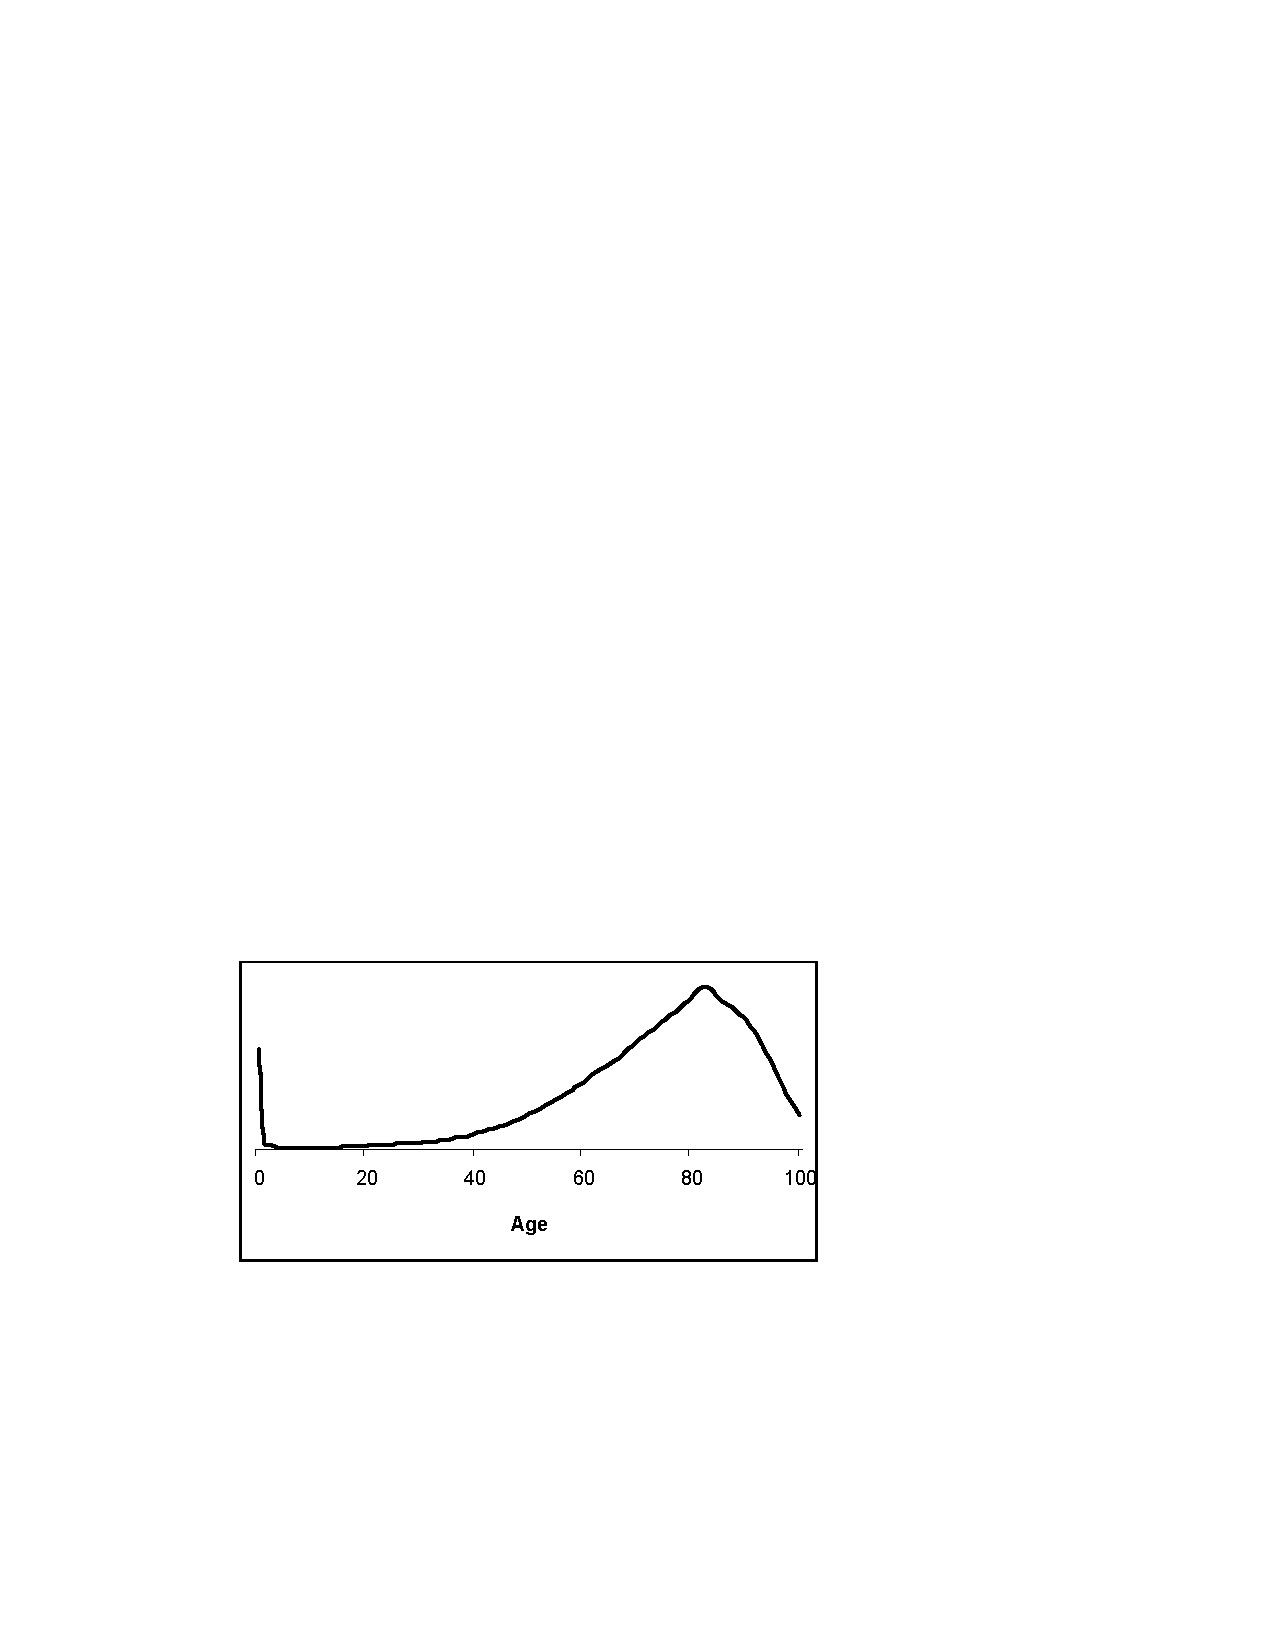
\includegraphics[width=8cm]{Graphs/Quiz2.pdf}
\end{center}
Which of the following functions of age does the graph most likely show?\footnote[4]{SOA MLC Sample Questions \# 106.}

\vspace{0.35cm}
\small
\begin{center}
\begin{tabular}{c c c c c}
(a) $\mu_x\;\;\;\;\;\;\;\;$ & 
$\;\;\;\;\;\;\;\;$(b) ${l_x\,\mu_x}\;\;\;\;\;\;\;\;$ &
$\;\;\;\;\;\;\;\;$(c) ${l_x\,p_x}\;\;\;\;\;\;\;\;$ & 
$\;\;\;\;\;\;\;\;$(d) ${l_x} \;\;\;\;\;\;\;\;$ &
$\;\;\;\;\;\;\;\;$(e) ${l_x^2}$ 
\end{tabular}
\end{center}

\end{enumerate}

\newpage

%==============================================================
%==============================================================


\thispagestyle{empty}
\setcounter{page}{1}
\begin{center}
{ \large \bf Life Contingencies I (AS4340), Quiz 3 (09/21/2011)}
\end{center}
\noindent
Circle the correct answer! Name: $\underline{\;\;\;\;\;\;\;\;\;\;\;\;\;\;\;\;\;\;\;\;\;\;\;\;\;\;\;\;\;\;\;\;\;\;\;\;\;\;\;\;\;\;\;\;\;\;\;\;\;\;\;\;\;}$
\begin{enumerate}
\item
You are given:
\begin{enumerate}
\item Deaths are uniformly distributed over each year of age.
\item $q_{x+3} = 0.101$.
\end{enumerate}
Calculate $_{0.5}q_{x+3.5}$.\footnote[1]{SOA Sample Questions \# 276 -- modified.}

\vspace{0.25cm}
\small
\begin{center}
\begin{tabular}{c c c c c}
(a) 0.046$\;\;\;\;\;\;\;\;$ & 
$\;\;\;\;\;\;\;\;$(b) 0.048$\;\;\;\;\;\;\;\;$ & 
$\;\;\;\;\;\;\;\;$(c) 0.051$\;\;\;\;\;\;\;\;$ &
$\;\;\;\;\;\;\;\;$(d) 0.053$\;\;\;\;\;\;\;\;$ &
$\;\;\;\;\;\;\;\;$(e) 0.056
\end{tabular}
\end{center}
\vspace{0.1cm}

\normalsize
\item For a 4-year college, you are given the following probabilities for dropout from all causes:

\begin{center}
\begin{tabular}{c c c c}
$q_0=0.15\;\;\;\;\;\;$ & 
$\;\;\;\;\;\;$$q_1=0.20\;\;\;\;\;\;$ & 
$\;\;\;\;\;\;$$q_2=0.10\;\;\;\;\;\;$ &
$\;\;\;\;\;\;$$q_3=0.01\;\;\;\;\;\;$ 
\end{tabular}
\vspace{0.1cm}
\end{center}

Dropouts are uniformly distributed over each year.

Compute the temporary 1.5-year complete expected college lifetime of a student entering the second year, $\stackrel{\circ}{e}_{1:\overline{1.5}|}$.\footnote[2]{SOA Sample Questions \# 120 -- modified numbers.} 

\vspace{0.25cm}
\small
\begin{center}
\begin{tabular}{c c c c c}
(a) 1.1$\;\;\;\;\;\;\;\;$ & 
$\;\;\;\;\;\;\;\;$(b) 1.2$\;\;\;\;\;\;\;\;$ & 
$\;\;\;\;\;\;\;\;$(c) 1.3$\;\;\;\;\;\;\;\;$ &
$\;\;\;\;\;\;\;\;$(d) 1.4$\;\;\;\;\;\;\;\;$ &
$\;\;\;\;\;\;\;\;$(e) 1.5
\end{tabular}
\end{center}
\vspace{0.1cm}

\normalsize
\item The actuarial department for the SharpPoint Corporation models the lifetime of pencil sharpeners from purchase using the survival function
$$
s(x) = \left(1 - \frac{x}{\omega}\right)^{\alpha}, \text{ for }\alpha >0 \text{ and } 0 \leq x \leq \omega.
$$
A senior actuary examining mortality tables for pencil sharpeners has determined that the original value of $\alpha$ must change. You are given:
\begin{enumerate}
\item The new complete expectation of life at purchase is half what it was previously.
\item The new force of mortality for pencil sharpeners is 3 times the previous force of mortality for all durations.
\item $\omega$ remains the same.
\end{enumerate}
Calculate the original value of $\alpha$.\footnote[3]{SOA Exam M Fall 2005 \# 13 -- modified numbers.}

\vspace{0.25cm}
\small
\begin{center}
\begin{tabular}{c c c c c}
(a) $1\;\;\;\;\;\;\;\;\;\;$ & 
$\;\;\;\;\;\;\;\;\;\;$(b) $2\;\;\;\;\;\;\;\;\;\;$ &
$\;\;\;\;\;\;\;\;\;\;$(c) $3\;\;\;\;\;\;\;\;\;\;$ & 
$\;\;\;\;\;\;\;\;\;\;$(d) $4 \;\;\;\;\;\;\;\;\;\;$ &
$\;\;\;\;\;\;\;\;\;\;$(e) $5$ 
\end{tabular}
\end{center}
\vspace{0.1cm}

\newpage
\normalsize

\item You are given:
\begin{enumerate}
\item $T$ is the future lifetime random variable
\item $\mu_t=\mu\;,\;\;t \geq 0$
\item $Var[T] = 81$
\item $X=\min\{T,10\}$
\end{enumerate}
Calculate $E[X]$.\footnote[4]{SOA MLC Sample Questions \# 189 -- modified numbers.}

\vspace{0.35cm}
\small
\begin{center}
\begin{tabular}{c c c c c}
(a) $5.4\;\;\;\;\;\;\;\;$ & 
$\;\;\;\;\;\;\;\;$(b) $5.7\;\;\;\;\;\;\;\;$ &
$\;\;\;\;\;\;\;\;$(c) $6.0\;\;\;\;\;\;\;\;$ & 
$\;\;\;\;\;\;\;\;$(d) $6.3 \;\;\;\;\;\;\;\;$ &
$\;\;\;\;\;\;\;\;$(e) $6.6$ 
\end{tabular}
\end{center}

%\item You are given the following information on participants entering a special 2-year program for treatment of a disease:
%\begin{enumerate}
%\item Only 10\% survive to the end of the second year. 
%\item The force of mortality is constant within each year. 
%\item The force of mortality for year 2 is three times the force of mortality for year 1.
%\end{enumerate}
%Calculate the probability that a participant who survives to the end of month 3 dies by the end of month 21.\footnote[4]{SOA Sample Questions \# 219.}

%\vspace{0.35cm}
%\small
%\begin{center}
%\begin{tabular}{c c c c c}
%(a) $0.61\;\;\;\;\;\;\;\;$ & 
%$\;\;\;\;\;\;\;\;$(b) $0.66\;\;\;\;\;\;\;\;$ &
%$\;\;\;\;\;\;\;\;$(c) $0.71\;\;\;\;\;\;\;\;$ & 
%$\;\;\;\;\;\;\;\;$(d) $0.75 \;\;\;\;\;\;\;\;$ &
%$\;\;\;\;\;\;\;\;$(e) $0.82$ 
%\end{tabular}
%\end{center}
\end{enumerate}

%==============================================================
%==============================================================

\newpage

\thispagestyle{empty}
\setcounter{page}{1}
\begin{center}
{ \large \bf Life Contingencies I (AS4340), Quiz 4 (10/19/2011)}
\end{center}
\noindent
Circle the correct answer! Name: $\underline{\;\;\;\;\;\;\;\;\;\;\;\;\;\;\;\;\;\;\;\;\;\;\;\;\;\;\;\;\;\;\;\;\;\;\;\;\;\;\;\;\;\;\;\;\;\;\;\;\;\;\;\;\;}$
\begin{enumerate}
\item For a special 3-year term insurance on $(x)$ you are given: 
\begin{enumerate}
\item $Z$ is the present-value random variable for this insurance.
\item $q_{x+k} = 0.02(k+1),$ $k=0,1,2$.
\item The following benefits are payable at the end of the year of death:
\begin{center}
\begin{tabular}{l || c | c | c}
$k$ & 0 & 1 & 2\\
\hline
\hline
$b_{k+1}$ & 300,000 & 350,000 & 400,000 \\
\end{tabular}
\end{center}
\item $i=0.06$.
\end{enumerate}
Calculate $E[Z]$.\footnote[1]{SOA Sample Questions \# 109.}

\begin{center}
\small
\begin{tabular}{c c c c c}
(a) $36,800\;\;\;\;$ & 
$\;\;\;\;\;\;$(b) $39,100\;\;\;\;$ &
$\;\;\;\;\;\;$(c) $41,400\;\;\;\;$ & 
$\;\;\;\;\;\;$(d) $43,700\;\;\;\;$ &
$\;\;\;\;\;\;$(e) $46,000$
\end{tabular}
\end{center}

\normalsize


\item For a special whole life insurance on $(x)$, you are given:
\begin{enumerate}
\item $Z$ is the present value random variable for this insurance.
\item Death benefits are paid at the moment of death.
\item $\mu_{x+t} = 0.02,$ $t \geq 0$ and $\delta =0.08.$
\item $b_t = e^{0.03\,t},$ $t \geq 0$.
\end{enumerate}
Calculate $Var[Z]$.\footnote[2]{SOA Exam M Fall 2005 No.\ 1.} 

\begin{center}
\small
\begin{tabular}{c c c c c}
(a) $0.075\;\;\;\;\;\;$ & 
$\;\;\;\;\;\;\;\;$(b) $0.080\;\;\;\;\;\;$ &
$\;\;\;\;\;\;\;\;$(c) $0.085\;\;\;\;\;\;$ & 
$\;\;\;\;\;\;\;\;$(d) $0.090\;\;\;\;\;\;$ &
$\;\;\;\;\;\;\;\;$(e) $0.095$
\end{tabular}
\end{center}



\normalsize

\item[$\rightarrow$] \textbf{For problems 3.\ and 4.}\\
You are given the following information from a life table where $i=0.06$. Assume a uniform distribution of deaths over each year of age.

\begin{center}
\begin{tabular}{|| c  | c | c||}
\hline
Age $x$ &  $1,000\,\left({A_x}\right)$ & $1,000\,\left({^2A_x}\right)$ \\
\hline
60 & 369.13 & 177.41 \\
\hline
\end{tabular}
\end{center}
%\vspace{0.3cm}

\normalsize
\item Calculate the variance for a whole life insurance on $(60)$ paying a level benefit of $\$100$ at the \textbf{moment} of death.

\begin{center}
\small
\begin{tabular}{c c c c c}
(a) $411.5\;\;\;\;\;\;\;\;$ & 
$\;\;\;\;\;\;\;\;$(b) $432.6\;\;\;\;\;\;\;\;$ &
$\;\;\;\;\;\;\;\;$(c) $434.8\;\;\;\;\;\;\;\;$ & 
$\;\;\;\;\;\;\;\;$(d) $436.9\;\;\;\;\;\;\;\;$ &
$\;\;\;\;\;\;\;\;$(e) $439.0$
\end{tabular}
\normalsize
%\vspace{0.1cm}
\end{center}

\item Calculate the variance of a whole life insurance on $(60)$ paying one unit at the end of the \textbf{month} of death.

\begin{center}
\small
\begin{tabular}{c c c c c}
(a) $0.04115\;\;\;\;\;$ & 
$\;\;\;\;\;$(b) $0.04326\;\;\;\;\;$ &
$\;\;\;\;\;$(c) $0.04348\;\;\;\;\;$ & 
$\;\;\;\;\;$(d) $0.04369\;\;\;\;\;$ &
$\;\;\;\;\;$(e) $0.04390$
\end{tabular}
\normalsize
%\vspace{0.1cm}
\end{center}

\end{enumerate}
%============================




%==============================================================
%==============================================================

\newpage

\thispagestyle{empty}
\setcounter{page}{1}
\begin{center}
{ \large \bf Life Contingencies I (AS4340), Take-Home Quiz 5 (Due 10/31/2011)}
\end{center}
\noindent
Print, circle the correct answer, and hand in! Name: $\underline{\;\;\;\;\;\;\;\;\;\;\;\;\;\;\;\;\;\;\;\;\;\;\;\;\;\;\;\;\;\;\;\;\;\;\;\;\;\;\;\;\;\;\;\;\;\;\;\;\;\;\;\;\;}$
\begin{enumerate}
\item You are given the following extract from a select-and-ultimate mortality table:
\begin{center}
\begin{tabular}{c || c c c || c}
$x$ & $l_{[x]}$ & $l_{[x]+1}$ & $l_{x+2}$ & $x+2$\\
\hline
60 & 80,625 & 79,954 & 78,839 & 62\\
61 & 79,137 & 78,402 & 77,252 & 63\\
62 & 77,575 & 76,770 & 75,578 &  64\\ 
\end{tabular}
\end{center}
Assume that deaths are uniformly distributed between integral ages.\\
Calculate ${_{0.9}q_{[60]+0.6}}$.\footnote[1]{SOA M Sample Questions and Solutions  No.\ 136.}
\vspace{0.1cm}
\begin{center}
\small
\begin{tabular}{c c c c c}
(a) $0.0102\;\;\;\;\;$ & 
$\;\;\;\;\;\;\;$(b) $0.0103\;\;\;\;\;$ &
$\;\;\;\;\;\;\;$(c) $0.0104\;\;\;\;\;$ & 
$\;\;\;\;\;\;\;$(d) $0.0105\;\;\;\;\;$ &
$\;\;\;\;\;\;\;$(e) $0.0106$
\end{tabular}
\end{center}
\vspace{0.1cm}

\normalsize

\item For a select-and-ultimate mortality table with a 3-year select period:
\begin{enumerate}
\item
\footnotesize
\begin{tabular}{c || c c c c || c}
$x$ & $q_{[x]}$ & $q_{[x]+1}$ & $q_{[x]+2}$ & $q_{x+3}$ & $x+3$\\
\hline
60 & 0.09 & 0.11 & 0.13 & 0.15 & 63\\
61 & 0.10 & 0.12 & 0.14 & 0.16 & 64\\
62 & 0.11 & 0.13 & 0.15 & 0.17 & 65\\
63 & 0.12 & 0.14 & 0.16 & 0.18 & 66\\
64 & 0.13 & 0.15 & 0.17 & 0.19 & 67\\
\end{tabular}
\normalsize
\item White was a newly selected life on 01/01/2000.
\item White's age on 01/01/2001 is 61.
\item $P$ is the probability on 01/01/2001 that White will be alive on 01/01/2006.
\end{enumerate}
Calculate $P$.\footnote[2]{SOA M Sample Questions and Solutions  No.\ 66.}

\vspace{0.1cm}
\begin{center}
\small
\begin{tabular}{l c r}
$\text{(a)}\;0 \leq P < 0.43\;\;\;\;\;\;\;\;\;\;$ & 
$\;\;\;\;\;\;\;\;\;\;\text{(b)}\;0.43 \leq P < 0.45\;\;\;\;\;\;\;\;\;\;$ & 
$\;\;\;\;\;\;\;\;\;\;\text{(c)}\;0.45 \leq P < 0.47$ \\
&&\\
$\text{(d)}\;0.47 \leq P < 0.49\;\;\;\;\;\;\;\;\;\;$ &&
$\;\;\;\;\;\;\;\;\;\;\text{(e)}\;0.49 \leq P \leq 1.00$
\end{tabular}
\end{center}
\vspace{0.1cm}

\normalsize

\item For a continuously increasing whole life insurance on $(x)$, you are given:
\begin{enumerate}
\item The force of mortality is constant.
\item $\delta = 0.09$
\item ${^2\bar{A}_x} = 0.25$
\end{enumerate}
Calculate $\left(\bar{I}\bar{A}\right)_x$.\footnote[3]{SOA M Sample Questions and Solutions No.\ 56 (changed numbers).}

\vspace{0.1cm}
\begin{center}
\small
\begin{tabular}{c c c c c}
(a) $0.6\;\;\;\;\;\;\;\;$ & 
$\;\;\;\;\;\;\;\;\;\;$(b) $1.3\;\;\;\;\;\;\;\;$ &
$\;\;\;\;\;\;\;\;\;\;$(c) $2.0\;\;\;\;\;\;\;\;$ & 
$\;\;\;\;\;\;\;\;\;\;$(d) $2.7\;\;\;\;\;\;\;\;$ &
$\;\;\;\;\;\;\;\;\;\;$(e) $3.4$
\end{tabular}
\end{center}
\vspace{0.1cm}

\item For a continuous whole life annuity of 1 on $(x)$:
\begin{itemize}
\item $T_x$ is the future lifetime random variable for $(x)$.
\item The force of interest and force of mortality are constant and equal.
\item $\bar{a}_x = 15.00.$ 
\end{itemize}
Calculate the standard deviation of $\bar{a}_{\overline{T_x}|}$.\footnote[4]{SOA M Sample Questions and Solutions No.\ 67 (changed numbers).}

\vspace{0.1cm}
\begin{center}
\small
\begin{tabular}{c c c c c}
(a) $5.8\;\;\;\;\;\;\;\;$ & 
$\;\;\;\;\;\;\;\;\;\;$(b) $7.2\;\;\;\;\;\;\;\;$ &
$\;\;\;\;\;\;\;\;\;\;$(c) $8.7\;\;\;\;\;\;\;\;$ & 
$\;\;\;\;\;\;\;\;\;\;$(d) $9.6\;\;\;\;\;\;\;\;$ &
$\;\;\;\;\;\;\;\;\;\;$(e) $14.7$
\end{tabular}
\end{center}
\vspace{0.1cm}

\normalsize

\item For a group of lives aged $x$, you are given:
\begin{itemize}
\item Each member of the group has a constant force of mortality that is drawn from the uniform distribution on $[0.03\,,\,0.05]$.
\item $\delta = 0.02$.
\end{itemize}
For a member selected at random from this group, calculate the actuarial present value of a continuous lifetime annuity of 1 per year.\footnote[5]{SOA Exam M Fall 2005 No.\ 20 (changed numbers).}

\vspace{0.1cm}
\begin{center}
\small
\begin{tabular}{c c c c c}
(a) $8.9\;\;\;\;\;\;\;\;$ & 
$\;\;\;\;\;\;\;\;$(b) $16.8\;\;\;\;\;\;\;\;$ &
$\;\;\;\;\;\;\;\;$(c) $24.7\;\;\;\;\;\;\;\;$ & 
$\;\;\;\;\;\;\;\;$(d) $32.7\;\;\;\;\;\;\;\;$ &
$\;\;\;\;\;\;\;\;$(e) $40.6$
\end{tabular}
\normalsize
\end{center}
\vspace{0.1cm}

\item Company ABC sets the gross premium for a continuous life annuity of 1 per year on $(x)$ equal to the actuarial present value calculated using:
\begin{enumerate}
\item $\delta = 0.03.$
\item $\mu_{x+t} = 0.02,\;t\geq 0.$ 
\end{enumerate}
However, a revised mortality assumption reflects future mortality improvement and is given by
$$
\mu_{x+t} = \left\{\begin{array}{l l}
0.02 & \text{ for } t \leq 10,\\
0.01 & \text {for } t > 10.
\end{array}\right.
$$
Calculate the expected loss at issue for ABC (using the revised mortality assumption) as a percentage of the gross premium.\footnote[6]{SOA M Sample Questions and Solutions No.\ 174.}

\vspace{0.1cm}
\begin{center}
\small
\begin{tabular}{c c c c c}
(a) $2\%\;\;\;\;\;\;\;\;$ & 
$\;\;\;\;\;\;\;\;$(b) $8\%\;\;\;\;\;\;\;\;$ &
$\;\;\;\;\;\;\;\;$(c) $15\%\;\;\;\;\;\;\;\;$ & 
$\;\;\;\;\;\;\;\;$(d) $20\%\;\;\;\;\;\;\;\;$ &
$\;\;\;\;\;\;\;\;$(e) $23\%$
\end{tabular}
\normalsize
\end{center}
\vspace{0.1cm}
	

\end{enumerate}
%============================

%==============================================================
%==============================================================

\newpage

\thispagestyle{empty}
\setcounter{page}{1}
\begin{center}
{ \large \bf Life Contingencies I (AS4340), Quiz 6 (11/02/2011)}
\end{center}
\noindent
Circle the correct answer! Name: $\underline{\;\;\;\;\;\;\;\;\;\;\;\;\;\;\;\;\;\;\;\;\;\;\;\;\;\;\;\;\;\;\;\;\;\;\;\;\;\;\;\;\;\;\;\;\;\;\;\;\;\;\;\;\;}$
\begin{enumerate}
\item For a continuously increasing whole life insurance on $(x)$, you are given:
\begin{enumerate}
\item The force of mortality is constant.
\item $\delta = 0.06$
\item ${^2\bar{A}_x} = 0.25$
\end{enumerate}
Calculate $\left(\bar{I}\bar{A}\right)_x$.\footnote[1]{SOA M Sample Questions No.\ 56.}

\vspace{0.1cm}
\begin{center}
\small
\begin{tabular}{c c c c c}
(a) $2.889\;\;\;\;\;\;\;$ & 
$\;\;\;\;\;\;\;\;\;$(b) $3.125\;\;\;\;\;\;\;$ &
$\;\;\;\;\;\;\;\;\;$(c) $4.000\;\;\;\;\;\;\;$ & 
$\;\;\;\;\;\;\;\;\;$(d) $4.667\;\;\;\;\;\;\;$ &
$\;\;\;\;\;\;\;\;\;$(e) $5.500$
\end{tabular}
\end{center}
\vspace{0.1cm}

\normalsize



\item For a group of lives aged $x$, you are given:
\begin{itemize}
\item Each member of the group has a constant force of mortality that is drawn from the uniform distribution on $[0.01\,,\,0.02]$.
\item $\delta = 0.01$.
\end{itemize}
For a member selected at random from this group, calculate the actuarial present value of a continuous lifetime annuity of 1 per year.\footnote[2]{SOA M Sample Questions No.\ 192.}

\vspace{0.1cm}
\begin{center}
\small
\begin{tabular}{c c c c c}
(a) $40.0\;\;\;\;\;\;\;\;$ & 
$\;\;\;\;\;\;\;\;$(b) $40.5\;\;\;\;\;\;\;\;$ &
$\;\;\;\;\;\;\;\;$(c) $41.1\;\;\;\;\;\;\;\;$ & 
$\;\;\;\;\;\;\;\;$(d) $41.7\;\;\;\;\;\;\;\;$ &
$\;\;\;\;\;\;\;\;$(e) $42.3$
\end{tabular}
\normalsize
\end{center}
\vspace{0.1cm}

\item For a 20-year continuous deferred whole life annuity of 1 per year on $(50)$, you are given
\begin{itemize}
\item Mortality follows De Moivre's law with $\omega = 100$.
\item $\delta=5\%$.
\end{itemize}
Calculate the probability that the sum of the annuity payments actually made will exceed the actuarial present value at issue of the annuity.\footnote[3]{Similar to SOA M Sample Questions and Solutions No.\ 55.}

\vspace{0.1cm}
\begin{center}
\small
\begin{tabular}{c c c c c}
(a) $40\%\;\;\;\;\;\;\;\;$ & 
$\;\;\;\;\;\;\;\;$(b) $43\%\;\;\;\;\;\;\;\;$ &
$\;\;\;\;\;\;\;\;$(c) $46\%\;\;\;\;\;\;\;\;$ & 
$\;\;\;\;\;\;\;\;$(d) $49\%\;\;\;\;\;\;\;\;$ &
$\;\;\;\;\;\;\;\;$(e) $52\%$
\end{tabular}
\normalsize
\end{center}
\end{enumerate}

\newpage
%==============================================================
%==============================================================

\thispagestyle{empty}
\setcounter{page}{1}
\begin{center}
{ \large \bf Life Contingencies I (AS4340), (Take-Home) Quiz 7 (11/09/2011)}
\end{center}
\noindent
Please print out the quiz, circle the correct answer, and hand it on Monday, 11/14/2011.\\
Name: $\underline{\;\;\;\;\;\;\;\;\;\;\;\;\;\;\;\;\;\;\;\;\;\;\;\;\;\;\;\;\;\;\;\;\;\;\;\;\;\;\;\;\;\;\;\;\;\;\;\;\;\;\;\;\;}$
\begin{enumerate}

\item For a 20-year deferred whole life annuity-due of 1 per year on $(50)$, you are given
\begin{itemize}
\item Mortality follows De Moivre's law with $\omega = 100$.
\item $i=0$.
\end{itemize}
Calculate the probability that the sum of the annuity payments actually made will exceed the actuarial present value at issue of the annuity.\footnote[1]{SOA Exam M Sample Questions \# 55 (changed numbers).}

\begin{center}
\small
\begin{tabular}{c c c c c}
(a) $0.38\;\;\;\;\;\;\;$ & 
$\;\;\;\;\;\;\;$(b) $0.40\;\;\;\;\;\;\;\;$ &
$\;\;\;\;\;\;\;$(c) $0.42\;\;\;\;\;\;\;$ & 
$\;\;\;\;\;\;\;$(d) $0.44\;\;\;\;\;\;\;$ &
$\;\;\;\;\;\;\;$(e) $0.46$
\end{tabular}
\end{center}
\normalsize

\item For a three year temporary life annuity-due of 100 on $(75)$, you are given
\begin{itemize}
\item $\int_0^x\mu(t)\,dt = 0.01\,x^{1.2},\,x>0$.
\item $i=8\%$.
\end{itemize}
Calculate the actuarial present value of this annuity.\footnote[2]{SOA Exam Spring 2007 \# 24 (changed numbers).}

\begin{center}
\small
\begin{tabular}{c c c c c}
(a) $265\;\;\;\;\;\;\;$ & 
$\;\;\;\;\;\;\;$(b) $267\;\;\;\;\;\;\;$ &
$\;\;\;\;\;\;\;$(c) $269\;\;\;\;\;\;\;$ & 
$\;\;\;\;\;\;\;$(d) $271\;\;\;\;\;\;\;$ &
$\;\;\;\;\;\;\;$(e) $273$
\end{tabular}
\end{center}
\normalsize

\item  For a pension plan portfolio, you are given
\begin{itemize}
\item 80 individuals with mutually independent future lifetimes are each to receive a whole life annuity-due.
\item $i=6\%$.
\item $\;$

\begin{center}
\small
\begin{tabular}{| c | c | c | c | c | c|}
\hline
Age & Number of annuitants & Annual Payment & $\ddot{a}_x$ & $A_x$ & ${^2A_x}$ \\
\hline
65 & 50 & 4 & 9.8969 & 0.43980 & 0.23603 \\
75 & 30 & 2 & 7.2170 & 0.59149 & 0.38681 \\ 
\hline
\end{tabular}
\end{center}
\end{itemize}
\normalsize
Using the normal approximation, calculate the 95th percentile of the distribution of the present random variable of this portfolio.\footnote[3]{SOA Exam Fall 2006 \# 4 (changed numbers).}

\begin{center}
\small\begin{tabular}{c c c c c}
(a) $1296\;\;\;\;\;\;\;$ & 
$\;\;\;\;\;\;\;$(b) $1944\;\;\;\;\;\;\;$ &
$\;\;\;\;\;\;\;$(c) $2593\;\;\;\;\;\;\;$ & 
$\;\;\;\;\;\;\;$(d) $4537\;\;\;\;\;\;\;$ &
$\;\;\;\;\;\;\;$(e) $5186$
\end{tabular}
\end{center}
\normalsize

\item For an annuity payable semiannually, you are given:
\begin{itemize}
\item Deaths are uniformly distributed over each year of age.
\item $q_{69}=0.03$
\item $i=0.06$
\item $1000\, \bar{A}_{70}=530$
\end{itemize} 
Calculate $\ddot{a}_{69}^{(2)}$.\footnote[4]{SOA Exam M Sample Questions \# 7.}

\begin{center}
\small
\begin{tabular}{c c c c c}
(a) $8.35\;\;\;\;\;\;\;$ & 
$\;\;\;\;\;\;\;$(b) $8.47\;\;\;\;\;\;\;$ &
$\;\;\;\;\;\;\;$(c) $8.59\;\;\;\;\;\;\;$ & 
$\;\;\;\;\;\;\;$(d) $8.72\;\;\;\;\;\;\;$ &
$\;\;\;\;\;\;\;$(e) $8.85$
\end{tabular}
\end{center}


\item Your company is competing to sell a life annuity-due with an actuarial present value of
500,000 to a 50-year old individual.

Based on your company's experience, typical 50-year old annuitants have a complete life expectancy of 25 years. However, this individual is not as healthy as your company's
typical annuitant, and your medical experts estimate that his complete life expectancy is
only 15 years.

You decide to price the benefit using the issue age that produces a complete life expectancy of 15 years. You also assume:
\begin{itemize}
\item For typical annuitants of all ages, mortality follows De Moivre's Law with the
same limiting age, $\omega$.
\item $i = 0.06$
\end{itemize}
Calculate the annual benefit that your company can offer to this individual.\footnote[5]{SOA Exam M Sample Questions \# 45.}

\begin{center}
\small
\begin{tabular}{c c c c c}
(a) $38,000\;\;\;\;\;$ & 
$\;\;\;\;\;$(b) $41,000\;\;\;\;\;$ &
$\;\;\;\;\;$(c) $46,000\;\;\;\;\;$ & 
$\;\;\;\;\;$(d) $49,000\;\;\;\;\;$ &
$\;\;\;\;\;$(e) $52,000$
\end{tabular}
\end{center}
\normalsize

\item At interest rate $i$:
\begin{itemize}
\item $\ddot{a}_x = 5.6$
\item The actuarial present value of a 2-year certain and life annuity-due of $1$ on $(x)$ is 
$\ddot{a}_{\overline{x:\overline{2}|}}=5.6459$.
\item $e_x = 8.83$
\item $e_{x+1}=8.29$
\end{itemize} 
Calculate $i$.\footnote[6]{SOA Exam M Sample Questions \# 88.}

\begin{center}
\small
\begin{tabular}{c c c c c}
(a) $0.077\;\;\;\;\;\;\;$ & 
$\;\;\;\;\;\;\;$(b) $0.079\;\;\;\;\;\;\;$ &
$\;\;\;\;\;\;\;$(c) $0.081\;\;\;\;\;\;\;$ & 
$\;\;\;\;\;\;\;$(d) $0.083\;\;\;\;\;\;\;$ &
$\;\;\;\;\;\;\;$(e) $0.084$
\end{tabular}
\end{center}
\normalsize
\end{enumerate}

%=============================================

\newpage

\thispagestyle{empty}
\setcounter{page}{1}
\begin{center}
{ \large \bf Life Contingencies I (AS4340), Quiz 8 (11/15/2011)}
\end{center}
\noindent
Circle the correct answer! Name: $\underline{\;\;\;\;\;\;\;\;\;\;\;\;\;\;\;\;\;\;\;\;\;\;\;\;\;\;\;\;\;\;\;\;\;\;\;\;\;\;\;\;\;\;\;\;\;\;\;\;\;\;\;\;\;}$
\begin{enumerate}
\item  For a pension plan portfolio, you are given
\begin{itemize}
\item 80 individuals with mutually independent future lifetimes are each to receive a whole life annuity-due.
\item $i=6\%$.
\item The $95^{\text{th}}$ percentile of the standard normal distribution is $z_{95\%}= 1.6448$.
\item $\;$

\begin{center}
\small
\begin{tabular}{| c | c | c | c | c | c|}
\hline
Age & Number of annuitants & Annual Payment & $\ddot{a}_x$ & $A_x$ & ${^2A_x}$ \\
\hline
65 & 50 & 2 & 9.8969 & 0.43980 & 0.23603 \\
75 & 30 & 4 & 7.2170 & 0.59149 & 0.38681 \\ 
\hline
\end{tabular}
\end{center}
\end{itemize}
\normalsize
Using the normal approximation, calculate the 95th percentile of the distribution of the present random variable of this portfolio.\footnote[1]{SOA Exam Fall 2006 \# 4 (changed numbers).}

\begin{center}
\small\begin{tabular}{c c c c c}
(a) $1296\;\;\;\;\;\;\;$ & 
$\;\;\;\;\;\;\;$(b) $2005\;\;\;\;\;\;\;$ &
$\;\;\;\;\;\;\;$(c) $2593\;\;\;\;\;\;\;$ & 
$\;\;\;\;\;\;\;$(d) $3005\;\;\;\;\;\;\;$ &
$\;\;\;\;\;\;\;$(e) $3568$
\end{tabular}
\end{center}
\normalsize

\item For a 20-year deferred whole life annuity-due of 1 per year on $(45)$, you are given
\begin{itemize}
\item Mortality follows De Moivre's law with $\omega = 105$.
\item $i=0$.
\end{itemize}
Calculate the probability that the sum of the annuity payments actually made will exceed the actuarial present value at issue of the annuity.\footnote[2]{SOA Exam M Sample Questions \# 55.}

\begin{center}
\small
\begin{tabular}{c c c c c}
(a) $0.425\;\;\;\;\;\;\;$ & 
$\;\;\;\;\;\;\;$(b) $0.450\;\;\;\;\;\;\;\;$ &
$\;\;\;\;\;\;\;$(c) $0.475\;\;\;\;\;\;\;$ & 
$\;\;\;\;\;\;\;$(d) $0.500\;\;\;\;\;\;\;$ &
$\;\;\;\;\;\;\;$(e) $0.525$
\end{tabular}
\end{center}
\normalsize


\item On January 1, 2002, Pat, age 40, purchases a 5-payment, 10-year term insurance of 100,000:
\begin{enumerate}
\item Death benefits are payable at the moment of death.
\item Contract premiums of 4000 are payable annually at the beginning of each year for 5 years.
\item $i=0.05$.
\item $L$ is the loss random variable at time of issue.
\end{enumerate}
Calculate the value of $L$ if Pat dies on June 30, 2004.\footnote[3]{SOA Sample Questions No.\ 99.}

\small
\begin{center}
\begin{tabular}{c c c c c}
(a) 77,100$\;\;\;\;\;\;\;$ & 
$\;\;\;\;\;\;\;$(b) 80,700$\;\;\;\;\;\;\;$ & 
$\;\;\;\;\;\;\;$(c) 82,700$\;\;\;\;\;\;\;$ &
$\;\;\;\;\;\;\;$(d) 85,900$\;\;\;\;\;\;\;$ &
$\;\;\;\;\;\;\;$(e) 88,000
\end{tabular}
\end{center}
\normalsize

\item A fund is established to pay annuities to 100 independent lives aged $x$. Each annuitant will receive 10,000 per year continuously until death. You are given:
\begin{enumerate}
\item $\delta = 0.06$.
\item $\bar{A}_x = 0.40$.
\item ${^2\bar{A}_x} = 0.25$.
\item The $90^{\text{th}}$ percentile of the standard normal distribution is $z_{90\%}= 1.282$.
\end{enumerate}
Calculate the amount (in millions) needed in the fund so that the probability, using the normal approximation, is $0.90$ that the fund will be sufficient to provide the payments.\footnote[4]{SOA Sample Questions No.\ 146.} 

\small
\begin{center}
\begin{tabular}{c c c c c}
(a) 9.74$\;\;\;\;\;\;\;$ & 
$\;\;\;\;\;\;\;$(b) 9.96$\;\;\;\;\;\;\;$ & 
$\;\;\;\;\;\;\;$(c) 10.30$\;\;\;\;\;\;\;$ &
$\;\;\;\;\;\;\;$(d) 10.64$\;\;\;\;\;\;\;$ &
$\;\;\;\;\;\;\;$(e) 11.10
\end{tabular}
\end{center}

\end{enumerate}

%============================
%==============================================================
\newpage
\thispagestyle{empty}
\setcounter{page}{1}
\begin{center}
{ \large \bf Life Contingencies I (AS4340), (Take-Home) Quiz 9 (11/28/2011)}
\end{center}
\noindent
Please print out the quiz, circle the correct answer, and hand it on Wednesday, 11/30/2011.\\
Name: $\underline{\;\;\;\;\;\;\;\;\;\;\;\;\;\;\;\;\;\;\;\;\;\;\;\;\;\;\;\;\;\;\;\;\;\;\;\;\;\;\;\;\;\;\;\;\;\;\;\;\;\;\;\;\;}$
\begin{enumerate}

\item For a fully continuous whole life insurance of 1 on $(x)$, you are given: 
\begin{enumerate}
\item  The forces of mortality and interest are constant.
\item $^2\bar{A}_x= 0.20$.
\item The benefit premium is 0.03.
\item $L$ is the loss-at-issue random variable based on the benefit premium. 
\end{enumerate}
Calculate $Var(L)$.%\footnote[1]{SOA Sample Questions No.\ 14.} 


\begin{center}
\small
\begin{tabular}{c c c c c}
(a) $0.20\;\;\;\;\;\;\;$ & 
$\;\;\;\;\;\;\;$(b) $0.21\;\;\;\;\;\;\;$ &
$\;\;\;\;\;\;\;$(c) $0.22\;\;\;\;\;\;\;$ & 
$\;\;\;\;\;\;\;$(d) $0.23\;\;\;\;\;\;\;$ &
$\;\;\;\;\;\;\;$(e) $0.24$
\end{tabular}
\end{center}
\normalsize

\item For a block of fully discrete whole life insurances of 1 on independent lives age $x$, you are given:
\begin{enumerate}
\item $i = 0.06$
\item $A_x = 0.24905$
\item $^2A_x = 0.09476$
\item $\pi = 0.025$, where $\pi$ is the premium for each policy. 
\end{enumerate}
Using the normal approximation, calculate the minimum number of policies the insurer must issue so that the probability of a positive total loss on the policies issued is less than or equal to 0.05.%\footnote[2]{SOA Sample Questions No.\ 24.} 

\small
\begin{center}
\begin{tabular}{c c c c c}
(a) 25$\;\;\;\;\;\;\;$ & 
$\;\;\;\;\;\;\;$(b) 27 $\;\;\;\;\;\;\;$ &
$\;\;\;\;\;\;\;$(c) 29$\;\;\;\;\;\;\;$ & 
$\;\;\;\;\;\;\;$(d) 31 $ \;\;\;\;\;\;\;$ &
$\;\;\;\;\;\;\;$(e) 33 $\;\;\;\;\;\;\;$ 
\end{tabular}
\end{center}
\normalsize

\item For a fully discrete whole life insurance of 100,000 on each of 10,000 lives age 60, you are given:
\begin{enumerate}
\item The future lifetimes are independent. Mortality follows the Illustrative Life Table.
\item $i = 0.06$. 
\item $\pi$ is the premium for each insurance of 100,000.
\end{enumerate}
Using the normal approximation, calculate $\pi$, such that the probability of a positive total loss
is 1\%.%\footnote[3]{SOA Sample Questions No.\ 60.} 

\small
\begin{center}
\begin{tabular}{c c c c c}
(a) 3340$\;\;\;\;\;\;\;$ & 
$\;\;\;\;\;\;\;$(b) 3360  $\;\;\;\;\;\;\;$ &
$\;\;\;\;\;\;\;$(c) 3380$\;\;\;\;\;\;\;$ & 
$\;\;\;\;\;\;\;$(d) 3390 $ \;\;\;\;\;\;\;$ &
$\;\;\;\;\;\;\;$(e) 3400$\;\;\;\;\;\;\;$ 
\end{tabular}
\end{center}
\normalsize
\newpage
\item For a fully continuous whole life insurance of 1 on $(x)$:
\begin{enumerate}
\item $\pi$ is the benefit premium. 
\item $L$ is the loss-at-issue random variable with the premium equal to $\pi$ . 
\item $L^*$ is the loss-at-issue random variable with the premium equal to 1.25 $\pi$ .
\item $\bar{a}_x = 5.0$ 
\item $\delta = 0.08$.
\item $Var(L) = 0.5625$.
\end{enumerate}
Calculate the sum of the expected value and the standard deviation of $L^*$.%\footnote[4]{SOA Sample Questions No.\ 142.} 

\small
\begin{center}
\begin{tabular}{c c c c c}
(a) 0.59$\;\;\;\;\;\;\;$ & 
$\;\;\;\;\;\;\;$(b) 0.71  $\;\;\;\;\;\;\;$ &
$\;\;\;\;\;\;\;$(c) 0.86$\;\;\;\;\;\;\;$ & 
$\;\;\;\;\;\;\;$(d) 0.89 $ \;\;\;\;\;\;\;$ &
$\;\;\;\;\;\;\;$(e) 1.01$\;\;\;\;\;\;\;$ 
\end{tabular}
\end{center}
\normalsize

\item For a special fully continuous whole life insurance on $(x)$:
\begin{enumerate}
\item The level premium is determined using the equivalence principle. 
\item Death benefits are given by $b_t = (1+i)^t$ where $i$ is the interest rate.
\item  $L$ is the loss random variable at $t=0$ for the insurance. 
\item $T$ is the future lifetime random variable of $(x)$.
\end{enumerate}
Which of the following expressions is equal to L ?%\footnote[5]{SOA Sample Questions No.\ 119.} 

\small
\begin{center}
\begin{tabular}{l c l}
(a) $\frac{(v^T - \bar{A}_x)}{(1-\bar{A}_x)}$ $\;\;\;\;\;\;\;$ & 
$\;\;\;\;\;\;\;$(b) ${(v^T - \bar{A}_x)}{(1+\bar{A}_x)}$  $\;\;\;\;\;\;\;$ &
$\;\;\;\;\;\;\;$(c) $\frac{(v^T - \bar{A}_x)}{(1+\bar{A}_x)}$ \\
(d) ${(v^T - \bar{A}_x)}{(1-\bar{A}_x)}$ $\;\;\;\;\;\;\;$ & &
$\;\;\;\;\;\;\;$(e) $\frac{(v^T + \bar{A}_x)}{(1+\bar{A}_x)}$  
\end{tabular}
\end{center}
\normalsize

\item  For a fully discrete whole life insurance of 10,000 on (20):
\begin{enumerate}
\item $\pi$ denotes the annual premium and $L(\pi)$ denotes the loss-at-issue random variable for this insurance. 
\item Mortality follows the illustrative life table.
\item $i=0.06$.
\end{enumerate}
Calculate the lowest premium, $\pi'$, such that the probability is less than 20\% that the loss $L(\pi')$ is positive.%\footnote[6]{SOA Sample Questions No.\ 139 (changed numbers).} 


\small
\begin{center}
\begin{tabular}{c c c c c}
(a) 37.2$\;\;\;\;\;\;\;$ & 
$\;\;\;\;\;\;\;$(b) 39.2 $\;\;\;\;\;\;\;$ &
$\;\;\;\;\;\;\;$(c) 42.2$\;\;\;\;\;\;\;$ & 
$\;\;\;\;\;\;\;$(d) 44.2 $ \;\;\;\;\;\;\;$ &
$\;\;\;\;\;\;\;$(e) 47.2 $\;\;\;\;\;\;\;$ 
\end{tabular}
\end{center}

\end{enumerate}



%=============================================
\appendix
\thispagestyle{empty}
\chapter[Practice Questions]{}
\thispagestyle{empty}
\vspace{3cm}
\begin{center}
{\Huge \bf Practice Questions}
\end{center}

\newpage


\newpage

\setcounter{page}{1}
\normalsize
\begin{center}
{ \Huge \bf Practice Question}
\end{center}
\normalsize
\begin{enumerate}

\item Assume $\mu_{50}(t)=0.04$ and $\delta=0.06$. Mr.\ 50 buys a whole life insurance with a benefit of \$10,000 payable at the moment of death against level, continuous premium payments.
\begin{enumerate}
\item Calculate the annual benefit premium determined by the Equivalence Principle.
\item Calculate the standard deviation of the corresponding loss random variable $L$.
\item Assume now that this policy is sold to 1,000 different $(60)$-year olds with the same distribution of future lifetime. Calculate the probability that the insurer's loss at issue is greater than its annual premium income.
\item Assume now that this policy is sold to 1,000 different $(60)$-year olds with the same distribution of future lifetime. Calculate the portfolio percentile premium with $\gamma=5\%$, i.e.\ calculate the smallest premium such that the probability of a positive loss is smaller or equal to $5\%$.
\end{enumerate}
\item Use the illustrative life table $(i=6\%)$ to
\begin{enumerate}
\item Calculate $P_{60}$ as well as the variance of the corresponding loss random variable.
\item Calculate $\bar{P}(\bar{A}_{60:\overline{5}|})$.
\item Calculate $\bar{P}(\bar{A}_{60})$.
\item Calculate $_5\bar{P}(\bar{A}_{60})$. Is it greater or smaller than the values from (b) and (c). Explain!
\end{enumerate}
\item Under a uniform distribution of deaths over each year of age, use the illustrative life table ($i=6\%$) to calulate $A_{66}^{(12)}$ and $^2A_{66}^{(12)}$.
\item Assume mortality follows De Moivre's law with $\omega = 105$ and $\delta = 0.05$. Mr.\ (45) buys a continuous whole life annuity paying \$100 each year. Calculate:
\begin{enumerate}
\item The actuarial present value for the annuity contract.
\item The variance of the corresponding present value random variable.
\item The probability that the discounted payoff is less than the present value.
\end{enumerate}
\item Assume mortality follows De Moivre's mortality law with $\omega=100$ and $\delta=0.05$.
\begin{enumerate}
\item Calculate $\left(\bar{I}\bar{A}\right)_{40}$.
\item Without any calculation, make an inference of whether $\left(I\bar{A}\right)_{40}$ is greater or smaller than the value from (a). Please explain.
\end{enumerate}
\item  For Mr.\ (40), use the illustrative life table ($i=6\%$) to calculate:
\begin{enumerate}
\item The actuarial present value of a 10-year deferred life annuity-due of \$1 per year.
\item The actuarial present value of a 10-year temporary life annuity-due of \$1 per year.
\item The variance of the present value random variable for a whole-life annuity-due of \$1 per year.
\end{enumerate} 
\item Use the illustrative life table ($i=6\%$) to determine the probability that a $60.5$-year old will die in the next year assuming
\begin{enumerate}
\item a uniform distribution of deaths over each year of age.
\item a constant force of mortality over each year of age.
\end{enumerate}
\item Use the illustrative life table to claculate the probability that Mr.\ (50) will die between age $51\frac{1}{2}$ and $52\frac{1}{2}$, i.e.\ $_{{1.5}|1}q_{50}$, under
\begin{enumerate}
\item The assumption that deaths are uniformly distributed within each year of age.
\item The assumption of a constant force of mortality within each year of age.
\end{enumerate}
\item For Mr.\ (50), you are given that $\mu_{50}(t) = 0.02$. Calculate:
\begin{enumerate}
\item The probability that he dies before the age of 70.
\item His complete expected future lifetime.
\item The median of his future lifetime.
\end{enumerate}
\end{enumerate}


%============================================================================================


\normalsize
\newpage

\chapter[Exam]{}
\thispagestyle{empty}
\vspace{3cm}
\begin{center}
{\Huge \bf Exams}
\end{center}

\newpage

\thispagestyle{empty}
\setcounter{page}{1}


\thispagestyle{empty}


\includegraphics[height=2cm]{Graphs/wisc.png} 


\noindent \rule{\textwidth}{1.5pt}
%\begin{minipage}[b]{0.6\textwidth}
    \begin{flushright}
    \textbf{\large Life Contingencies I -- AS 4340}\\  	
       {\large Fall 2011}\\
   %     {\footnotesize (CRN 86561)}\\ 
    %\textbf{\large Syllabus}\\
    \end{flushright}
%\end{minipage}
\vspace{-1cm}

{\huge \textbf{Midterm Examination}}

%\vspace{2cm}
%{\large
%\begin{center}
%\begin{tabular}{|| l l ||}
%\hline
%\hline
%& \\
%\textbf{Name:} & \underline{$\;\;\;\;\;\;\;\;\;\;\;\;\;\;\;\;\;\;\;\;\;\;\;\;\;\;\;\;\;\;\;\;\;\;\;\;\;\;\;\;\;\;\;$} \\
%Examination time: & 75 minutes \\
%Total attainable points: & 53 (50 points are 100\%) \\
% & \\
%\hline
%\hline
%\end{tabular}\\
%\end{center}
%$\;\;\;\;\;\;\;\;\;\;\;\;\;\;\;\;\;$
%}

\vspace{0.5cm}

%{\large
%\begin{center}
%\begin{tabular}{|| l | c ||}
%\hline
%\hline
%Problem & $\;\;\;\;\;\;$ Points $\;\;\;\;\;\;$ \\
%\hline
%\hline
%1 & \\
%\hline
%2 & \\
%\hline
%3 & \\
%\hline
%4 & \\
%\hline
%5 (Bonus) & \\
%\hline
%\hline
%Total & \\
%\hline
%\hline
%\end{tabular}
%\end{center}
%}
%\vspace{0.5cm}

%\noindent \textbf{Notes:}
%\begin{itemize}
%\item Show all your work! 
%\item Circle your final answers!
%\end{itemize}

%\newpage

\begin{enumerate}

\item {\tt [3 + 4 + 4 + 2 pt]} Assume mortality follows the illustrative life table.
\begin{enumerate}
\item Determine $_{10|5}q_{30}$.
\item \label{EXAM11b} Determine ${_{7.5}p_{35.5}}$ under the assumption of a uniform distribution of deaths over each year of age.
\item \label{EXAM11c} Determine ${_{7.5}p_{35.5}}$ under the assumption of a constant force of mortality over each year of age.
\item Which of the two values in (\ref{EXAM11b}) and (\ref{EXAM11c}) is greater. Provide an explanation for your answer!
\end{enumerate}
 
%\newpage
%$\;$
%\newpage

\item {\tt [8 + 6 + 2 pt]} Assume mortality follows De Moivre's Law with $\omega = 100$ and that $\delta = 5\%$.
\begin{enumerate}
\item Determine the expected value and the variance of the present value random variable $Z$ of a 20-year endowment insurance paying \$1 at the moment of death or in case of survival on a life aged $(50)$.
\item Suppose now $N=100$ independent individuals aged $(50)$ buy 20-year endowment contracts with a payoff of \$1,000 each payable at the moment of death or in case of survival. Find an approximate value $\chi$ such that in 95\% of all cases, the discounted payoff for the insurance company will be smaller than ${\chi}$.
\item If the insurance company increases the number of insureds $N$, will $\frac{\chi}{N}$ increase or decrease? Provide an explanation for your answer.
\end{enumerate}

%\newpage
%$\;$
%\newpage

\item {\tt [4 + 7 + 2 pt]}  Let $\mu_{55+t} = 0.05$, $t\geq 0,$ and $\delta = 5\%$. 
\begin{enumerate}
\item \label{EXAM13a} Calculate $\bar{A}_{55}$ and $^2\bar{A}_{55}$.
\item \label{EXAM13b} Calculate $A_{55}$ and $^2{A}_{55}$.
\item Which of the expected values calculated in (\ref{EXAM13a}) and (\ref{EXAM13b}) is greater. Provide an explanation for your answer.
\end{enumerate}

%\newpage

\item {\tt [3 + 6 pt]} Assume mortality follows the illustrative life table.
\begin{enumerate}
\item Calculate $l_{66}$.
\item You are given that $e_{66} = 14.35$. Calculate $e_{65}$.
\end{enumerate}
{\small \it Hint: You are given $q_x$ in the 3rd column of the life table.}

%\newpage

\item {\tt [2 + 1 pt]} \textbf{Bonus Problem:} 
What is the covariance between an $n$-year term life insurance and an $n$-year deferred insurance? Is it positive or negative?

\end{enumerate}

%==============================================================
%==============================================================

\newpage

\thispagestyle{empty}
\setcounter{page}{1}


\thispagestyle{empty}


\includegraphics[height=2cm]{Graphs/wisc.png} 

\noindent \rule{\textwidth}{1.5pt}
%\begin{minipage}[b]{0.6\textwidth}
    \begin{flushright}
    \textbf{\large Life Contingencies I -- AS 4340}\\  	
       {\large Fall 2011}\\
   %     {\footnotesize (CRN 86561)}\\ 
    %\textbf{\large Syllabus}\\
    \end{flushright}
%\end{minipage}
\vspace{-1cm}

{\huge \textbf{Final Examination}}

\vspace{2cm}
{\large
\begin{center}
\begin{tabular}{|| l l ||}
\hline
\hline
& \\
\textbf{Name:} & \underline{$\;\;\;\;\;\;\;\;\;\;\;\;\;\;\;\;\;\;\;\;\;\;\;\;\;\;\;\;\;\;\;\;\;\;\;\;\;\;\;\;\;\;\;$} \\
Examination time: & 115 minutes \\
Total attainable points: & 55 (50 points are 100\%) \\
 & \\
\hline
\hline
\end{tabular}\\
\end{center}
$\;\;\;\;\;\;\;\;\;\;\;\;\;\;\;\;\;$
}

\vspace{0.5cm}

{\large
\begin{center}
\begin{tabular}{|| l | c ||}
\hline
\hline
Problem & $\;\;\;\;\;\;$ Points $\;\;\;\;\;\;$ \\
\hline
\hline
1 & \\
\hline
2 & \\
\hline
3 & \\
\hline
4 & \\
\hline
5 & \\
\hline
6 & \\
\hline
7 (Bonus) & \\
\hline
\hline
Total & \\
\hline
\hline
\end{tabular}
\end{center}
}
\vspace{0.5cm}

\noindent \textbf{Notes:}
\begin{itemize}
\item Show all your work! 
\item Tables are attached on the last pages of this exam.
\item Circle your final answers!
\end{itemize}

\newpage

\begin{enumerate}

\item {\tt [3 + 3 + 6 + 2 pt]}  Assume mortality follows De Moivre's Law with $\omega = 100$ and that $\delta = 5\%$. Mr.\ 50 buys a whole life insurance with a benefit of \$10,000 payable at the moment of death against level, continuous premium payments.
\begin{enumerate}
\item Calculate the annual benefit premium, $\bar{P}^E$, determined by the Equivalence Principle.
\item Calculate the standard deviation of the corresponding loss random variable $L$.
\item Assume now that this policy is sold to $N=1,000$ different (independent) $(50)$-year olds with the same distribution of future lifetime. Calculate the portfolio percentile premium with $\gamma=5\%$, i.e.\ calculate the smallest premium $\bar{P}^P$  such that the probability of a positive loss is smaller or equal to $5\%$.
\item If the insurance company increases the number of insureds $N$, will $\left(\bar{P}^P - \bar{P}^E \right)$ increase or decrease? Provide an explanation for your answer.
\end{enumerate}


 
\newpage
$\;$
\newpage

\item {\tt [5 + 4 + 2 pt]} Use the illustrative life table $(i=6\%)$ to:
\begin{enumerate}
\item \label{EX2a} Calculate $\bar{P}\left(\bar{A}_{60}\right)$ as well as the variance of the corresponding loss random variable.
\item \label{EX2b} Calculate $\bar{P}(\bar{A}_{60:\overline{5}|})$.
\item Is the value in (\ref{EX2a}) greater or smaller than the value from (\ref{EX2b}). Provide an explanation.
\end{enumerate}

\newpage
$\;$
\newpage

\item {\tt [2 + 3 pt]} Assume mortality follows the illustrative life table with $i=6\%$.
\begin{enumerate}
\item Calculate $l_{66}$.
\item Calculate $\ddot{a}_{66}^{(12)}$.
\end{enumerate}
{\small \it Hint: You are given $q_x$ in the 3rd column of the life table.}

\newpage

\item  {\tt [4 + 2 pt]} Assume $\mu_{50+t}=0.04$ and $\delta=0.06$. 
\begin{enumerate}
\item \label{Fin4a} Calculate $\left(\bar{I}\bar{A}\right)_{\stackrel{1}{50}:\overline{20}|}$.
\item Without any calculation, make an inference of whether $\left(I\bar{A}\right)_{\stackrel{1}{50}:\overline{20}|}$ is greater or smaller than the value from (\ref{Fin4a}). Please explain.
\end{enumerate}

\newpage

\item {\tt [2 + 3 + 2 + 2 pt]} Assume mortality follows the illustrative life table.
\begin{enumerate}
\item Determine $_{10|5}q_{40}$.
\item \label{EXAM11b} Determine ${_{7.5}p_{45.5}}$ under the assumption of a uniform distribution of deaths over each year of age.
\item \label{EXAM11c} Determine ${_{7.5}p_{45.5}}$ under the assumption of a constant force of mortality over each year of age.
\item Which of the two values in (\ref{EXAM11b}) and (\ref{EXAM11c}) is greater. Provide an explanation for your answer!
\end{enumerate}

\newpage

\item {\tt [2 + 3 pt]} Assume mortality follows De Moivre's Law with $\omega = 100$ . Calculate:
\begin{enumerate}
\item The probability that Mr.\ 50 dies before the age of 70.
\item The complete expected future lifetime for Mr.\ 50.
\end{enumerate}


\newpage

\item {\tt [5 pt]} \textbf{Bonus Problem:} Let $\mu_{x+t} = \mu$ be constant and $\delta>0$. Let $L$ denote the loss random variable for a whole life insurance policy payable at the moment of death on an $(x)$-year old, where level, continuous premium payments amount to $\bar{P}$ every year.

Show that 
$$
Pr(L \leq x) = \left(\frac{\bar{P} + x\,\delta}{\bar{P} + \delta}\right)^{\frac{\mu}{\delta}},\;
-\frac{\bar{P}}{\delta} \leq x \leq 1.
$$ \end{enumerate}




\end{document}
